\documentclass[]{report}
\usepackage[utf8]{inputenc}
\usepackage{geometry}
\geometry{a4paper,left=2cm,right=3cm, top=2.5cm, bottom=2cm} 


\usepackage{amsmath}
\usepackage{siunitx}
\usepackage{graphicx}
\usepackage{caption}
\usepackage{subcaption}

\usepackage{pgfplots}
% and optionally (as of Pgfplots 1.3):
\pgfplotsset{compat=newest}
\pgfplotsset{plot coordinates/math parser=false}
\newlength\figureheight
\newlength\figurewidth 
\setlength\figureheight{5cm}
\setlength\figurewidth{\textwidth}


% Title Page
\title{Gruppennummer 16}
\author{Andreas Cremer\\Hanna Huber\\Lena Trautmann}



\begin{document}
\maketitle

%\begin{abstract}
%\end{abstract}

\begin{enumerate}
	\item Kovarianzmatrix
	\begin{enumerate}
		\item
		ourCov.m erwartet eine $d \times n$ Matrix und gibt die dazugehörige Kovarianzmatrix zurück.
		\item
		Hier werden die Kovarianzmatrizen für daten.mat berechnet. In $C_{11}$ steht die Varianz in der ersten Dimension. In $C_{22}$ steht die Varianz in der zweiten Dimension. In $C_{12}$ und $C_{21}$ steht die Kovarianz.\\
		data1 hat eine hohe Varianz in der ersten und eine geringe Varianz in der zweiten Dimension. Die Kovarianz ist gering, die Datenpunkte bilden ein schmales Band parallel zur x-Achse.\\
		data2 hat eine geringe Varianz in der ersten und eine hohe Varianz in der zweiten Dimension und ebenfalls eine geringe Kovarianz. Die Datenpunkte bilden ein schmales Band parallel zur y-Achse.\\
		data3 hat eine sehr hohe und eine deutlich niedrigere Varianz sowie eine hohe Kovarianz. Dies führt zu einem leicht ansteigenden Band.
		data4 hat hohe nahe beieinander liegende Varianzen und eine Kovarianz nahe beim Nullpunkt. Dies führt zu einer Punktwolke ohne erkennbare Ordnung.
	\end{enumerate}
	\item PCA
	\begin{enumerate}
		
		\item
		\item
		Der erste Eigenvektor gibt die Richtung der höchsten Varianz an. Weitere Eigenvektoren stehen jeweils orthogonal auf alle schon vorhanden Eigenvektoren und geben die Richtung der höchsten verbleibenden Varianz an. Im Plot sind die Eigenvektoren durch blaue Striche durch den Mittelwert gekennzeichnet.
		\item
		Die Eigenwerte zu den Eigenvektoren geben die Varianz in Richtung des jeweiligen Eigenvektors an. Im Plot sind sie durch die Länge der Eigenvektormarkierungen dargestellt. Sie ergeben aufaddiert die Gesamtvarianz.
		\item
		In die Berechnung von Varianz und Kovarianz fließt hier der Abstand der Datenpunkte vom Nullpunkt des verwendeten Koordinatensystems mit ein. Somit kann man keine sinnvollen Schlussfolgerungen mehr ziehen. Durch den Mittelwertsabzug wird die Kovarianzmatrix invariant gegen Translation. 
		
	\end{enumerate}
	\item Unterraum-Projektion
	\begin{enumerate}
		\item
	\end{enumerate}
	
	\item Untersuchungen in 3D
	\begin{enumerate}
		\item
		\setlength\figureheight{5cm}
		\begin{figure}[tbp!]
			\centering
			% This file was created by matlab2tikz.
% Minimal pgfplots version: 1.3
%
%The latest updates can be retrieved from
%  http://www.mathworks.com/matlabcentral/fileexchange/22022-matlab2tikz
%where you can also make suggestions and rate matlab2tikz.
%
\definecolor{mycolor1}{rgb}{0.00000,0.44700,0.74100}%
%
\begin{tikzpicture}

\begin{axis}[%
width=0.834982\figurewidth,
height=\figureheight,
at={(0\figurewidth,0\figureheight)},
scale only axis,
xmin=15.8346377737708,
xmax=72.1974302448346,
tick align=outside,
xmajorgrids,
ymin=-195.899798342177,
ymax=-145.273430024653,
ymajorgrids,
zmin=0.23419827595693,
zmax=26.9925672397016,
zmajorgrids,
view={57.3}{-20.4},
axis x line*=bottom,
axis y line*=left,
axis z line*=left,
legend style={at={(1.03,1)},anchor=north west,legend cell align=left,align=left,draw=white!15!black}
]
\addplot3 [color=blue,only marks,mark=*,mark options={solid}]
 table[row sep=crcr] {%
52.9875244603804	-158.235197385273	19.6939120642748\\
37.1859590107583	-174.525805964515	14.6555970215217\\
43.5306124773317	-162.100629256904	21.0813680546959\\
66.852003959705	-154.124406930327	15.7890980880996\\
42.8817537873011	-165.229351622428	17.2368227406429\\
46.6514106811411	-169.599368118236	10.8809201965504\\
41.6334150149265	-161.480715212225	19.0464150181916\\
40.3938116980538	-171.412715876583	13.7543844527967\\
36.990310706045	-168.615857894668	13.1317759546028\\
38.2230830754718	-158.014430457988	20.8489722304474\\
32.5659673186649	-180.344443755414	13.5076325298726\\
40.6894226855553	-164.699007800179	17.6960911968818\\
37.9404092682918	-165.006741437259	17.3822567531133\\
40.1915059712317	-168.405675992741	7.62340860541223\\
47.3684349940829	-167.196057087138	14.1911412475499\\
45.982036953502	-164.360271984919	16.1923955518165\\
39.6905036364315	-173.598466684762	13.0947938876336\\
54.4018700175855	-152.905155410094	23.9979037901877\\
38.6960321145113	-166.425044208539	17.5801794236905\\
47.9455895229326	-170.981777086213	15.7086966763573\\
30.8401234703536	-167.638677661519	15.715948469452\\
29.8277101066108	-184.136824220921	8.17461001953879\\
34.0109656612976	-172.956174998167	15.3223339154196\\
45.0056296161848	-166.114986907029	17.8090037636074\\
47.2141243224894	-158.697938485232	16.2442373658733\\
42.9280086822335	-167.621019318851	14.7305028548966\\
42.9977018660268	-158.848047522166	23.9722520946598\\
37.2714111850308	-167.933160960503	11.8111494692624\\
49.7362163824561	-170.955510276488	11.4527137193075\\
49.4818622409581	-157.579901821859	21.6343656951913\\
47.2501384704917	-168.996192024946	14.8741044393952\\
43.057260463023	-163.59292970535	11.3155588269266\\
38.651486269413	-172.314728801918	9.78117594339563\\
40.755864583796	-162.990651560142	22.470324004687\\
48.5678459767374	-165.620417996731	17.560793804332\\
49.6727016502175	-166.360563691932	14.6787183253037\\
46.0418515521991	-169.56261240551	19.9426633327889\\
39.1686483319136	-166.766122440381	15.2163826568436\\
34.8722786389172	-178.714829653226	9.97084955369755\\
54.7267627359687	-162.747654523193	17.4431973679675\\
41.7748526185104	-161.344344889542	19.7327178252714\\
56.7539548171501	-154.347870699823	18.1864166568382\\
52.1058495258554	-157.176547445078	21.6507304389197\\
50.8885260906985	-159.301388432212	16.5397070149721\\
34.7812865692371	-162.81727154332	16.4666301467741\\
51.5006231624564	-173.259278233929	9.56620798591858\\
47.6146944450638	-165.587799950639	15.2286588221295\\
49.8970504492581	-165.228740386944	17.6875257400039\\
38.5894137713981	-175.464596769667	15.2533683847694\\
51.053249939459	-165.084552683799	15.7009092318388\\
33.8785988608854	-172.207726503833	9.59252101589377\\
47.0207514290796	-179.803499983731	6.73525500008797\\
39.3467451105956	-161.441394199051	17.7413967530491\\
45.3598629572961	-168.586767095033	20.1854162904949\\
41.6273821463197	-165.600028307847	15.1343069634606\\
45.0671846491026	-167.326313676549	17.172998080722\\
51.1780352418542	-152.864579975351	23.2236048800152\\
56.4800262983276	-159.250523987424	18.5848343517531\\
32.1033584177983	-178.543919690526	9.27028864143306\\
54.0293319454168	-164.151160136997	16.1538448497735\\
37.4664956026769	-181.084883887061	7.11067949981564\\
45.6643754895294	-167.94118060988	10.4629898757777\\
39.3189420435484	-177.307980761078	16.1478540949877\\
51.7351099391903	-157.61150135543	21.3292364277589\\
45.1777624145229	-175.881388169351	8.83435076037215\\
34.6193212364691	-165.073316701615	20.3883441071801\\
50.0140199324142	-168.222577936744	14.1248344347182\\
55.0491554538333	-153.437841425947	21.3977531456663\\
39.0010328722726	-175.874010928433	16.0357345610375\\
34.6995212724059	-174.292322918823	18.4958837165239\\
38.3406339864821	-173.981276390416	17.0487111838334\\
66.3210977110552	-149.127333338298	26.9925672397016\\
42.1461563125574	-165.933239021652	17.3537518558177\\
55.6258231620588	-161.782801128103	19.3920035484626\\
41.0167939739232	-171.024821049854	13.4311109411637\\
45.8136976261875	-158.965448986905	17.9750151008599\\
55.4941516123743	-156.831056081274	19.9983388730383\\
46.2327429350998	-164.931296426956	24.2706764366234\\
39.5853213811284	-154.157617083686	17.6806781122603\\
42.1066844389718	-161.345367690319	18.6497869086849\\
56.7027508267262	-145.273430024653	24.7780394815303\\
36.5084010095755	-166.665399824234	17.5043648621827\\
34.5100586761728	-166.782033273995	15.7246989022773\\
50.1783110640557	-160.846222688325	12.6800770686695\\
46.7065714775726	-172.605859192998	11.8664152115177\\
44.740348959018	-168.886619488617	16.4917723324885\\
34.5267306113738	-173.55942096452	11.6071613460431\\
35.3887060189697	-173.819980258351	13.8601337998554\\
39.5320623385664	-184.153299211089	6.17795862339337\\
23.5664313439206	-184.978497376408	13.9354967252511\\
47.4250157945986	-177.544025833061	7.28312736394998\\
43.6100125433216	-168.294459200214	15.5717745124987\\
47.5948335419518	-163.620889278393	18.7855764731639\\
28.084352106137	-183.933950763857	7.25367242082852\\
39.9078100570519	-168.852306609386	17.0641643799331\\
45.0932962659964	-163.33538992994	16.8304251668473\\
51.0585912508951	-163.85441595479	16.1130533772801\\
41.9569302473115	-172.415632906397	12.9880969204967\\
57.8057761906623	-163.384340480038	16.0994227597165\\
46.1233105801258	-161.625740308767	15.5675396987086\\
41.7506269937136	-189.334253901658	8.10462031374892\\
56.6969348808122	-154.252749223016	19.1103963970138\\
53.8894892048612	-170.575329062204	15.1235855935148\\
51.1373917172639	-170.578073458464	14.3817542575066\\
52.4036492757724	-152.128781260781	20.2317815758462\\
48.8917089675509	-175.157749219955	9.69333139873742\\
45.8087112696855	-166.559558965904	11.7826324054735\\
56.5458988762491	-152.474093673908	17.3304320907047\\
46.2634048434985	-157.147746983315	22.3437401484637\\
40.4061839186923	-164.473612305501	15.1856537618279\\
29.2199185880397	-173.952025314605	12.7736482894883\\
39.3364211257485	-164.816396498831	18.9973415924698\\
34.5497606815351	-173.789685838079	7.83245869675204\\
37.9626017795281	-167.903777564662	17.7685543396973\\
53.3854080428649	-167.543772221246	14.0600579189454\\
51.7576186675717	-178.975256698628	11.0703131277771\\
55.3871011735364	-162.24335564603	19.5773020050274\\
65.0439956515578	-148.063685769333	25.6287441089261\\
26.1654800147754	-181.149438562586	7.41899560328158\\
40.5068335426879	-166.795925690379	16.000372297806\\
41.7583278713131	-174.941712398113	10.9628491312224\\
51.6172211601389	-168.887837700509	16.0341861730007\\
41.4681912404376	-169.102956720536	10.9745788080252\\
27.8975697020248	-171.157752392593	14.8091780490532\\
48.6329272679934	-164.05737053964	17.6008045703527\\
41.1310170102411	-165.68722580052	16.6487558321506\\
46.1336318511689	-169.618631594159	16.4994692386423\\
47.2196968137038	-176.169165630102	9.20859672924446\\
53.9627306202785	-160.355228226732	18.0671161987615\\
56.0920028562263	-167.762582718769	5.44293716953003\\
58.6888602061851	-151.907627668008	19.2840733667414\\
39.1042494891763	-166.7637253097	11.823344388021\\
44.2692832228721	-165.749690011602	15.0659528911537\\
45.4319247874715	-156.637406869435	18.0243838476203\\
60.7324418566945	-161.525867129232	13.9428595271399\\
38.3503366705737	-168.92602205156	18.5691684423533\\
52.7603226332298	-157.745405736831	17.8974517288444\\
55.7736538985396	-153.678939665458	21.3075717740224\\
42.0948351145626	-176.048857434483	10.2043036492487\\
49.9189307890377	-172.022881936944	11.6182297049202\\
46.4949033594678	-162.293021763025	16.8820148092173\\
37.1094391125366	-169.806962234303	12.5308494224366\\
44.415646072772	-165.157826969813	15.7637121794933\\
48.1226685619646	-162.171697517847	16.6742236400405\\
39.8162901187213	-169.304602900124	15.3520421573358\\
36.4454867717169	-177.637510761302	11.0720082117808\\
52.0889741374735	-169.176700493255	13.2256078746976\\
56.3205956014514	-156.006547971004	22.4634955822738\\
51.2937653635281	-166.753429689085	15.4702314332215\\
50.5670284160625	-154.518135174073	20.536585507886\\
53.3076721540396	-162.516221016188	14.7245840752692\\
52.1405869684892	-179.654289922749	6.58193109601563\\
41.6494433516153	-171.945361611689	10.8950822377467\\
39.1389329384741	-164.876553023226	15.5907662523772\\
37.218602742135	-173.401351261669	12.1596732799799\\
43.0977745017777	-166.064768380825	14.244052119218\\
43.5079640602804	-176.025864976317	8.67141225663636\\
52.942364974669	-161.529387961775	19.6897525532157\\
55.7635401195772	-154.852620083622	16.1490373989144\\
39.5607005850946	-165.072529286797	17.8563531779706\\
44.8314922786718	-173.451846082257	12.1766417231524\\
50.826899720626	-157.9861112899	19.7638419383471\\
30.0061151115507	-170.020976535407	12.8002739305022\\
68.4394549763795	-157.74420864865	15.1282860202849\\
43.8011406207731	-170.205493563259	12.9471559571158\\
50.7812825707973	-158.983118793317	22.4655475072146\\
33.1960632556182	-177.883091365294	14.9056215584734\\
35.0649593518348	-178.568200916621	5.8663661403365\\
45.6150719989695	-165.439054299073	17.6944431813764\\
37.1517479455239	-162.098066783132	20.3614346586106\\
52.9842080199344	-156.008389926465	17.8685682097972\\
41.4229347455499	-171.218894931181	13.3162685440444\\
39.3237952222403	-173.771196741046	10.9132716254328\\
26.6996797814478	-167.226298052321	19.7775856111178\\
56.5146579606748	-155.317658524197	22.4112433659853\\
41.8447953919989	-171.872974610008	14.6096518703651\\
48.3704547607693	-161.748830013793	20.5100730742772\\
43.0047716460249	-166.137780518214	17.9342526661737\\
39.3613279093108	-172.995509033357	9.95696127939931\\
41.0732560594219	-167.871923514706	16.8904163850971\\
49.6625482768619	-166.271692339266	12.6202329785527\\
39.6352677537843	-171.103176496857	17.1911054057456\\
52.9663719685407	-166.408458258189	16.1060964882269\\
31.9693882857674	-172.378367027834	10.312533832396\\
40.9164523842684	-181.401848994858	9.79043358345982\\
35.5991320438777	-181.22462538553	11.6803350279767\\
53.8608856946214	-156.42890856409	22.8414557121876\\
15.8346377737708	-189.304294909533	3.19958879112255\\
42.9891558021697	-156.141316321746	25.7968564120092\\
37.1072672650234	-168.31608157157	13.6893920375736\\
35.7128230442097	-166.025987025632	17.1980079241059\\
62.9366317719355	-150.369840580637	23.7095306546789\\
50.3685386286387	-169.875886606826	13.1846508014153\\
45.9468670965169	-164.752642866637	17.0902605768209\\
53.6418850901992	-166.899036471088	18.4747889784452\\
45.6207811169821	-168.485330972926	14.0999691095167\\
34.2893062287937	-179.250200201237	11.3623466942659\\
38.3715793881876	-165.048540188398	14.7043843529391\\
56.2657999027913	-157.551356947757	17.4759364987193\\
53.760400818588	-158.077749477224	18.6483792246363\\
35.7701588238121	-173.764905343626	15.7383537512948\\
57.4163314640073	-158.828284153506	20.0259885632741\\
37.6628465105941	-168.53236240387	17.4287310915253\\
41.3771367296463	-170.421573750909	16.7597055604498\\
51.9431828876475	-169.826772044212	14.6930380743405\\
38.0679213377316	-170.536862719955	13.4942372837137\\
42.9100730351647	-171.722303545473	12.4629987334863\\
39.9724692108242	-167.987493184098	14.5203133744128\\
48.9895481711393	-168.375062233418	15.2928498206292\\
38.4599332946917	-171.680612171675	16.5229217021039\\
50.1364002817079	-160.474210869444	20.332766029369\\
25.7966851940798	-195.05998575831	0.23419827595693\\
42.9805808638022	-170.805855812407	18.7391357826498\\
53.2875633437135	-160.785466805685	18.4856042938285\\
35.3573324510108	-172.499936561206	13.0781204131014\\
45.3536163416871	-165.363074394031	17.3060513965603\\
44.7328253541616	-164.019970288906	12.3426636479041\\
40.7829138997344	-161.625413454142	15.9667456710184\\
40.4459776913965	-167.463019197129	16.5717889091903\\
44.4682712681943	-179.646137831746	14.1251901141971\\
48.4555986418299	-174.012069083378	14.9364820437311\\
72.1974302448346	-158.23132744798	18.9859729864539\\
48.5838388417588	-166.777889491982	16.704523271979\\
43.4497350930578	-172.137071872333	13.3902209698984\\
46.0659923784896	-172.127890833412	15.8705949579393\\
34.8218512936433	-169.10500612969	14.3287386283411\\
44.2603431397185	-165.634557873615	15.4070003477053\\
52.9009091788276	-167.57463975328	12.2616575931024\\
46.4953484209069	-158.588620197448	13.9890299632401\\
39.1375612879309	-170.412564935067	15.4539585755465\\
45.5545491340055	-171.92896604051	16.8521458536286\\
57.3432203471864	-151.612167465954	20.6972205272648\\
42.9296554913586	-175.367640157423	13.3903802871963\\
39.7429158017338	-171.827083259776	13.4731108311452\\
46.9922945106617	-166.094610751437	17.0549014915143\\
56.5444065414772	-148.050771857978	25.4911609178474\\
36.42215573774	-163.606130025163	19.3774526163827\\
47.5981878483147	-172.085367415159	10.8298442705003\\
55.2602587963101	-171.58867048588	16.479552000426\\
56.8713956755575	-159.648374360126	13.6711102022682\\
45.9261555166125	-167.27581740669	15.2274068087479\\
37.7946058686133	-174.057394280801	12.5463239885838\\
43.3420363094388	-165.556599872397	22.4629686914405\\
43.5839053370693	-181.880721453593	7.24669588560127\\
52.492583269787	-162.065338887512	15.6842545689322\\
43.2885943486648	-180.04116460367	8.19811553339712\\
40.7195516767412	-170.31467436653	9.95592774982214\\
25.4101221195313	-176.366021141714	8.55720217646576\\
45.1160217325652	-161.814119166234	18.2651966576381\\
59.9299838957942	-156.080541455149	17.5062672244988\\
46.7443190707023	-166.283089968416	13.2998832842072\\
58.0344883862222	-154.230305990282	20.5817563054549\\
37.4894631496051	-177.132899402563	10.4180493586246\\
39.4275977405239	-173.107344717535	13.4281980545963\\
34.3878980433809	-167.756277425318	14.9200675317443\\
43.9095686005076	-172.609253892934	17.6462200631319\\
40.2788041479765	-171.255953853602	19.3859485364467\\
51.4481466381722	-169.774975615025	16.1037563270858\\
35.2750677720705	-182.067485385637	10.417333866948\\
40.8458903587318	-174.455631827939	14.5771512839057\\
42.2230980963978	-162.274533217361	19.617997119771\\
47.9043846354803	-164.675643716255	17.6750419881246\\
41.460000970669	-171.185381063416	15.4514068612833\\
34.815212226105	-167.910411348839	14.5913239765728\\
52.5305050925234	-159.540775900773	18.7053424817129\\
47.2384462144183	-161.525654105187	18.650395805913\\
54.1000768049709	-171.465827199289	12.0868972664242\\
30.5309731343075	-169.08331568413	11.8852938366216\\
48.6536499227053	-165.421267290712	13.2658650696967\\
29.2874787404351	-179.918938287885	6.97748428830709\\
41.4796001577263	-181.792195779729	6.63099648712992\\
38.2780823943144	-170.752611563961	16.6408327420118\\
42.2718424183963	-179.452797068918	6.87371757840944\\
32.3487130990924	-178.283957178638	12.0357182450648\\
56.2772284961095	-149.792326576817	25.0455150166568\\
37.9792796236734	-176.238758624314	12.3431608011296\\
36.5968560315617	-162.261744233993	16.8108044598722\\
37.8810157958906	-156.754033184069	23.2216424971892\\
33.0640164667163	-183.375889280254	15.3363933992715\\
52.7732157911048	-166.98432471672	13.4062594235497\\
48.8416863712257	-160.476719362627	17.3320155343213\\
41.9050327873351	-175.446927460477	12.5690949266413\\
56.3217679290261	-168.146138388283	14.9916837722121\\
40.5429410713553	-183.51391732765	5.31758965789758\\
39.4932075607215	-161.149297561371	20.1207359092751\\
38.7520858443296	-178.332456543197	12.0056611840119\\
27.7132852763491	-173.204144584668	10.2119591595337\\
45.8411215335934	-170.700915705999	13.4752136173335\\
52.9802087633072	-164.828629520275	14.8172438092845\\
54.0077717877783	-161.318427598621	18.0047807622178\\
45.9736488284982	-162.91179239046	19.7176788570641\\
50.2243754848964	-167.647078852875	14.7867593592472\\
37.9033924345721	-187.114345522584	6.07047944803767\\
46.7256283949453	-173.529790187471	8.10610820722292\\
50.8993427050009	-169.421178116039	10.1941348870337\\
41.8541070171915	-165.624955074408	17.2072699048794\\
41.2892436298145	-168.081786054106	14.8775541333204\\
56.2715441003214	-156.34831994132	19.2911964384857\\
58.7760161963381	-154.657736806426	20.6388736490567\\
45.6951086927849	-165.23328500181	12.4610049541425\\
};
 \addlegendentry{Daten};

\addplot3 [color=red,only marks,mark=o,mark options={solid}]
 table[row sep=crcr] {%
44.6132969507493	-167.398882032111	15.3312623580364\\
};
 \addlegendentry{Mittelwert};

\addplot3 [color=blue,solid]
 table[row sep=crcr] {%
51.9838862945586	-159.895718493427	18.5719429106151\\
37.24270760694	-174.902045570794	12.0905818054578\\
};
 \addlegendentry{Eigenvektor};

\addplot3 [color=blue,solid]
 table[row sep=crcr] {%
48.5356317462857	-170.301572945608	13.1309361287391\\
40.6909621552128	-164.496191118613	17.5315885873338\\
};
 \addlegendentry{};

\addplot3 [color=blue,solid]
 table[row sep=crcr] {%
44.3413884122554	-166.291422179279	13.3855827053506\\
44.8852054892431	-168.506341884942	17.2769420107222\\
};
 \addlegendentry{};

\addplot3 [color=green,only marks,mark=asterisk,mark options={solid}]
 table[row sep=crcr] {%
52.954542517125	-158.100864795992	19.4579051471931\\
36.9422499597703	-173.533200174216	12.9117027535845\\
43.2619223494212	-161.006277710751	19.1587181899703\\
67.2670383980856	-155.814806138071	18.7589351752096\\
42.8371605069391	-165.047727065948	16.9177292736724\\
46.9544197969695	-170.833497920414	13.0491443888149\\
41.6406799163311	-161.510304524444	19.0984000383015\\
40.3815291246115	-171.36269002211	13.6664947772401\\
37.257858300325	-169.705556000612	15.0462502598202\\
38.2976489830848	-158.318130921124	21.3825390321016\\
32.1643267617373	-178.708596663116	10.6336372385292\\
40.6603256634814	-164.580498157333	17.4878833777508\\
37.9656984813363	-165.109742204766	17.5632172611054\\
40.9979368053828	-171.690198714443	13.393937453081\\
47.4589871540511	-167.56486816717	14.8390999182588\\
46.0524711472124	-164.647144336309	16.6963972956186\\
39.6276442211105	-173.342445747626	12.6449945321329\\
54.2162047230297	-152.14895679668	22.6693497557022\\
38.6057768964651	-166.057442547156	16.9343455625183\\
47.6457588037385	-169.760592617375	13.5632159466327\\
30.9861267774688	-168.233336446074	16.7606955945419\\
29.7960759806959	-184.007981174564	7.94824759832173\\
33.8369892546798	-172.247584209748	14.077421356665\\
44.8182095471557	-165.351641249647	16.4678931944628\\
47.5965018210226	-160.255328814338	18.9803931433345\\
43.0018453995873	-167.921749853417	15.2588518334624\\
42.6286257655397	-157.344832631625	21.3312763349866\\
37.7126624980502	-169.730339220829	14.9685850769058\\
49.8546133459316	-171.437730821942	12.2999197837068\\
49.3367948022663	-156.989054748081	20.5963153077582\\
47.164789807093	-168.648574334341	14.2633801176118\\
43.722925183365	-166.304124275806	16.078816020152\\
39.0244146182855	-173.833633565434	12.4497170062475\\
40.330337398872	-161.257516307376	19.4254045992226\\
48.3837434683119	-164.870584475444	16.2434225050116\\
49.728506928846	-166.587853743209	15.0780408171292\\
45.4133062620443	-167.00260204913	15.4450194242168\\
39.2972081362908	-167.289735353841	16.1363103535447\\
34.901487522118	-178.833794896723	10.1798578107985\\
54.6354485598094	-162.375739817421	16.7897859836139\\
41.7167471039621	-161.107686177216	19.3169356729652\\
57.0531840645558	-155.566605426325	20.3275934708901\\
51.9448171021309	-156.520676374361	20.4984403637389\\
51.1510277522087	-160.370534892394	18.4180744411131\\
35.077371660997	-164.023200397053	18.5853085144784\\
51.6532059213225	-173.880734553816	10.658035300062\\
47.6889645749962	-165.890295736981	15.7601091451394\\
49.70363311467	-164.440968388005	16.3035008966899\\
38.2075413938454	-173.909263754428	12.5208270712724\\
51.0582076426441	-165.104744978128	15.7363847717566\\
34.3468677091941	-174.114944838005	12.9432843835598\\
47.1454690376359	-180.311463967438	7.62768932614427\\
39.5253249193698	-162.168734244491	19.0192496010587\\
44.773756862663	-166.199607894732	15.9914519929425\\
41.797777897754	-166.294035398804	16.3535976422537\\
44.8733080564689	-166.536671159491	15.7856869521013\\
51.1221775470423	-152.637076437512	22.8239073168439\\
56.4515263150481	-159.134446031714	18.380898727385\\
32.2558084803633	-179.164835549909	10.361166428598\\
53.9991764621471	-164.028339473664	15.9380630632225\\
37.6151824594565	-181.690472536242	8.1746291406046\\
46.1233806211454	-169.81066863083	13.7474654204235\\
38.7242814055283	-174.885979648814	11.892676563389\\
51.5871561884909	-157.008898583619	20.2705326302651\\
45.3431394548272	-176.55495448592	10.0177293483482\\
34.3762565952164	-164.083335536179	18.6490610034119\\
50.0122348250669	-168.215307349615	14.1120608489278\\
55.0930069243983	-153.616444655574	21.7115384886762\\
38.5075562421206	-173.864123488961	12.5045933777517\\
34.106318339064	-171.876258911061	14.2511369950338\\
37.8634506632647	-172.037750174465	13.6341590416762\\
65.8743370713199	-147.30771606893	23.7957088726609\\
42.058418687801	-165.575891299	16.7259329862487\\
55.3758527072867	-160.764693184205	17.6033049282694\\
41.0520477090454	-171.168406450027	13.6833739833183\\
46.0205608668022	-159.807984992859	19.4552540090684\\
55.4761997974615	-156.757939898856	19.8698821456471\\
45.4254314719499	-161.643186979855	18.4938461247418\\
40.197994973596	-156.652983394381	22.0647498637586\\
42.1563398141615	-161.547609719218	19.0051029046016\\
56.8543364975063	-145.890825291397	25.8627319921415\\
36.4436020974357	-166.401479485067	17.0406871653921\\
34.6525221432592	-167.362274597667	16.7441162059647\\
50.7611468355632	-163.220062146673	16.8506401107899\\
46.7282653287144	-172.694216363854	12.0216486035574\\
44.529703683352	-168.028679582497	14.9844705424529\\
34.6959884591257	-174.248793472644	12.8183095955697\\
35.29565543689	-173.440993322131	13.1942973195962\\
39.5660736090135	-184.29182416059	6.42133103544582\\
22.9767421724826	-182.576744615592	9.71589321948588\\
47.6206430109519	-178.340798488427	8.68296532593007\\
43.5465552480507	-168.036003149988	15.1176969432284\\
47.4158597714379	-162.891944661016	17.5049045767153\\
28.1858667140958	-184.347410942096	7.98007442442148\\
39.7099055539297	-168.046258762869	15.648030973337\\
45.1709622209954	-163.651716616735	17.3861747920158\\
51.0934325056722	-163.996321358356	16.3623648585205\\
41.942254443398	-172.355859632148	12.8830821489143\\
57.7717855193707	-163.245899429107	15.8561977478075\\
46.4185895712864	-162.828385984796	17.6804499006064\\
41.2452333222849	-187.275829388465	4.48820507154361\\
56.9065135530505	-155.106344946046	20.6100659567479\\
53.5881811608668	-169.34812757781	12.9675336591476\\
50.953091762281	-169.827435754503	13.0629701016742\\
52.6847450949907	-153.273660109777	22.243202103269\\
48.9565917104311	-175.422010994445	10.1576089581396\\
46.2101514369528	-168.194589888526	14.6551937805201\\
57.0481305607362	-154.519639689014	20.9242212922261\\
46.1169209308212	-156.551130734063	21.2955539829211\\
40.6556817283156	-165.489795206773	16.970970303422\\
29.3217382861486	-174.366728098517	13.5022334084054\\
39.1846875233459	-164.198398719441	17.9115905364022\\
35.0976905835611	-176.021356722785	11.7532478980598\\
37.7758631932002	-167.143207527111	16.4323202155241\\
53.3815419613711	-167.528026007221	14.0323936310207\\
51.4115880631285	-177.565904111193	8.59424264466123\\
55.0940586474235	-161.049818897828	17.4803951421988\\
64.8206376870344	-147.153968186024	24.0304748922049\\
26.4425526676616	-182.27793140466	9.40162780020517\\
40.5326264725804	-166.900978052843	16.184937222295\\
41.8076428919588	-175.142568192525	11.3157296725014\\
51.3541348724562	-167.816310108721	14.1516353723518\\
41.8661952821337	-170.723992602251	13.8225525050058\\
27.9723172993369	-171.462192862088	15.3440449568119\\
48.5362591912259	-163.663649861859	16.909082599897\\
41.1459344533416	-165.747983250184	16.7554996867996\\
45.8585925571328	-168.498420446016	14.5313870259271\\
47.299424170981	-176.493888229274	9.77909700730064\\
53.9592704805888	-160.341135378406	18.0423566843046\\
56.9321794978608	-171.184549182386	11.4549388718121\\
58.9902634922445	-153.135217065057	21.4408068190515\\
39.5868270758776	-168.729221892148	15.2764959384945\\
44.3995238574903	-166.280148800597	15.9979080041972\\
45.7770373564876	-158.043020378338	20.4938851995829\\
60.9902639187316	-162.575953987342	15.7877414234487\\
38.0141594415244	-167.556801406006	16.1636051677298\\
52.9465078406063	-158.503721909992	19.2297260723794\\
55.802079619602	-153.794715157609	21.5109760046886\\
42.1526114003038	-176.284175226482	10.6177299586877\\
49.9542597315426	-172.166773650253	11.8710309040425\\
46.6085432345424	-162.755867100737	17.6951808609013\\
37.3672416672932	-170.856969640955	14.3755917316659\\
44.5062210757948	-165.526731087622	16.4118343068802\\
48.2414435941616	-162.655457904356	17.5241350281592\\
39.7710300567264	-169.120262599986	15.0281774409478\\
36.4010694892739	-177.456603029055	10.7541741225844\\
52.0940725415326	-169.197465850019	13.2620902194376\\
56.0830236161091	-155.038937915867	20.7635159476175\\
51.2204134629729	-166.454673771218	14.9453516292017\\
50.7016521812351	-155.066446072993	21.4999047258674\\
53.5334759382839	-163.435900210719	16.3403546977634\\
52.215662252072	-179.960065029954	7.11914280880663\\
41.8847932648637	-172.903921360249	12.579161524132\\
39.340856321839	-165.698969419795	17.0356573197588\\
37.3006169951549	-173.735388188507	12.7465377610109\\
43.3118833802908	-166.93681524041	15.7761382048179\\
43.7060090339545	-176.832484947187	10.0885508199522\\
52.7154351018117	-160.605122306162	18.0659240458406\\
56.2592079791694	-156.871432210221	19.6958582315401\\
39.5092262539793	-164.862878808451	17.4880213880184\\
44.7980862372693	-173.31578617807	11.9376001123457\\
50.8327994097095	-158.010140210949	19.806057990371\\
30.3264797315442	-171.325793798137	15.0926878650351\\
68.6858348024143	-158.747692273668	16.8912913933544\\
43.8947691958737	-170.586834614835	13.6171283474361\\
50.4477880558748	-157.624824609317	20.0791807694826\\
32.7855738555058	-176.211203703525	11.9683071296367\\
35.5269920395953	-180.450019910702	9.17250578725919\\
45.4707286687047	-164.851156456005	16.6615742532695\\
37.0508232254861	-161.687009167144	19.6392536807043\\
53.2729855193075	-157.184555591318	19.9349560760846\\
41.4527399254209	-171.340288839207	13.529543685534\\
39.4829590800223	-174.419457305028	12.0521909151498\\
26.5078000651628	-166.444788639136	18.4045634110546\\
56.3204868203959	-154.526816340173	21.0218245604114\\
41.6952063021011	-171.263711243726	13.5392461740592\\
48.1116638750967	-160.69479722119	18.658258624673\\
42.8320595130189	-165.434339006371	16.6983867944246\\
39.665346061146	-174.233748551522	12.1324057702179\\
40.9345278951985	-167.306895755058	15.8977275645143\\
49.9378840445047	-167.39311099865	14.5904366497089\\
39.2948550087571	-169.716704962723	14.7552343029726\\
52.8229886259308	-165.824470361432	15.0800968863187\\
32.3804127290773	-174.052433874059	13.2536768378139\\
40.7174774331792	-180.591441306776	8.36664043642284\\
35.2913604460175	-179.97109840782	9.47803222811589\\
53.594748174323	-155.344953566961	20.9370713889545\\
16.2179640334629	-190.865549460408	5.94253356201706\\
42.5906665359533	-154.518304162718	22.9454106229738\\
37.3328608274234	-169.234904550793	15.3036583881998\\
35.729313328859	-166.09315052227	17.3160064668761\\
62.8070029418361	-149.841873618291	22.781953394608\\
50.3615103748648	-169.847261139846	13.1343591465905\\
45.9011868573183	-164.566591221255	16.7633892235682\\
53.2132482056698	-165.153235682013	15.4076176816592\\
45.669888637637	-168.685341637904	14.4513648555321\\
34.1505503702217	-178.685059644913	10.3694597028902\\
38.6666751265393	-166.250439491658	16.8159832636817\\
56.4563617634654	-158.327498849539	18.8395285982738\\
53.8342608432902	-158.378574940595	19.1768949821994\\
35.4794538390085	-172.580889198082	13.6581734928892\\
57.2493129515902	-158.148032263638	18.8308641915576\\
37.4785971263293	-167.781930670051	16.1103088015539\\
41.0966320174646	-169.279102429515	14.7525147822655\\
51.7592719214137	-169.07771865763	13.3770373820161\\
38.1683656139665	-170.945963530077	14.2129803786584\\
42.9772113507528	-171.995752071629	12.9434163594973\\
40.0894355342853	-168.463886857073	15.3572822936984\\
48.8721318331386	-167.896835690321	14.4526607592398\\
38.171921720818	-170.507566054835	14.4620145230651\\
49.9458473609537	-159.698105379179	18.9692379006643\\
26.0028797678191	-195.899798342177	1.70965244463127\\
42.4481176310765	-168.637179327958	14.9290205010325\\
53.2249143636769	-160.530302953179	18.0373107374956\\
35.4242370104579	-172.77243301891	13.5568653642867\\
45.2579722271753	-164.973524225552	16.6216565315241\\
45.2420113159387	-166.093840471199	15.9862151551518\\
41.114318612206	-162.97519605433	18.3381585344466\\
40.3737210137819	-167.168724027141	16.0547461264065\\
43.8707180727388	-177.212355584364	9.84931448250434\\
48.0492663575702	-172.357112993291	12.0289144399597\\
71.9590693882487	-157.260504388809	17.2803484730605\\
48.4200423865169	-166.110760761044	15.532454781921\\
43.3880230927798	-171.885724256976	12.9486321035376\\
45.7087869430427	-170.673024130212	13.3145614055262\\
34.967453654014	-169.69803189299	15.3706167228123\\
44.3620549469172	-166.048821227225	16.1348134380945\\
53.089325931742	-168.342044817532	13.6099000734646\\
47.1292307590576	-161.170367886614	18.524863866686\\
39.0259680144593	-169.958055227868	14.6554372684449\\
45.1144562358052	-170.136505903095	13.7029994455641\\
57.5346839576239	-152.391982116175	22.0672652236228\\
42.6842168978483	-174.3679900907	11.6341100353611\\
39.7448196031741	-171.834837277633	13.486733749152\\
46.8556422591065	-165.538038003722	16.0770671549483\\
56.4596796517723	-147.705686597606	24.8848857848652\\
36.3449024855371	-163.291484240999	18.8246561439088\\
47.7455598931221	-172.685600949413	11.8843855899631\\
54.737982159341	-169.461483120897	12.7423283323028\\
57.3247708427507	-161.494932025135	16.9152997474997\\
45.9251601349759	-167.271763303767	15.2202842159537\\
37.7891861243245	-174.035320133201	12.507542248798\\
42.7277595504156	-163.054704003611	18.0674252569841\\
43.5823988532988	-181.874585676085	7.23591602986222\\
52.6571070227956	-162.735429839063	16.8615273400833\\
43.3013286535793	-180.093030321182	8.2892376368095\\
41.1626558459618	-172.11939914918	13.1266217296742\\
25.8629890322139	-178.210508730261	11.7977548353192\\
45.1341830682472	-161.88808870854	18.3951526402551\\
60.1512076048634	-156.981566401426	19.0892644772215\\
46.9907048014062	-167.286597642638	15.0629309089643\\
58.0729032717949	-154.386766481587	20.8566394026647\\
37.5277701959097	-177.288920673899	10.692160796839\\
39.3629573392457	-172.844069979334	12.9656546044896\\
34.5581526307373	-168.449709567251	16.1383480911956\\
43.3705121431133	-170.413723777254	13.7889260384179\\
39.6916862555733	-168.864673688892	15.184744178157\\
51.1277573040865	-168.470057693944	13.8111655474024\\
35.0534801368066	-181.164978199588	8.83173248933814\\
40.5612928816763	-173.296491030809	12.5406741531033\\
42.1153366449198	-161.835630188218	18.8468949519388\\
47.7739793065157	-164.144514141496	16.7419083816049\\
41.2691570754896	-170.408090459598	14.0857966243022\\
35.0043249067878	-168.680650866427	15.9445462656101\\
52.5296979065381	-159.537488302386	18.6995665492755\\
47.202765704739	-161.380330489322	18.395078918606\\
54.0588569968606	-171.29794250219	11.7919431529127\\
30.9943987068027	-170.970807776716	15.2014004654638\\
48.9268443711251	-166.533964542948	15.2207462310667\\
29.6379470240688	-181.3463651571	9.48530920677059\\
41.5779687343715	-182.192842445767	7.33488662277069\\
38.0353929003455	-169.764158340817	14.9042340572055\\
42.4719542250297	-180.267835070857	8.30564565461351\\
32.2253313461907	-177.781434018948	11.1528428213529\\
56.1396298842199	-149.231899385685	24.0609088660945\\
37.8631574736014	-175.765803196207	11.5122324828334\\
36.8636390506815	-163.348328291739	18.7198077403822\\
37.788375473252	-156.376717198908	22.5587416858552\\
32.2854295963547	-180.204772603877	9.76510593657487\\
52.8793790926149	-167.416718619897	14.1659258053207\\
48.9819401075082	-161.047960644724	18.3356207995682\\
41.7552235308063	-174.836767374636	11.4971137971528\\
56.1426466127486	-167.41659282983	13.7099560913752\\
40.6896076006365	-184.111277358464	6.36708256214126\\
39.4394563161717	-160.930373412434	19.7361113461541\\
38.5358757561652	-177.451851639263	10.4585395982864\\
28.1477494140346	-174.973679269555	13.3208281829147\\
45.820835629934	-170.618292982911	13.3300549908143\\
53.0642250925901	-165.170820729784	15.4184344275882\\
53.9531134208509	-161.095808819054	17.6136651577991\\
45.7632684908878	-162.054931554021	18.2122728684136\\
50.1847531051147	-167.485700342568	14.5032358680054\\
37.7969461045469	-186.680798868856	5.30878781606371\\
47.0834851867216	-174.987309808409	10.6668026311324\\
51.2225898253437	-170.737735552249	12.5071749567719\\
41.804104048144	-165.421297325927	16.8494666524016\\
41.3443260228881	-168.306131855326	15.2717039162519\\
56.3444287806774	-156.64517291191	19.8127329828938\\
58.7724038745019	-154.643024133439	20.6130251739241\\
46.1061606349028	-166.907463848291	15.4023447311349\\
};
 \addlegendentry{Reconstruction};

\addplot3 [color=mycolor1,dotted]
 table[row sep=crcr] {%
52.9875244603804	-158.235197385273	19.6939120642748\\
52.954542517125	-158.100864795992	19.4579051471931\\
};
 \addplot3 [color=mycolor1,dotted]
 table[row sep=crcr] {%
37.1859590107583	-174.525805964515	14.6555970215217\\
36.9422499597703	-173.533200174216	12.9117027535845\\
};
 \addplot3 [color=mycolor1,dotted]
 table[row sep=crcr] {%
43.5306124773317	-162.100629256904	21.0813680546959\\
43.2619223494212	-161.006277710751	19.1587181899703\\
};
 \addplot3 [color=mycolor1,dotted]
 table[row sep=crcr] {%
66.852003959705	-154.124406930327	15.7890980880996\\
67.2670383980856	-155.814806138071	18.7589351752096\\
};
 \addplot3 [color=mycolor1,dotted]
 table[row sep=crcr] {%
42.8817537873011	-165.229351622428	17.2368227406429\\
42.8371605069391	-165.047727065948	16.9177292736724\\
};
 \addplot3 [color=mycolor1,dotted]
 table[row sep=crcr] {%
46.6514106811411	-169.599368118236	10.8809201965504\\
46.9544197969695	-170.833497920414	13.0491443888149\\
};
 \addplot3 [color=mycolor1,dotted]
 table[row sep=crcr] {%
41.6334150149265	-161.480715212225	19.0464150181916\\
41.6406799163311	-161.510304524444	19.0984000383015\\
};
 \addplot3 [color=mycolor1,dotted]
 table[row sep=crcr] {%
40.3938116980538	-171.412715876583	13.7543844527967\\
40.3815291246115	-171.36269002211	13.6664947772401\\
};
 \addplot3 [color=mycolor1,dotted]
 table[row sep=crcr] {%
36.990310706045	-168.615857894668	13.1317759546028\\
37.257858300325	-169.705556000612	15.0462502598202\\
};
 \addplot3 [color=mycolor1,dotted]
 table[row sep=crcr] {%
38.2230830754718	-158.014430457988	20.8489722304474\\
38.2976489830848	-158.318130921124	21.3825390321016\\
};
 \addplot3 [color=mycolor1,dotted]
 table[row sep=crcr] {%
32.5659673186649	-180.344443755414	13.5076325298726\\
32.1643267617373	-178.708596663116	10.6336372385292\\
};
 \addplot3 [color=mycolor1,dotted]
 table[row sep=crcr] {%
40.6894226855553	-164.699007800179	17.6960911968818\\
40.6603256634814	-164.580498157333	17.4878833777508\\
};
 \addplot3 [color=mycolor1,dotted]
 table[row sep=crcr] {%
37.9404092682918	-165.006741437259	17.3822567531133\\
37.9656984813363	-165.109742204766	17.5632172611054\\
};
 \addplot3 [color=mycolor1,dotted]
 table[row sep=crcr] {%
40.1915059712317	-168.405675992741	7.62340860541223\\
40.9979368053828	-171.690198714443	13.393937453081\\
};
 \addplot3 [color=mycolor1,dotted]
 table[row sep=crcr] {%
47.3684349940829	-167.196057087138	14.1911412475499\\
47.4589871540511	-167.56486816717	14.8390999182588\\
};
 \addplot3 [color=mycolor1,dotted]
 table[row sep=crcr] {%
45.982036953502	-164.360271984919	16.1923955518165\\
46.0524711472124	-164.647144336309	16.6963972956186\\
};
 \addplot3 [color=mycolor1,dotted]
 table[row sep=crcr] {%
39.6905036364315	-173.598466684762	13.0947938876336\\
39.6276442211105	-173.342445747626	12.6449945321329\\
};
 \addplot3 [color=mycolor1,dotted]
 table[row sep=crcr] {%
54.4018700175855	-152.905155410094	23.9979037901877\\
54.2162047230297	-152.14895679668	22.6693497557022\\
};
 \addplot3 [color=mycolor1,dotted]
 table[row sep=crcr] {%
38.6960321145113	-166.425044208539	17.5801794236905\\
38.6057768964651	-166.057442547156	16.9343455625183\\
};
 \addplot3 [color=mycolor1,dotted]
 table[row sep=crcr] {%
47.9455895229326	-170.981777086213	15.7086966763573\\
47.6457588037385	-169.760592617375	13.5632159466327\\
};
 \addplot3 [color=mycolor1,dotted]
 table[row sep=crcr] {%
30.8401234703536	-167.638677661519	15.715948469452\\
30.9861267774688	-168.233336446074	16.7606955945419\\
};
 \addplot3 [color=mycolor1,dotted]
 table[row sep=crcr] {%
29.8277101066108	-184.136824220921	8.17461001953879\\
29.7960759806959	-184.007981174564	7.94824759832173\\
};
 \addplot3 [color=mycolor1,dotted]
 table[row sep=crcr] {%
34.0109656612976	-172.956174998167	15.3223339154196\\
33.8369892546798	-172.247584209748	14.077421356665\\
};
 \addplot3 [color=mycolor1,dotted]
 table[row sep=crcr] {%
45.0056296161848	-166.114986907029	17.8090037636074\\
44.8182095471557	-165.351641249647	16.4678931944628\\
};
 \addplot3 [color=mycolor1,dotted]
 table[row sep=crcr] {%
47.2141243224894	-158.697938485232	16.2442373658733\\
47.5965018210226	-160.255328814338	18.9803931433345\\
};
 \addplot3 [color=mycolor1,dotted]
 table[row sep=crcr] {%
42.9280086822335	-167.621019318851	14.7305028548966\\
43.0018453995873	-167.921749853417	15.2588518334624\\
};
 \addplot3 [color=mycolor1,dotted]
 table[row sep=crcr] {%
42.9977018660268	-158.848047522166	23.9722520946598\\
42.6286257655397	-157.344832631625	21.3312763349866\\
};
 \addplot3 [color=mycolor1,dotted]
 table[row sep=crcr] {%
37.2714111850308	-167.933160960503	11.8111494692624\\
37.7126624980502	-169.730339220829	14.9685850769058\\
};
 \addplot3 [color=mycolor1,dotted]
 table[row sep=crcr] {%
49.7362163824561	-170.955510276488	11.4527137193075\\
49.8546133459316	-171.437730821942	12.2999197837068\\
};
 \addplot3 [color=mycolor1,dotted]
 table[row sep=crcr] {%
49.4818622409581	-157.579901821859	21.6343656951913\\
49.3367948022663	-156.989054748081	20.5963153077582\\
};
 \addplot3 [color=mycolor1,dotted]
 table[row sep=crcr] {%
47.2501384704917	-168.996192024946	14.8741044393952\\
47.164789807093	-168.648574334341	14.2633801176118\\
};
 \addplot3 [color=mycolor1,dotted]
 table[row sep=crcr] {%
43.057260463023	-163.59292970535	11.3155588269266\\
43.722925183365	-166.304124275806	16.078816020152\\
};
 \addplot3 [color=mycolor1,dotted]
 table[row sep=crcr] {%
38.651486269413	-172.314728801918	9.78117594339563\\
39.0244146182855	-173.833633565434	12.4497170062475\\
};
 \addplot3 [color=mycolor1,dotted]
 table[row sep=crcr] {%
40.755864583796	-162.990651560142	22.470324004687\\
40.330337398872	-161.257516307376	19.4254045992226\\
};
 \addplot3 [color=mycolor1,dotted]
 table[row sep=crcr] {%
48.5678459767374	-165.620417996731	17.560793804332\\
48.3837434683119	-164.870584475444	16.2434225050116\\
};
 \addplot3 [color=mycolor1,dotted]
 table[row sep=crcr] {%
49.6727016502175	-166.360563691932	14.6787183253037\\
49.728506928846	-166.587853743209	15.0780408171292\\
};
 \addplot3 [color=mycolor1,dotted]
 table[row sep=crcr] {%
46.0418515521991	-169.56261240551	19.9426633327889\\
45.4133062620443	-167.00260204913	15.4450194242168\\
};
 \addplot3 [color=mycolor1,dotted]
 table[row sep=crcr] {%
39.1686483319136	-166.766122440381	15.2163826568436\\
39.2972081362908	-167.289735353841	16.1363103535447\\
};
 \addplot3 [color=mycolor1,dotted]
 table[row sep=crcr] {%
34.8722786389172	-178.714829653226	9.97084955369755\\
34.901487522118	-178.833794896723	10.1798578107985\\
};
 \addplot3 [color=mycolor1,dotted]
 table[row sep=crcr] {%
54.7267627359687	-162.747654523193	17.4431973679675\\
54.6354485598094	-162.375739817421	16.7897859836139\\
};
 \addplot3 [color=mycolor1,dotted]
 table[row sep=crcr] {%
41.7748526185104	-161.344344889542	19.7327178252714\\
41.7167471039621	-161.107686177216	19.3169356729652\\
};
 \addplot3 [color=mycolor1,dotted]
 table[row sep=crcr] {%
56.7539548171501	-154.347870699823	18.1864166568382\\
57.0531840645558	-155.566605426325	20.3275934708901\\
};
 \addplot3 [color=mycolor1,dotted]
 table[row sep=crcr] {%
52.1058495258554	-157.176547445078	21.6507304389197\\
51.9448171021309	-156.520676374361	20.4984403637389\\
};
 \addplot3 [color=mycolor1,dotted]
 table[row sep=crcr] {%
50.8885260906985	-159.301388432212	16.5397070149721\\
51.1510277522087	-160.370534892394	18.4180744411131\\
};
 \addplot3 [color=mycolor1,dotted]
 table[row sep=crcr] {%
34.7812865692371	-162.81727154332	16.4666301467741\\
35.077371660997	-164.023200397053	18.5853085144784\\
};
 \addplot3 [color=mycolor1,dotted]
 table[row sep=crcr] {%
51.5006231624564	-173.259278233929	9.56620798591858\\
51.6532059213225	-173.880734553816	10.658035300062\\
};
 \addplot3 [color=mycolor1,dotted]
 table[row sep=crcr] {%
47.6146944450638	-165.587799950639	15.2286588221295\\
47.6889645749962	-165.890295736981	15.7601091451394\\
};
 \addplot3 [color=mycolor1,dotted]
 table[row sep=crcr] {%
49.8970504492581	-165.228740386944	17.6875257400039\\
49.70363311467	-164.440968388005	16.3035008966899\\
};
 \addplot3 [color=mycolor1,dotted]
 table[row sep=crcr] {%
38.5894137713981	-175.464596769667	15.2533683847694\\
38.2075413938454	-173.909263754428	12.5208270712724\\
};
 \addplot3 [color=mycolor1,dotted]
 table[row sep=crcr] {%
51.053249939459	-165.084552683799	15.7009092318388\\
51.0582076426441	-165.104744978128	15.7363847717566\\
};
 \addplot3 [color=mycolor1,dotted]
 table[row sep=crcr] {%
33.8785988608854	-172.207726503833	9.59252101589377\\
34.3468677091941	-174.114944838005	12.9432843835598\\
};
 \addplot3 [color=mycolor1,dotted]
 table[row sep=crcr] {%
47.0207514290796	-179.803499983731	6.73525500008797\\
47.1454690376359	-180.311463967438	7.62768932614427\\
};
 \addplot3 [color=mycolor1,dotted]
 table[row sep=crcr] {%
39.3467451105956	-161.441394199051	17.7413967530491\\
39.5253249193698	-162.168734244491	19.0192496010587\\
};
 \addplot3 [color=mycolor1,dotted]
 table[row sep=crcr] {%
45.3598629572961	-168.586767095033	20.1854162904949\\
44.773756862663	-166.199607894732	15.9914519929425\\
};
 \addplot3 [color=mycolor1,dotted]
 table[row sep=crcr] {%
41.6273821463197	-165.600028307847	15.1343069634606\\
41.797777897754	-166.294035398804	16.3535976422537\\
};
 \addplot3 [color=mycolor1,dotted]
 table[row sep=crcr] {%
45.0671846491026	-167.326313676549	17.172998080722\\
44.8733080564689	-166.536671159491	15.7856869521013\\
};
 \addplot3 [color=mycolor1,dotted]
 table[row sep=crcr] {%
51.1780352418542	-152.864579975351	23.2236048800152\\
51.1221775470423	-152.637076437512	22.8239073168439\\
};
 \addplot3 [color=mycolor1,dotted]
 table[row sep=crcr] {%
56.4800262983276	-159.250523987424	18.5848343517531\\
56.4515263150481	-159.134446031714	18.380898727385\\
};
 \addplot3 [color=mycolor1,dotted]
 table[row sep=crcr] {%
32.1033584177983	-178.543919690526	9.27028864143306\\
32.2558084803633	-179.164835549909	10.361166428598\\
};
 \addplot3 [color=mycolor1,dotted]
 table[row sep=crcr] {%
54.0293319454168	-164.151160136997	16.1538448497735\\
53.9991764621471	-164.028339473664	15.9380630632225\\
};
 \addplot3 [color=mycolor1,dotted]
 table[row sep=crcr] {%
37.4664956026769	-181.084883887061	7.11067949981564\\
37.6151824594565	-181.690472536242	8.1746291406046\\
};
 \addplot3 [color=mycolor1,dotted]
 table[row sep=crcr] {%
45.6643754895294	-167.94118060988	10.4629898757777\\
46.1233806211454	-169.81066863083	13.7474654204235\\
};
 \addplot3 [color=mycolor1,dotted]
 table[row sep=crcr] {%
39.3189420435484	-177.307980761078	16.1478540949877\\
38.7242814055283	-174.885979648814	11.892676563389\\
};
 \addplot3 [color=mycolor1,dotted]
 table[row sep=crcr] {%
51.7351099391903	-157.61150135543	21.3292364277589\\
51.5871561884909	-157.008898583619	20.2705326302651\\
};
 \addplot3 [color=mycolor1,dotted]
 table[row sep=crcr] {%
45.1777624145229	-175.881388169351	8.83435076037215\\
45.3431394548272	-176.55495448592	10.0177293483482\\
};
 \addplot3 [color=mycolor1,dotted]
 table[row sep=crcr] {%
34.6193212364691	-165.073316701615	20.3883441071801\\
34.3762565952164	-164.083335536179	18.6490610034119\\
};
 \addplot3 [color=mycolor1,dotted]
 table[row sep=crcr] {%
50.0140199324142	-168.222577936744	14.1248344347182\\
50.0122348250669	-168.215307349615	14.1120608489278\\
};
 \addplot3 [color=mycolor1,dotted]
 table[row sep=crcr] {%
55.0491554538333	-153.437841425947	21.3977531456663\\
55.0930069243983	-153.616444655574	21.7115384886762\\
};
 \addplot3 [color=mycolor1,dotted]
 table[row sep=crcr] {%
39.0010328722726	-175.874010928433	16.0357345610375\\
38.5075562421206	-173.864123488961	12.5045933777517\\
};
 \addplot3 [color=mycolor1,dotted]
 table[row sep=crcr] {%
34.6995212724059	-174.292322918823	18.4958837165239\\
34.106318339064	-171.876258911061	14.2511369950338\\
};
 \addplot3 [color=mycolor1,dotted]
 table[row sep=crcr] {%
38.3406339864821	-173.981276390416	17.0487111838334\\
37.8634506632647	-172.037750174465	13.6341590416762\\
};
 \addplot3 [color=mycolor1,dotted]
 table[row sep=crcr] {%
66.3210977110552	-149.127333338298	26.9925672397016\\
65.8743370713199	-147.30771606893	23.7957088726609\\
};
 \addplot3 [color=mycolor1,dotted]
 table[row sep=crcr] {%
42.1461563125574	-165.933239021652	17.3537518558177\\
42.058418687801	-165.575891299	16.7259329862487\\
};
 \addplot3 [color=mycolor1,dotted]
 table[row sep=crcr] {%
55.6258231620588	-161.782801128103	19.3920035484626\\
55.3758527072867	-160.764693184205	17.6033049282694\\
};
 \addplot3 [color=mycolor1,dotted]
 table[row sep=crcr] {%
41.0167939739232	-171.024821049854	13.4311109411637\\
41.0520477090454	-171.168406450027	13.6833739833183\\
};
 \addplot3 [color=mycolor1,dotted]
 table[row sep=crcr] {%
45.8136976261875	-158.965448986905	17.9750151008599\\
46.0205608668022	-159.807984992859	19.4552540090684\\
};
 \addplot3 [color=mycolor1,dotted]
 table[row sep=crcr] {%
55.4941516123743	-156.831056081274	19.9983388730383\\
55.4761997974615	-156.757939898856	19.8698821456471\\
};
 \addplot3 [color=mycolor1,dotted]
 table[row sep=crcr] {%
46.2327429350998	-164.931296426956	24.2706764366234\\
45.4254314719499	-161.643186979855	18.4938461247418\\
};
 \addplot3 [color=mycolor1,dotted]
 table[row sep=crcr] {%
39.5853213811284	-154.157617083686	17.6806781122603\\
40.197994973596	-156.652983394381	22.0647498637586\\
};
 \addplot3 [color=mycolor1,dotted]
 table[row sep=crcr] {%
42.1066844389718	-161.345367690319	18.6497869086849\\
42.1563398141615	-161.547609719218	19.0051029046016\\
};
 \addplot3 [color=mycolor1,dotted]
 table[row sep=crcr] {%
56.7027508267262	-145.273430024653	24.7780394815303\\
56.8543364975063	-145.890825291397	25.8627319921415\\
};
 \addplot3 [color=mycolor1,dotted]
 table[row sep=crcr] {%
36.5084010095755	-166.665399824234	17.5043648621827\\
36.4436020974357	-166.401479485067	17.0406871653921\\
};
 \addplot3 [color=mycolor1,dotted]
 table[row sep=crcr] {%
34.5100586761728	-166.782033273995	15.7246989022773\\
34.6525221432592	-167.362274597667	16.7441162059647\\
};
 \addplot3 [color=mycolor1,dotted]
 table[row sep=crcr] {%
50.1783110640557	-160.846222688325	12.6800770686695\\
50.7611468355632	-163.220062146673	16.8506401107899\\
};
 \addplot3 [color=mycolor1,dotted]
 table[row sep=crcr] {%
46.7065714775726	-172.605859192998	11.8664152115177\\
46.7282653287144	-172.694216363854	12.0216486035574\\
};
 \addplot3 [color=mycolor1,dotted]
 table[row sep=crcr] {%
44.740348959018	-168.886619488617	16.4917723324885\\
44.529703683352	-168.028679582497	14.9844705424529\\
};
 \addplot3 [color=mycolor1,dotted]
 table[row sep=crcr] {%
34.5267306113738	-173.55942096452	11.6071613460431\\
34.6959884591257	-174.248793472644	12.8183095955697\\
};
 \addplot3 [color=mycolor1,dotted]
 table[row sep=crcr] {%
35.3887060189697	-173.819980258351	13.8601337998554\\
35.29565543689	-173.440993322131	13.1942973195962\\
};
 \addplot3 [color=mycolor1,dotted]
 table[row sep=crcr] {%
39.5320623385664	-184.153299211089	6.17795862339337\\
39.5660736090135	-184.29182416059	6.42133103544582\\
};
 \addplot3 [color=mycolor1,dotted]
 table[row sep=crcr] {%
23.5664313439206	-184.978497376408	13.9354967252511\\
22.9767421724826	-182.576744615592	9.71589321948588\\
};
 \addplot3 [color=mycolor1,dotted]
 table[row sep=crcr] {%
47.4250157945986	-177.544025833061	7.28312736394998\\
47.6206430109519	-178.340798488427	8.68296532593007\\
};
 \addplot3 [color=mycolor1,dotted]
 table[row sep=crcr] {%
43.6100125433216	-168.294459200214	15.5717745124987\\
43.5465552480507	-168.036003149988	15.1176969432284\\
};
 \addplot3 [color=mycolor1,dotted]
 table[row sep=crcr] {%
47.5948335419518	-163.620889278393	18.7855764731639\\
47.4158597714379	-162.891944661016	17.5049045767153\\
};
 \addplot3 [color=mycolor1,dotted]
 table[row sep=crcr] {%
28.084352106137	-183.933950763857	7.25367242082852\\
28.1858667140958	-184.347410942096	7.98007442442148\\
};
 \addplot3 [color=mycolor1,dotted]
 table[row sep=crcr] {%
39.9078100570519	-168.852306609386	17.0641643799331\\
39.7099055539297	-168.046258762869	15.648030973337\\
};
 \addplot3 [color=mycolor1,dotted]
 table[row sep=crcr] {%
45.0932962659964	-163.33538992994	16.8304251668473\\
45.1709622209954	-163.651716616735	17.3861747920158\\
};
 \addplot3 [color=mycolor1,dotted]
 table[row sep=crcr] {%
51.0585912508951	-163.85441595479	16.1130533772801\\
51.0934325056722	-163.996321358356	16.3623648585205\\
};
 \addplot3 [color=mycolor1,dotted]
 table[row sep=crcr] {%
41.9569302473115	-172.415632906397	12.9880969204967\\
41.942254443398	-172.355859632148	12.8830821489143\\
};
 \addplot3 [color=mycolor1,dotted]
 table[row sep=crcr] {%
57.8057761906623	-163.384340480038	16.0994227597165\\
57.7717855193707	-163.245899429107	15.8561977478075\\
};
 \addplot3 [color=mycolor1,dotted]
 table[row sep=crcr] {%
46.1233105801258	-161.625740308767	15.5675396987086\\
46.4185895712864	-162.828385984796	17.6804499006064\\
};
 \addplot3 [color=mycolor1,dotted]
 table[row sep=crcr] {%
41.7506269937136	-189.334253901658	8.10462031374892\\
41.2452333222849	-187.275829388465	4.48820507154361\\
};
 \addplot3 [color=mycolor1,dotted]
 table[row sep=crcr] {%
56.6969348808122	-154.252749223016	19.1103963970138\\
56.9065135530505	-155.106344946046	20.6100659567479\\
};
 \addplot3 [color=mycolor1,dotted]
 table[row sep=crcr] {%
53.8894892048612	-170.575329062204	15.1235855935148\\
53.5881811608668	-169.34812757781	12.9675336591476\\
};
 \addplot3 [color=mycolor1,dotted]
 table[row sep=crcr] {%
51.1373917172639	-170.578073458464	14.3817542575066\\
50.953091762281	-169.827435754503	13.0629701016742\\
};
 \addplot3 [color=mycolor1,dotted]
 table[row sep=crcr] {%
52.4036492757724	-152.128781260781	20.2317815758462\\
52.6847450949907	-153.273660109777	22.243202103269\\
};
 \addplot3 [color=mycolor1,dotted]
 table[row sep=crcr] {%
48.8917089675509	-175.157749219955	9.69333139873742\\
48.9565917104311	-175.422010994445	10.1576089581396\\
};
 \addplot3 [color=mycolor1,dotted]
 table[row sep=crcr] {%
45.8087112696855	-166.559558965904	11.7826324054735\\
46.2101514369528	-168.194589888526	14.6551937805201\\
};
 \addplot3 [color=mycolor1,dotted]
 table[row sep=crcr] {%
56.5458988762491	-152.474093673908	17.3304320907047\\
57.0481305607362	-154.519639689014	20.9242212922261\\
};
 \addplot3 [color=mycolor1,dotted]
 table[row sep=crcr] {%
46.2634048434985	-157.147746983315	22.3437401484637\\
46.1169209308212	-156.551130734063	21.2955539829211\\
};
 \addplot3 [color=mycolor1,dotted]
 table[row sep=crcr] {%
40.4061839186923	-164.473612305501	15.1856537618279\\
40.6556817283156	-165.489795206773	16.970970303422\\
};
 \addplot3 [color=mycolor1,dotted]
 table[row sep=crcr] {%
29.2199185880397	-173.952025314605	12.7736482894883\\
29.3217382861486	-174.366728098517	13.5022334084054\\
};
 \addplot3 [color=mycolor1,dotted]
 table[row sep=crcr] {%
39.3364211257485	-164.816396498831	18.9973415924698\\
39.1846875233459	-164.198398719441	17.9115905364022\\
};
 \addplot3 [color=mycolor1,dotted]
 table[row sep=crcr] {%
34.5497606815351	-173.789685838079	7.83245869675204\\
35.0976905835611	-176.021356722785	11.7532478980598\\
};
 \addplot3 [color=mycolor1,dotted]
 table[row sep=crcr] {%
37.9626017795281	-167.903777564662	17.7685543396973\\
37.7758631932002	-167.143207527111	16.4323202155241\\
};
 \addplot3 [color=mycolor1,dotted]
 table[row sep=crcr] {%
53.3854080428649	-167.543772221246	14.0600579189454\\
53.3815419613711	-167.528026007221	14.0323936310207\\
};
 \addplot3 [color=mycolor1,dotted]
 table[row sep=crcr] {%
51.7576186675717	-178.975256698628	11.0703131277771\\
51.4115880631285	-177.565904111193	8.59424264466123\\
};
 \addplot3 [color=mycolor1,dotted]
 table[row sep=crcr] {%
55.3871011735364	-162.24335564603	19.5773020050274\\
55.0940586474235	-161.049818897828	17.4803951421988\\
};
 \addplot3 [color=mycolor1,dotted]
 table[row sep=crcr] {%
65.0439956515578	-148.063685769333	25.6287441089261\\
64.8206376870344	-147.153968186024	24.0304748922049\\
};
 \addplot3 [color=mycolor1,dotted]
 table[row sep=crcr] {%
26.1654800147754	-181.149438562586	7.41899560328158\\
26.4425526676616	-182.27793140466	9.40162780020517\\
};
 \addplot3 [color=mycolor1,dotted]
 table[row sep=crcr] {%
40.5068335426879	-166.795925690379	16.000372297806\\
40.5326264725804	-166.900978052843	16.184937222295\\
};
 \addplot3 [color=mycolor1,dotted]
 table[row sep=crcr] {%
41.7583278713131	-174.941712398113	10.9628491312224\\
41.8076428919588	-175.142568192525	11.3157296725014\\
};
 \addplot3 [color=mycolor1,dotted]
 table[row sep=crcr] {%
51.6172211601389	-168.887837700509	16.0341861730007\\
51.3541348724562	-167.816310108721	14.1516353723518\\
};
 \addplot3 [color=mycolor1,dotted]
 table[row sep=crcr] {%
41.4681912404376	-169.102956720536	10.9745788080252\\
41.8661952821337	-170.723992602251	13.8225525050058\\
};
 \addplot3 [color=mycolor1,dotted]
 table[row sep=crcr] {%
27.8975697020248	-171.157752392593	14.8091780490532\\
27.9723172993369	-171.462192862088	15.3440449568119\\
};
 \addplot3 [color=mycolor1,dotted]
 table[row sep=crcr] {%
48.6329272679934	-164.05737053964	17.6008045703527\\
48.5362591912259	-163.663649861859	16.909082599897\\
};
 \addplot3 [color=mycolor1,dotted]
 table[row sep=crcr] {%
41.1310170102411	-165.68722580052	16.6487558321506\\
41.1459344533416	-165.747983250184	16.7554996867996\\
};
 \addplot3 [color=mycolor1,dotted]
 table[row sep=crcr] {%
46.1336318511689	-169.618631594159	16.4994692386423\\
45.8585925571328	-168.498420446016	14.5313870259271\\
};
 \addplot3 [color=mycolor1,dotted]
 table[row sep=crcr] {%
47.2196968137038	-176.169165630102	9.20859672924446\\
47.299424170981	-176.493888229274	9.77909700730064\\
};
 \addplot3 [color=mycolor1,dotted]
 table[row sep=crcr] {%
53.9627306202785	-160.355228226732	18.0671161987615\\
53.9592704805888	-160.341135378406	18.0423566843046\\
};
 \addplot3 [color=mycolor1,dotted]
 table[row sep=crcr] {%
56.0920028562263	-167.762582718769	5.44293716953003\\
56.9321794978608	-171.184549182386	11.4549388718121\\
};
 \addplot3 [color=mycolor1,dotted]
 table[row sep=crcr] {%
58.6888602061851	-151.907627668008	19.2840733667414\\
58.9902634922445	-153.135217065057	21.4408068190515\\
};
 \addplot3 [color=mycolor1,dotted]
 table[row sep=crcr] {%
39.1042494891763	-166.7637253097	11.823344388021\\
39.5868270758776	-168.729221892148	15.2764959384945\\
};
 \addplot3 [color=mycolor1,dotted]
 table[row sep=crcr] {%
44.2692832228721	-165.749690011602	15.0659528911537\\
44.3995238574903	-166.280148800597	15.9979080041972\\
};
 \addplot3 [color=mycolor1,dotted]
 table[row sep=crcr] {%
45.4319247874715	-156.637406869435	18.0243838476203\\
45.7770373564876	-158.043020378338	20.4938851995829\\
};
 \addplot3 [color=mycolor1,dotted]
 table[row sep=crcr] {%
60.7324418566945	-161.525867129232	13.9428595271399\\
60.9902639187316	-162.575953987342	15.7877414234487\\
};
 \addplot3 [color=mycolor1,dotted]
 table[row sep=crcr] {%
38.3503366705737	-168.92602205156	18.5691684423533\\
38.0141594415244	-167.556801406006	16.1636051677298\\
};
 \addplot3 [color=mycolor1,dotted]
 table[row sep=crcr] {%
52.7603226332298	-157.745405736831	17.8974517288444\\
52.9465078406063	-158.503721909992	19.2297260723794\\
};
 \addplot3 [color=mycolor1,dotted]
 table[row sep=crcr] {%
55.7736538985396	-153.678939665458	21.3075717740224\\
55.802079619602	-153.794715157609	21.5109760046886\\
};
 \addplot3 [color=mycolor1,dotted]
 table[row sep=crcr] {%
42.0948351145626	-176.048857434483	10.2043036492487\\
42.1526114003038	-176.284175226482	10.6177299586877\\
};
 \addplot3 [color=mycolor1,dotted]
 table[row sep=crcr] {%
49.9189307890377	-172.022881936944	11.6182297049202\\
49.9542597315426	-172.166773650253	11.8710309040425\\
};
 \addplot3 [color=mycolor1,dotted]
 table[row sep=crcr] {%
46.4949033594678	-162.293021763025	16.8820148092173\\
46.6085432345424	-162.755867100737	17.6951808609013\\
};
 \addplot3 [color=mycolor1,dotted]
 table[row sep=crcr] {%
37.1094391125366	-169.806962234303	12.5308494224366\\
37.3672416672932	-170.856969640955	14.3755917316659\\
};
 \addplot3 [color=mycolor1,dotted]
 table[row sep=crcr] {%
44.415646072772	-165.157826969813	15.7637121794933\\
44.5062210757948	-165.526731087622	16.4118343068802\\
};
 \addplot3 [color=mycolor1,dotted]
 table[row sep=crcr] {%
48.1226685619646	-162.171697517847	16.6742236400405\\
48.2414435941616	-162.655457904356	17.5241350281592\\
};
 \addplot3 [color=mycolor1,dotted]
 table[row sep=crcr] {%
39.8162901187213	-169.304602900124	15.3520421573358\\
39.7710300567264	-169.120262599986	15.0281774409478\\
};
 \addplot3 [color=mycolor1,dotted]
 table[row sep=crcr] {%
36.4454867717169	-177.637510761302	11.0720082117808\\
36.4010694892739	-177.456603029055	10.7541741225844\\
};
 \addplot3 [color=mycolor1,dotted]
 table[row sep=crcr] {%
52.0889741374735	-169.176700493255	13.2256078746976\\
52.0940725415326	-169.197465850019	13.2620902194376\\
};
 \addplot3 [color=mycolor1,dotted]
 table[row sep=crcr] {%
56.3205956014514	-156.006547971004	22.4634955822738\\
56.0830236161091	-155.038937915867	20.7635159476175\\
};
 \addplot3 [color=mycolor1,dotted]
 table[row sep=crcr] {%
51.2937653635281	-166.753429689085	15.4702314332215\\
51.2204134629729	-166.454673771218	14.9453516292017\\
};
 \addplot3 [color=mycolor1,dotted]
 table[row sep=crcr] {%
50.5670284160625	-154.518135174073	20.536585507886\\
50.7016521812351	-155.066446072993	21.4999047258674\\
};
 \addplot3 [color=mycolor1,dotted]
 table[row sep=crcr] {%
53.3076721540396	-162.516221016188	14.7245840752692\\
53.5334759382839	-163.435900210719	16.3403546977634\\
};
 \addplot3 [color=mycolor1,dotted]
 table[row sep=crcr] {%
52.1405869684892	-179.654289922749	6.58193109601563\\
52.215662252072	-179.960065029954	7.11914280880663\\
};
 \addplot3 [color=mycolor1,dotted]
 table[row sep=crcr] {%
41.6494433516153	-171.945361611689	10.8950822377467\\
41.8847932648637	-172.903921360249	12.579161524132\\
};
 \addplot3 [color=mycolor1,dotted]
 table[row sep=crcr] {%
39.1389329384741	-164.876553023226	15.5907662523772\\
39.340856321839	-165.698969419795	17.0356573197588\\
};
 \addplot3 [color=mycolor1,dotted]
 table[row sep=crcr] {%
37.218602742135	-173.401351261669	12.1596732799799\\
37.3006169951549	-173.735388188507	12.7465377610109\\
};
 \addplot3 [color=mycolor1,dotted]
 table[row sep=crcr] {%
43.0977745017777	-166.064768380825	14.244052119218\\
43.3118833802908	-166.93681524041	15.7761382048179\\
};
 \addplot3 [color=mycolor1,dotted]
 table[row sep=crcr] {%
43.5079640602804	-176.025864976317	8.67141225663636\\
43.7060090339545	-176.832484947187	10.0885508199522\\
};
 \addplot3 [color=mycolor1,dotted]
 table[row sep=crcr] {%
52.942364974669	-161.529387961775	19.6897525532157\\
52.7154351018117	-160.605122306162	18.0659240458406\\
};
 \addplot3 [color=mycolor1,dotted]
 table[row sep=crcr] {%
55.7635401195772	-154.852620083622	16.1490373989144\\
56.2592079791694	-156.871432210221	19.6958582315401\\
};
 \addplot3 [color=mycolor1,dotted]
 table[row sep=crcr] {%
39.5607005850946	-165.072529286797	17.8563531779706\\
39.5092262539793	-164.862878808451	17.4880213880184\\
};
 \addplot3 [color=mycolor1,dotted]
 table[row sep=crcr] {%
44.8314922786718	-173.451846082257	12.1766417231524\\
44.7980862372693	-173.31578617807	11.9376001123457\\
};
 \addplot3 [color=mycolor1,dotted]
 table[row sep=crcr] {%
50.826899720626	-157.9861112899	19.7638419383471\\
50.8327994097095	-158.010140210949	19.806057990371\\
};
 \addplot3 [color=mycolor1,dotted]
 table[row sep=crcr] {%
30.0061151115507	-170.020976535407	12.8002739305022\\
30.3264797315442	-171.325793798137	15.0926878650351\\
};
 \addplot3 [color=mycolor1,dotted]
 table[row sep=crcr] {%
68.4394549763795	-157.74420864865	15.1282860202849\\
68.6858348024143	-158.747692273668	16.8912913933544\\
};
 \addplot3 [color=mycolor1,dotted]
 table[row sep=crcr] {%
43.8011406207731	-170.205493563259	12.9471559571158\\
43.8947691958737	-170.586834614835	13.6171283474361\\
};
 \addplot3 [color=mycolor1,dotted]
 table[row sep=crcr] {%
50.7812825707973	-158.983118793317	22.4655475072146\\
50.4477880558748	-157.624824609317	20.0791807694826\\
};
 \addplot3 [color=mycolor1,dotted]
 table[row sep=crcr] {%
33.1960632556182	-177.883091365294	14.9056215584734\\
32.7855738555058	-176.211203703525	11.9683071296367\\
};
 \addplot3 [color=mycolor1,dotted]
 table[row sep=crcr] {%
35.0649593518348	-178.568200916621	5.8663661403365\\
35.5269920395953	-180.450019910702	9.17250578725919\\
};
 \addplot3 [color=mycolor1,dotted]
 table[row sep=crcr] {%
45.6150719989695	-165.439054299073	17.6944431813764\\
45.4707286687047	-164.851156456005	16.6615742532695\\
};
 \addplot3 [color=mycolor1,dotted]
 table[row sep=crcr] {%
37.1517479455239	-162.098066783132	20.3614346586106\\
37.0508232254861	-161.687009167144	19.6392536807043\\
};
 \addplot3 [color=mycolor1,dotted]
 table[row sep=crcr] {%
52.9842080199344	-156.008389926465	17.8685682097972\\
53.2729855193075	-157.184555591318	19.9349560760846\\
};
 \addplot3 [color=mycolor1,dotted]
 table[row sep=crcr] {%
41.4229347455499	-171.218894931181	13.3162685440444\\
41.4527399254209	-171.340288839207	13.529543685534\\
};
 \addplot3 [color=mycolor1,dotted]
 table[row sep=crcr] {%
39.3237952222403	-173.771196741046	10.9132716254328\\
39.4829590800223	-174.419457305028	12.0521909151498\\
};
 \addplot3 [color=mycolor1,dotted]
 table[row sep=crcr] {%
26.6996797814478	-167.226298052321	19.7775856111178\\
26.5078000651628	-166.444788639136	18.4045634110546\\
};
 \addplot3 [color=mycolor1,dotted]
 table[row sep=crcr] {%
56.5146579606748	-155.317658524197	22.4112433659853\\
56.3204868203959	-154.526816340173	21.0218245604114\\
};
 \addplot3 [color=mycolor1,dotted]
 table[row sep=crcr] {%
41.8447953919989	-171.872974610008	14.6096518703651\\
41.6952063021011	-171.263711243726	13.5392461740592\\
};
 \addplot3 [color=mycolor1,dotted]
 table[row sep=crcr] {%
48.3704547607693	-161.748830013793	20.5100730742772\\
48.1116638750967	-160.69479722119	18.658258624673\\
};
 \addplot3 [color=mycolor1,dotted]
 table[row sep=crcr] {%
43.0047716460249	-166.137780518214	17.9342526661737\\
42.8320595130189	-165.434339006371	16.6983867944246\\
};
 \addplot3 [color=mycolor1,dotted]
 table[row sep=crcr] {%
39.3613279093108	-172.995509033357	9.95696127939931\\
39.665346061146	-174.233748551522	12.1324057702179\\
};
 \addplot3 [color=mycolor1,dotted]
 table[row sep=crcr] {%
41.0732560594219	-167.871923514706	16.8904163850971\\
40.9345278951985	-167.306895755058	15.8977275645143\\
};
 \addplot3 [color=mycolor1,dotted]
 table[row sep=crcr] {%
49.6625482768619	-166.271692339266	12.6202329785527\\
49.9378840445047	-167.39311099865	14.5904366497089\\
};
 \addplot3 [color=mycolor1,dotted]
 table[row sep=crcr] {%
39.6352677537843	-171.103176496857	17.1911054057456\\
39.2948550087571	-169.716704962723	14.7552343029726\\
};
 \addplot3 [color=mycolor1,dotted]
 table[row sep=crcr] {%
52.9663719685407	-166.408458258189	16.1060964882269\\
52.8229886259308	-165.824470361432	15.0800968863187\\
};
 \addplot3 [color=mycolor1,dotted]
 table[row sep=crcr] {%
31.9693882857674	-172.378367027834	10.312533832396\\
32.3804127290773	-174.052433874059	13.2536768378139\\
};
 \addplot3 [color=mycolor1,dotted]
 table[row sep=crcr] {%
40.9164523842684	-181.401848994858	9.79043358345982\\
40.7174774331792	-180.591441306776	8.36664043642284\\
};
 \addplot3 [color=mycolor1,dotted]
 table[row sep=crcr] {%
35.5991320438777	-181.22462538553	11.6803350279767\\
35.2913604460175	-179.97109840782	9.47803222811589\\
};
 \addplot3 [color=mycolor1,dotted]
 table[row sep=crcr] {%
53.8608856946214	-156.42890856409	22.8414557121876\\
53.594748174323	-155.344953566961	20.9370713889545\\
};
 \addplot3 [color=mycolor1,dotted]
 table[row sep=crcr] {%
15.8346377737708	-189.304294909533	3.19958879112255\\
16.2179640334629	-190.865549460408	5.94253356201706\\
};
 \addplot3 [color=mycolor1,dotted]
 table[row sep=crcr] {%
42.9891558021697	-156.141316321746	25.7968564120092\\
42.5906665359533	-154.518304162718	22.9454106229738\\
};
 \addplot3 [color=mycolor1,dotted]
 table[row sep=crcr] {%
37.1072672650234	-168.31608157157	13.6893920375736\\
37.3328608274234	-169.234904550793	15.3036583881998\\
};
 \addplot3 [color=mycolor1,dotted]
 table[row sep=crcr] {%
35.7128230442097	-166.025987025632	17.1980079241059\\
35.729313328859	-166.09315052227	17.3160064668761\\
};
 \addplot3 [color=mycolor1,dotted]
 table[row sep=crcr] {%
62.9366317719355	-150.369840580637	23.7095306546789\\
62.8070029418361	-149.841873618291	22.781953394608\\
};
 \addplot3 [color=mycolor1,dotted]
 table[row sep=crcr] {%
50.3685386286387	-169.875886606826	13.1846508014153\\
50.3615103748648	-169.847261139846	13.1343591465905\\
};
 \addplot3 [color=mycolor1,dotted]
 table[row sep=crcr] {%
45.9468670965169	-164.752642866637	17.0902605768209\\
45.9011868573183	-164.566591221255	16.7633892235682\\
};
 \addplot3 [color=mycolor1,dotted]
 table[row sep=crcr] {%
53.6418850901992	-166.899036471088	18.4747889784452\\
53.2132482056698	-165.153235682013	15.4076176816592\\
};
 \addplot3 [color=mycolor1,dotted]
 table[row sep=crcr] {%
45.6207811169821	-168.485330972926	14.0999691095167\\
45.669888637637	-168.685341637904	14.4513648555321\\
};
 \addplot3 [color=mycolor1,dotted]
 table[row sep=crcr] {%
34.2893062287937	-179.250200201237	11.3623466942659\\
34.1505503702217	-178.685059644913	10.3694597028902\\
};
 \addplot3 [color=mycolor1,dotted]
 table[row sep=crcr] {%
38.3715793881876	-165.048540188398	14.7043843529391\\
38.6666751265393	-166.250439491658	16.8159832636817\\
};
 \addplot3 [color=mycolor1,dotted]
 table[row sep=crcr] {%
56.2657999027913	-157.551356947757	17.4759364987193\\
56.4563617634654	-158.327498849539	18.8395285982738\\
};
 \addplot3 [color=mycolor1,dotted]
 table[row sep=crcr] {%
53.760400818588	-158.077749477224	18.6483792246363\\
53.8342608432902	-158.378574940595	19.1768949821994\\
};
 \addplot3 [color=mycolor1,dotted]
 table[row sep=crcr] {%
35.7701588238121	-173.764905343626	15.7383537512948\\
35.4794538390085	-172.580889198082	13.6581734928892\\
};
 \addplot3 [color=mycolor1,dotted]
 table[row sep=crcr] {%
57.4163314640073	-158.828284153506	20.0259885632741\\
57.2493129515902	-158.148032263638	18.8308641915576\\
};
 \addplot3 [color=mycolor1,dotted]
 table[row sep=crcr] {%
37.6628465105941	-168.53236240387	17.4287310915253\\
37.4785971263293	-167.781930670051	16.1103088015539\\
};
 \addplot3 [color=mycolor1,dotted]
 table[row sep=crcr] {%
41.3771367296463	-170.421573750909	16.7597055604498\\
41.0966320174646	-169.279102429515	14.7525147822655\\
};
 \addplot3 [color=mycolor1,dotted]
 table[row sep=crcr] {%
51.9431828876475	-169.826772044212	14.6930380743405\\
51.7592719214137	-169.07771865763	13.3770373820161\\
};
 \addplot3 [color=mycolor1,dotted]
 table[row sep=crcr] {%
38.0679213377316	-170.536862719955	13.4942372837137\\
38.1683656139665	-170.945963530077	14.2129803786584\\
};
 \addplot3 [color=mycolor1,dotted]
 table[row sep=crcr] {%
42.9100730351647	-171.722303545473	12.4629987334863\\
42.9772113507528	-171.995752071629	12.9434163594973\\
};
 \addplot3 [color=mycolor1,dotted]
 table[row sep=crcr] {%
39.9724692108242	-167.987493184098	14.5203133744128\\
40.0894355342853	-168.463886857073	15.3572822936984\\
};
 \addplot3 [color=mycolor1,dotted]
 table[row sep=crcr] {%
48.9895481711393	-168.375062233418	15.2928498206292\\
48.8721318331386	-167.896835690321	14.4526607592398\\
};
 \addplot3 [color=mycolor1,dotted]
 table[row sep=crcr] {%
38.4599332946917	-171.680612171675	16.5229217021039\\
38.171921720818	-170.507566054835	14.4620145230651\\
};
 \addplot3 [color=mycolor1,dotted]
 table[row sep=crcr] {%
50.1364002817079	-160.474210869444	20.332766029369\\
49.9458473609537	-159.698105379179	18.9692379006643\\
};
 \addplot3 [color=mycolor1,dotted]
 table[row sep=crcr] {%
25.7966851940798	-195.05998575831	0.23419827595693\\
26.0028797678191	-195.899798342177	1.70965244463127\\
};
 \addplot3 [color=mycolor1,dotted]
 table[row sep=crcr] {%
42.9805808638022	-170.805855812407	18.7391357826498\\
42.4481176310765	-168.637179327958	14.9290205010325\\
};
 \addplot3 [color=mycolor1,dotted]
 table[row sep=crcr] {%
53.2875633437135	-160.785466805685	18.4856042938285\\
53.2249143636769	-160.530302953179	18.0373107374956\\
};
 \addplot3 [color=mycolor1,dotted]
 table[row sep=crcr] {%
35.3573324510108	-172.499936561206	13.0781204131014\\
35.4242370104579	-172.77243301891	13.5568653642867\\
};
 \addplot3 [color=mycolor1,dotted]
 table[row sep=crcr] {%
45.3536163416871	-165.363074394031	17.3060513965603\\
45.2579722271753	-164.973524225552	16.6216565315241\\
};
 \addplot3 [color=mycolor1,dotted]
 table[row sep=crcr] {%
44.7328253541616	-164.019970288906	12.3426636479041\\
45.2420113159387	-166.093840471199	15.9862151551518\\
};
 \addplot3 [color=mycolor1,dotted]
 table[row sep=crcr] {%
40.7829138997344	-161.625413454142	15.9667456710184\\
41.114318612206	-162.97519605433	18.3381585344466\\
};
 \addplot3 [color=mycolor1,dotted]
 table[row sep=crcr] {%
40.4459776913965	-167.463019197129	16.5717889091903\\
40.3737210137819	-167.168724027141	16.0547461264065\\
};
 \addplot3 [color=mycolor1,dotted]
 table[row sep=crcr] {%
44.4682712681943	-179.646137831746	14.1251901141971\\
43.8707180727388	-177.212355584364	9.84931448250434\\
};
 \addplot3 [color=mycolor1,dotted]
 table[row sep=crcr] {%
48.4555986418299	-174.012069083378	14.9364820437311\\
48.0492663575702	-172.357112993291	12.0289144399597\\
};
 \addplot3 [color=mycolor1,dotted]
 table[row sep=crcr] {%
72.1974302448346	-158.23132744798	18.9859729864539\\
71.9590693882487	-157.260504388809	17.2803484730605\\
};
 \addplot3 [color=mycolor1,dotted]
 table[row sep=crcr] {%
48.5838388417588	-166.777889491982	16.704523271979\\
48.4200423865169	-166.110760761044	15.532454781921\\
};
 \addplot3 [color=mycolor1,dotted]
 table[row sep=crcr] {%
43.4497350930578	-172.137071872333	13.3902209698984\\
43.3880230927798	-171.885724256976	12.9486321035376\\
};
 \addplot3 [color=mycolor1,dotted]
 table[row sep=crcr] {%
46.0659923784896	-172.127890833412	15.8705949579393\\
45.7087869430427	-170.673024130212	13.3145614055262\\
};
 \addplot3 [color=mycolor1,dotted]
 table[row sep=crcr] {%
34.8218512936433	-169.10500612969	14.3287386283411\\
34.967453654014	-169.69803189299	15.3706167228123\\
};
 \addplot3 [color=mycolor1,dotted]
 table[row sep=crcr] {%
44.2603431397185	-165.634557873615	15.4070003477053\\
44.3620549469172	-166.048821227225	16.1348134380945\\
};
 \addplot3 [color=mycolor1,dotted]
 table[row sep=crcr] {%
52.9009091788276	-167.57463975328	12.2616575931024\\
53.089325931742	-168.342044817532	13.6099000734646\\
};
 \addplot3 [color=mycolor1,dotted]
 table[row sep=crcr] {%
46.4953484209069	-158.588620197448	13.9890299632401\\
47.1292307590576	-161.170367886614	18.524863866686\\
};
 \addplot3 [color=mycolor1,dotted]
 table[row sep=crcr] {%
39.1375612879309	-170.412564935067	15.4539585755465\\
39.0259680144593	-169.958055227868	14.6554372684449\\
};
 \addplot3 [color=mycolor1,dotted]
 table[row sep=crcr] {%
45.5545491340055	-171.92896604051	16.8521458536286\\
45.1144562358052	-170.136505903095	13.7029994455641\\
};
 \addplot3 [color=mycolor1,dotted]
 table[row sep=crcr] {%
57.3432203471864	-151.612167465954	20.6972205272648\\
57.5346839576239	-152.391982116175	22.0672652236228\\
};
 \addplot3 [color=mycolor1,dotted]
 table[row sep=crcr] {%
42.9296554913586	-175.367640157423	13.3903802871963\\
42.6842168978483	-174.3679900907	11.6341100353611\\
};
 \addplot3 [color=mycolor1,dotted]
 table[row sep=crcr] {%
39.7429158017338	-171.827083259776	13.4731108311452\\
39.7448196031741	-171.834837277633	13.486733749152\\
};
 \addplot3 [color=mycolor1,dotted]
 table[row sep=crcr] {%
46.9922945106617	-166.094610751437	17.0549014915143\\
46.8556422591065	-165.538038003722	16.0770671549483\\
};
 \addplot3 [color=mycolor1,dotted]
 table[row sep=crcr] {%
56.5444065414772	-148.050771857978	25.4911609178474\\
56.4596796517723	-147.705686597606	24.8848857848652\\
};
 \addplot3 [color=mycolor1,dotted]
 table[row sep=crcr] {%
36.42215573774	-163.606130025163	19.3774526163827\\
36.3449024855371	-163.291484240999	18.8246561439088\\
};
 \addplot3 [color=mycolor1,dotted]
 table[row sep=crcr] {%
47.5981878483147	-172.085367415159	10.8298442705003\\
47.7455598931221	-172.685600949413	11.8843855899631\\
};
 \addplot3 [color=mycolor1,dotted]
 table[row sep=crcr] {%
55.2602587963101	-171.58867048588	16.479552000426\\
54.737982159341	-169.461483120897	12.7423283323028\\
};
 \addplot3 [color=mycolor1,dotted]
 table[row sep=crcr] {%
56.8713956755575	-159.648374360126	13.6711102022682\\
57.3247708427507	-161.494932025135	16.9152997474997\\
};
 \addplot3 [color=mycolor1,dotted]
 table[row sep=crcr] {%
45.9261555166125	-167.27581740669	15.2274068087479\\
45.9251601349759	-167.271763303767	15.2202842159537\\
};
 \addplot3 [color=mycolor1,dotted]
 table[row sep=crcr] {%
37.7946058686133	-174.057394280801	12.5463239885838\\
37.7891861243245	-174.035320133201	12.507542248798\\
};
 \addplot3 [color=mycolor1,dotted]
 table[row sep=crcr] {%
43.3420363094388	-165.556599872397	22.4629686914405\\
42.7277595504156	-163.054704003611	18.0674252569841\\
};
 \addplot3 [color=mycolor1,dotted]
 table[row sep=crcr] {%
43.5839053370693	-181.880721453593	7.24669588560127\\
43.5823988532988	-181.874585676085	7.23591602986222\\
};
 \addplot3 [color=mycolor1,dotted]
 table[row sep=crcr] {%
52.492583269787	-162.065338887512	15.6842545689322\\
52.6571070227956	-162.735429839063	16.8615273400833\\
};
 \addplot3 [color=mycolor1,dotted]
 table[row sep=crcr] {%
43.2885943486648	-180.04116460367	8.19811553339712\\
43.3013286535793	-180.093030321182	8.2892376368095\\
};
 \addplot3 [color=mycolor1,dotted]
 table[row sep=crcr] {%
40.7195516767412	-170.31467436653	9.95592774982214\\
41.1626558459618	-172.11939914918	13.1266217296742\\
};
 \addplot3 [color=mycolor1,dotted]
 table[row sep=crcr] {%
25.4101221195313	-176.366021141714	8.55720217646576\\
25.8629890322139	-178.210508730261	11.7977548353192\\
};
 \addplot3 [color=mycolor1,dotted]
 table[row sep=crcr] {%
45.1160217325652	-161.814119166234	18.2651966576381\\
45.1341830682472	-161.88808870854	18.3951526402551\\
};
 \addplot3 [color=mycolor1,dotted]
 table[row sep=crcr] {%
59.9299838957942	-156.080541455149	17.5062672244988\\
60.1512076048634	-156.981566401426	19.0892644772215\\
};
 \addplot3 [color=mycolor1,dotted]
 table[row sep=crcr] {%
46.7443190707023	-166.283089968416	13.2998832842072\\
46.9907048014062	-167.286597642638	15.0629309089643\\
};
 \addplot3 [color=mycolor1,dotted]
 table[row sep=crcr] {%
58.0344883862222	-154.230305990282	20.5817563054549\\
58.0729032717949	-154.386766481587	20.8566394026647\\
};
 \addplot3 [color=mycolor1,dotted]
 table[row sep=crcr] {%
37.4894631496051	-177.132899402563	10.4180493586246\\
37.5277701959097	-177.288920673899	10.692160796839\\
};
 \addplot3 [color=mycolor1,dotted]
 table[row sep=crcr] {%
39.4275977405239	-173.107344717535	13.4281980545963\\
39.3629573392457	-172.844069979334	12.9656546044896\\
};
 \addplot3 [color=mycolor1,dotted]
 table[row sep=crcr] {%
34.3878980433809	-167.756277425318	14.9200675317443\\
34.5581526307373	-168.449709567251	16.1383480911956\\
};
 \addplot3 [color=mycolor1,dotted]
 table[row sep=crcr] {%
43.9095686005076	-172.609253892934	17.6462200631319\\
43.3705121431133	-170.413723777254	13.7889260384179\\
};
 \addplot3 [color=mycolor1,dotted]
 table[row sep=crcr] {%
40.2788041479765	-171.255953853602	19.3859485364467\\
39.6916862555733	-168.864673688892	15.184744178157\\
};
 \addplot3 [color=mycolor1,dotted]
 table[row sep=crcr] {%
51.4481466381722	-169.774975615025	16.1037563270858\\
51.1277573040865	-168.470057693944	13.8111655474024\\
};
 \addplot3 [color=mycolor1,dotted]
 table[row sep=crcr] {%
35.2750677720705	-182.067485385637	10.417333866948\\
35.0534801368066	-181.164978199588	8.83173248933814\\
};
 \addplot3 [color=mycolor1,dotted]
 table[row sep=crcr] {%
40.8458903587318	-174.455631827939	14.5771512839057\\
40.5612928816763	-173.296491030809	12.5406741531033\\
};
 \addplot3 [color=mycolor1,dotted]
 table[row sep=crcr] {%
42.2230980963978	-162.274533217361	19.617997119771\\
42.1153366449198	-161.835630188218	18.8468949519388\\
};
 \addplot3 [color=mycolor1,dotted]
 table[row sep=crcr] {%
47.9043846354803	-164.675643716255	17.6750419881246\\
47.7739793065157	-164.144514141496	16.7419083816049\\
};
 \addplot3 [color=mycolor1,dotted]
 table[row sep=crcr] {%
41.460000970669	-171.185381063416	15.4514068612833\\
41.2691570754896	-170.408090459598	14.0857966243022\\
};
 \addplot3 [color=mycolor1,dotted]
 table[row sep=crcr] {%
34.815212226105	-167.910411348839	14.5913239765728\\
35.0043249067878	-168.680650866427	15.9445462656101\\
};
 \addplot3 [color=mycolor1,dotted]
 table[row sep=crcr] {%
52.5305050925234	-159.540775900773	18.7053424817129\\
52.5296979065381	-159.537488302386	18.6995665492755\\
};
 \addplot3 [color=mycolor1,dotted]
 table[row sep=crcr] {%
47.2384462144183	-161.525654105187	18.650395805913\\
47.202765704739	-161.380330489322	18.395078918606\\
};
 \addplot3 [color=mycolor1,dotted]
 table[row sep=crcr] {%
54.1000768049709	-171.465827199289	12.0868972664242\\
54.0588569968606	-171.29794250219	11.7919431529127\\
};
 \addplot3 [color=mycolor1,dotted]
 table[row sep=crcr] {%
30.5309731343075	-169.08331568413	11.8852938366216\\
30.9943987068027	-170.970807776716	15.2014004654638\\
};
 \addplot3 [color=mycolor1,dotted]
 table[row sep=crcr] {%
48.6536499227053	-165.421267290712	13.2658650696967\\
48.9268443711251	-166.533964542948	15.2207462310667\\
};
 \addplot3 [color=mycolor1,dotted]
 table[row sep=crcr] {%
29.2874787404351	-179.918938287885	6.97748428830709\\
29.6379470240688	-181.3463651571	9.48530920677059\\
};
 \addplot3 [color=mycolor1,dotted]
 table[row sep=crcr] {%
41.4796001577263	-181.792195779729	6.63099648712992\\
41.5779687343715	-182.192842445767	7.33488662277069\\
};
 \addplot3 [color=mycolor1,dotted]
 table[row sep=crcr] {%
38.2780823943144	-170.752611563961	16.6408327420118\\
38.0353929003455	-169.764158340817	14.9042340572055\\
};
 \addplot3 [color=mycolor1,dotted]
 table[row sep=crcr] {%
42.2718424183963	-179.452797068918	6.87371757840944\\
42.4719542250297	-180.267835070857	8.30564565461351\\
};
 \addplot3 [color=mycolor1,dotted]
 table[row sep=crcr] {%
32.3487130990924	-178.283957178638	12.0357182450648\\
32.2253313461907	-177.781434018948	11.1528428213529\\
};
 \addplot3 [color=mycolor1,dotted]
 table[row sep=crcr] {%
56.2772284961095	-149.792326576817	25.0455150166568\\
56.1396298842199	-149.231899385685	24.0609088660945\\
};
 \addplot3 [color=mycolor1,dotted]
 table[row sep=crcr] {%
37.9792796236734	-176.238758624314	12.3431608011296\\
37.8631574736014	-175.765803196207	11.5122324828334\\
};
 \addplot3 [color=mycolor1,dotted]
 table[row sep=crcr] {%
36.5968560315617	-162.261744233993	16.8108044598722\\
36.8636390506815	-163.348328291739	18.7198077403822\\
};
 \addplot3 [color=mycolor1,dotted]
 table[row sep=crcr] {%
37.8810157958906	-156.754033184069	23.2216424971892\\
37.788375473252	-156.376717198908	22.5587416858552\\
};
 \addplot3 [color=mycolor1,dotted]
 table[row sep=crcr] {%
33.0640164667163	-183.375889280254	15.3363933992715\\
32.2854295963547	-180.204772603877	9.76510593657487\\
};
 \addplot3 [color=mycolor1,dotted]
 table[row sep=crcr] {%
52.7732157911048	-166.98432471672	13.4062594235497\\
52.8793790926149	-167.416718619897	14.1659258053207\\
};
 \addplot3 [color=mycolor1,dotted]
 table[row sep=crcr] {%
48.8416863712257	-160.476719362627	17.3320155343213\\
48.9819401075082	-161.047960644724	18.3356207995682\\
};
 \addplot3 [color=mycolor1,dotted]
 table[row sep=crcr] {%
41.9050327873351	-175.446927460477	12.5690949266413\\
41.7552235308063	-174.836767374636	11.4971137971528\\
};
 \addplot3 [color=mycolor1,dotted]
 table[row sep=crcr] {%
56.3217679290261	-168.146138388283	14.9916837722121\\
56.1426466127486	-167.41659282983	13.7099560913752\\
};
 \addplot3 [color=mycolor1,dotted]
 table[row sep=crcr] {%
40.5429410713553	-183.51391732765	5.31758965789758\\
40.6896076006365	-184.111277358464	6.36708256214126\\
};
 \addplot3 [color=mycolor1,dotted]
 table[row sep=crcr] {%
39.4932075607215	-161.149297561371	20.1207359092751\\
39.4394563161717	-160.930373412434	19.7361113461541\\
};
 \addplot3 [color=mycolor1,dotted]
 table[row sep=crcr] {%
38.7520858443296	-178.332456543197	12.0056611840119\\
38.5358757561652	-177.451851639263	10.4585395982864\\
};
 \addplot3 [color=mycolor1,dotted]
 table[row sep=crcr] {%
27.7132852763491	-173.204144584668	10.2119591595337\\
28.1477494140346	-174.973679269555	13.3208281829147\\
};
 \addplot3 [color=mycolor1,dotted]
 table[row sep=crcr] {%
45.8411215335934	-170.700915705999	13.4752136173335\\
45.820835629934	-170.618292982911	13.3300549908143\\
};
 \addplot3 [color=mycolor1,dotted]
 table[row sep=crcr] {%
52.9802087633072	-164.828629520275	14.8172438092845\\
53.0642250925901	-165.170820729784	15.4184344275882\\
};
 \addplot3 [color=mycolor1,dotted]
 table[row sep=crcr] {%
54.0077717877783	-161.318427598621	18.0047807622178\\
53.9531134208509	-161.095808819054	17.6136651577991\\
};
 \addplot3 [color=mycolor1,dotted]
 table[row sep=crcr] {%
45.9736488284982	-162.91179239046	19.7176788570641\\
45.7632684908878	-162.054931554021	18.2122728684136\\
};
 \addplot3 [color=mycolor1,dotted]
 table[row sep=crcr] {%
50.2243754848964	-167.647078852875	14.7867593592472\\
50.1847531051147	-167.485700342568	14.5032358680054\\
};
 \addplot3 [color=mycolor1,dotted]
 table[row sep=crcr] {%
37.9033924345721	-187.114345522584	6.07047944803767\\
37.7969461045469	-186.680798868856	5.30878781606371\\
};
 \addplot3 [color=mycolor1,dotted]
 table[row sep=crcr] {%
46.7256283949453	-173.529790187471	8.10610820722292\\
47.0834851867216	-174.987309808409	10.6668026311324\\
};
 \addplot3 [color=mycolor1,dotted]
 table[row sep=crcr] {%
50.8993427050009	-169.421178116039	10.1941348870337\\
51.2225898253437	-170.737735552249	12.5071749567719\\
};
 \addplot3 [color=mycolor1,dotted]
 table[row sep=crcr] {%
41.8541070171915	-165.624955074408	17.2072699048794\\
41.804104048144	-165.421297325927	16.8494666524016\\
};
 \addplot3 [color=mycolor1,dotted]
 table[row sep=crcr] {%
41.2892436298145	-168.081786054106	14.8775541333204\\
41.3443260228881	-168.306131855326	15.2717039162519\\
};
 \addplot3 [color=mycolor1,dotted]
 table[row sep=crcr] {%
56.2715441003214	-156.34831994132	19.2911964384857\\
56.3444287806774	-156.64517291191	19.8127329828938\\
};
 \addplot3 [color=mycolor1,dotted]
 table[row sep=crcr] {%
58.7760161963381	-154.657736806426	20.6388736490567\\
58.7724038745019	-154.643024133439	20.6130251739241\\
};
 \addplot3 [color=mycolor1,dotted]
 table[row sep=crcr] {%
45.6951086927849	-165.23328500181	12.4610049541425\\
46.1061606349028	-166.907463848291	15.4023447311349\\
};
 \end{axis}
\end{tikzpicture}%
			\caption{Projection of 3D data on first to principal components and its reconstruction} 
			\label{fig:3D projection and reconstruction}
		\end{figure}
	\end{enumerate}
	
	\item Shape Modell
	\begin{enumerate}
		\item
		\item %todo Abbildung und zugehörige Verweise.
		Die ersten 13 Eigenwerte sind größer als 1, alle weiteren Eigenwerte gehen gegen 0 (Werte der Größenordnung $10^{-13}$ und kleiner). Daher tragen eigentlich nur die ersten 13 Modes zur Gesamtvarianz bei und werden im Folgenden genauer betrachtet.\\
		Der erste Modus beinhaltet mehr als 50\% der Gesamtvarianz und beeinflusst hauptsächlich die Größe der Struktur.
		Der zweite Modus beinhaltet ein weiteres viertel der Gesamtvarianz und beeinflusst am meisten die Länge (negatives b für diesen Modus) bzw. Breite (positives b für diesen Modus) der Knochenstruktur.
		Bereits der dritte Modus deckt nur noch etwas mehr als 10\% der Gesamtvarianz ab und ist für leichte Änderungen der exakten Knochenstruktur verantwortlich.
		Der vierte und fünfte Modus (mit zusammen knapp 6\% der Gesamtvarianz) bestimmen wie weit die Epiphysen des Knochens im Gegensatz zur Diaphyse herausstehen.
		Alle Modi ab dem sechsten decken bis zu gut 1\% der Gesamtvarianz ab und führen zu spezifischen Ausbuchtungen.
		\setlength\figureheight{5cm}
		\setlength\figurewidth{.4\textwidth}
		\begin{figure}[tbp!]
			\begin{subfigure}{0.45\textwidth}
				\centering
				% This file was created by matlab2tikz.
% Minimal pgfplots version: 1.3
%
%The latest updates can be retrieved from
%  http://www.mathworks.com/matlabcentral/fileexchange/22022-matlab2tikz
%where you can also make suggestions and rate matlab2tikz.
%
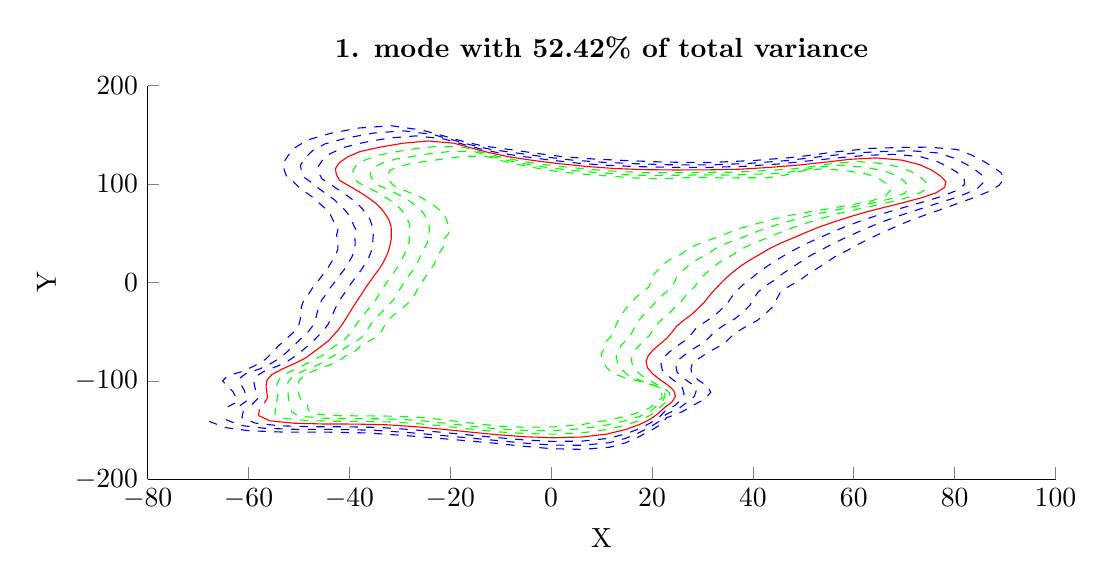
\begin{tikzpicture}

\begin{axis}[%
width=0.95092\figurewidth,
height=\figureheight,
at={(0\figurewidth,0\figureheight)},
scale only axis,
xmin=-80,
xmax=100,
xlabel={X},
ymin=-200,
ymax=200,
ylabel={Y},
title style={font=\bfseries},
title={1. mode with 52.42\% of total variance},
axis x line*=bottom,
axis y line*=left
]
\addplot [color=blue,dashed,forget plot]
  table[row sep=crcr]{%
-64.1113881531626	-126.422857227232\\
-62.3137493384501	-121.534773224667\\
-62.5526256797443	-116.293332766034\\
-63.0728549219847	-110.98018521314\\
-64.111403013549	-105.682726908696\\
-65.1322895148274	-100.031875030914\\
-64.1080439095626	-94.8104497674803\\
-61.1090411168025	-90.33972189999\\
-58.8295958909906	-84.7765929032281\\
-56.621062618512	-78.1549752094639\\
-55.3109326500943	-71.2982216786483\\
-54.0451785822157	-64.4681572170807\\
-52.6008484472825	-57.6923786737534\\
-51.1251964532574	-50.9116230843554\\
-50.0610191755853	-44.0599875699865\\
-49.7172223134401	-37.1191309253918\\
-49.6294508607351	-30.4876221921936\\
-49.4865806763933	-24.2260868148994\\
-49.0361965944735	-18.0145758621749\\
-48.0902034998486	-11.8668996644883\\
-47.2898383930681	-5.42269275190331\\
-46.3146828733534	0.690725553070188\\
-45.4186600369115	6.85423738676375\\
-44.4453716357019	12.9957785750946\\
-43.6828247766242	19.6201049927491\\
-42.7925591316775	26.6759664763406\\
-42.2893434869477	33.7738276724304\\
-42.2929514401841	40.9033038624999\\
-42.5306904422281	48.0347381765512\\
-42.215164164039	55.1473028052137\\
-43.1399711531593	62.2520905995861\\
-43.8175186741618	69.3200662393259\\
-44.8773821472101	75.5923960704164\\
-46.0958188496898	81.0627904289118\\
-47.2849655946893	86.6032465031828\\
-48.7799687820913	92.0853016737529\\
-50.1926773229734	97.5270334455254\\
-51.2514162544181	103.019816902071\\
-52.505406359378	108.498326512903\\
-52.9043463016658	114.051798955237\\
-53.1857590480468	120.8578270327\\
-52.1424654475473	128.871614371486\\
-50.7869231984063	136.863957499433\\
-48.3462903008677	144.613243273001\\
-43.7632784556929	151.448306014127\\
-38.0760626566901	156.899669468677\\
-31.6941907301334	159.182426797544\\
-25.6215339435526	154.752263983318\\
-21.5064958162697	149.125153683201\\
-17.8510640626736	143.774272712467\\
-13.6370281382769	138.742702345613\\
-8.22241503940673	135.045134317909\\
-2.97589621152903	131.182801803362\\
2.46521541859346	127.631918861494\\
8.55593505910047	125.348975265356\\
14.9677471658051	123.776088452363\\
22.6480359591807	122.218057265704\\
31.5649597008912	121.830150145465\\
40.3164634617137	123.920497372512\\
48.5660989353686	127.273172039313\\
55.9642530794155	132.373907759319\\
63.4140842903074	136.17276859077\\
68.9857411480043	137.06563826324\\
74.8289438848868	137.458024211548\\
80.497678140347	135.051565846542\\
83.3259225365914	129.465742973752\\
85.5753403547145	123.571323386359\\
87.5036686498257	117.622639474196\\
89.1775942156016	111.557729153636\\
89.7979922249149	105.225595884663\\
88.8436266197064	98.8692065058364\\
86.9224843303053	92.7257821860461\\
84.1645961294153	86.7891268580837\\
80.9568514023326	80.8783092294654\\
77.8180425112543	74.9913343219719\\
74.5239674780353	69.2198684963696\\
71.4035519556492	63.3174297815561\\
68.5650039576442	57.2552619589546\\
65.921730037945	51.1446770044502\\
63.3100045806704	45.0058087722051\\
60.9558733761274	38.8721003088333\\
58.8342087234764	32.8175330459414\\
56.4640176309109	26.8049211894389\\
54.684136723229	20.6481660800637\\
52.8443364257312	14.5229152880609\\
50.9033931859312	8.38183594041532\\
49.3366351683298	2.15210740813702\\
47.1312776959867	-4.04424070928949\\
45.3877990902005	-10.6179004353686\\
44.6296255325143	-17.70030978331\\
43.9404169584057	-24.8052686685917\\
42.4914875489309	-31.7290671870478\\
40.8721079654834	-38.6425065565061\\
38.4863249455975	-45.2928031107952\\
36.2956888269719	-51.944502245788\\
35.0103252320725	-58.733649647962\\
33.3608655968428	-64.9567805390354\\
31.2689247109958	-70.5133563116024\\
29.6665655595355	-76.0246157244469\\
28.0148262416386	-81.5907920368348\\
27.7246280580343	-87.7065677805129\\
27.9115724637363	-93.7173545678958\\
29.2780334192575	-99.6122267386532\\
30.9684451344403	-105.204106259172\\
31.6376496249636	-111.639369245924\\
30.3836726245072	-118.774045906247\\
27.9708838021748	-125.345469939367\\
26.0144789022887	-131.309562670408\\
22.8669424990321	-137.602461831795\\
21.821588953982	-144.233062467167\\
19.6540274372773	-150.708337660418\\
17.2816986468469	-157.133657648061\\
14.8379000278128	-162.840936080487\\
11.6255146635044	-167.426010238427\\
6.18167162546853	-169.648556876662\\
0.147745443773704	-168.950442183307\\
-5.60450349426934	-166.408802301064\\
-11.0949845407994	-163.421031128254\\
-16.7058794237253	-160.877311634416\\
-22.3835681934064	-158.374081318985\\
-28.9650090083777	-155.55222628904\\
-36.648433825369	-152.911218290289\\
-44.6619701957547	-152.086041473289\\
-52.7840220887422	-152.107995459061\\
-59.8823594667086	-150.721341196663\\
-64.4673179793973	-147.585298828544\\
-67.8759967645611	-141.084629166979\\
-67.3996678159056	-133.852446775627\\
};
\addplot [color=blue,dashed,forget plot]
  table[row sep=crcr]{%
-61.695953787725	-125.190245272256\\
-60.2785095200496	-120.001877428854\\
-60.499029811073	-114.537069946411\\
-60.8897946184	-109.025375623283\\
-61.5227966930159	-103.533483719334\\
-61.8663612794511	-97.8428166477487\\
-60.4962351438972	-92.52869353773\\
-57.7223996014046	-87.7474771787577\\
-55.4748746224303	-82.1951563481528\\
-53.4803691585979	-75.8313281646612\\
-52.0970672972122	-69.3045196228365\\
-50.7513035582749	-62.7968373030166\\
-49.436632050124	-56.2881836320302\\
-48.113093964095	-49.7732846043094\\
-47.1270919710259	-43.2023736575266\\
-46.6567932975192	-36.5659590044081\\
-46.3569104748883	-30.1337634944562\\
-46.0139004603166	-23.9437214493651\\
-45.4564764987152	-17.7885390958142\\
-44.5585151014238	-11.675896965039\\
-43.7824027724446	-5.34200988044179\\
-42.8480640920245	0.742082809289558\\
-41.9770437029931	6.86456060449893\\
-41.0291892967174	12.9674687481934\\
-40.2629689907632	19.4143894731556\\
-39.4647074098501	26.1699616175395\\
-38.9544445631107	32.9572466784999\\
-38.8475198696134	39.7697397192522\\
-38.9234564488773	46.583298213369\\
-38.7054308345703	53.3858219604455\\
-39.3314650166163	60.1807619792267\\
-39.8927201978543	66.9498097046236\\
-40.8241562195506	73.1647609632157\\
-41.9243984152409	78.822212560518\\
-43.1024182259622	84.5157467648869\\
-44.6232271030564	90.1386877709343\\
-46.1417130258015	95.7121346205963\\
-47.4897632465134	101.278064245981\\
-48.9700156485093	106.832128847318\\
-49.4605705436805	112.536623090926\\
-49.7141910150576	119.077165501048\\
-48.7603860531663	126.425230242263\\
-47.326226775564	133.718303652489\\
-44.8570935739479	140.729102111781\\
-40.4532863335107	146.807823225611\\
-35.1557409045002	151.748556472189\\
-29.2453570296226	154.021457357101\\
-23.5108276807479	150.327287011828\\
-19.6493287994099	144.994565694864\\
-16.0322589378425	139.841294287385\\
-11.8688156531972	135.007488703344\\
-6.65980646783072	131.329171075162\\
-1.47730350773011	127.680359530343\\
3.9163311717051	124.38778347422\\
9.84716346138721	122.15325615428\\
16.0821441618528	120.703079412113\\
23.2645650752419	119.560696493612\\
31.3500246577719	119.33467216787\\
39.2947803620665	120.941832603287\\
46.8219800041536	123.794693130317\\
53.7086636188151	128.012413289974\\
60.4865971466749	131.545258202766\\
65.7460525667162	133.074831731216\\
71.343651966029	133.793197302095\\
76.8244826431136	131.466121761116\\
79.9107159067882	126.188203024284\\
82.185109148888	120.429568148861\\
84.0345364531669	114.559347394768\\
85.5344700791069	108.571216568267\\
85.8782839517709	102.373849506604\\
84.6587148743309	96.2415215235617\\
82.3833633153951	90.4330798985261\\
79.380584431329	84.8619641249879\\
75.9987773815669	79.3543868155862\\
72.6959457588165	73.8387561658198\\
69.3887397271781	68.3205806004792\\
66.2703786821027	62.6642049838815\\
63.3886502701201	56.8719606805629\\
60.765944887241	50.9824808068347\\
58.196652052949	45.0598851679726\\
55.7664677909418	39.1298329647651\\
53.5953167256851	33.182818341779\\
51.3812401870955	27.2176597947584\\
49.5375434730962	21.170046104157\\
47.7297553910422	15.1186366033696\\
45.9378647480299	9.03181203400735\\
44.4502470750233	2.87266608017174\\
42.5858475357627	-3.26795604498727\\
41.0382330514492	-9.68633729784098\\
40.1843858497867	-16.4685438900365\\
39.4143434767987	-23.268198267261\\
38.0406812792055	-29.9306473489562\\
36.5412345499405	-36.5757637646053\\
34.4252683696823	-43.0057807380074\\
32.4882368316665	-49.4592674535257\\
31.3287871936452	-56.0329156505793\\
29.8872717247486	-62.2091721828549\\
28.0383399767467	-67.8999803410997\\
26.5125939084997	-73.5483335045536\\
25.0946225518787	-79.2331009325039\\
24.7563485766883	-85.3303208232274\\
24.9763862795279	-91.3764059415273\\
26.2131401193182	-97.3047828540775\\
27.8165250984406	-103.003828909168\\
28.8213819460206	-109.233643370574\\
28.373933141927	-115.878978703937\\
26.8662730785774	-122.167946625663\\
25.3255164833182	-128.045763824717\\
22.7282323097098	-134.168743235648\\
21.6229264589105	-140.530544096357\\
19.66282770234	-146.774556395601\\
17.3445949402049	-152.917992311551\\
14.7726599163733	-158.430466582955\\
11.4411198885411	-162.96525617167\\
6.16296256559745	-165.447949021523\\
0.236392197509329	-165.255821231626\\
-5.49160763123365	-163.202131904555\\
-10.986071274982	-160.513694214084\\
-16.4922044670727	-157.934156460588\\
-22.0169307448782	-155.349932066777\\
-28.2282027291598	-152.584303232174\\
-35.3104273503704	-150.148661605263\\
-42.7062482761098	-149.365544198106\\
-50.1969502058551	-149.35358048624\\
-56.8963117800344	-148.174200100347\\
-61.5658526577679	-145.259703148531\\
-64.5928503930024	-139.162708354565\\
-64.2119330958518	-132.216795295661\\
};
\addplot [color=blue,dashed,forget plot]
  table[row sep=crcr]{%
-59.2805194222875	-123.957633317281\\
-58.243269701649	-118.468981633041\\
-58.4454339424017	-112.780807126787\\
-58.7067343148152	-107.070566033426\\
-58.9341903724828	-101.384240529973\\
-58.6004330440747	-95.653758264583\\
-56.8844263782317	-90.2469373079798\\
-54.3357580860068	-85.1552324575255\\
-52.12015335387	-79.6137197930775\\
-50.3396756986837	-73.5076811198585\\
-48.8832019443302	-67.3108175670248\\
-47.4574285343342	-61.1255173889525\\
-46.2724156529655	-54.8839885903071\\
-45.1009914749325	-48.6349461242634\\
-44.1931647664665	-42.3447597450666\\
-43.5963642815983	-36.0127870834244\\
-43.0843700890415	-29.7799047967189\\
-42.54122024424	-23.6613560838309\\
-41.8767564029569	-17.5625023294536\\
-41.026826702999	-11.4848942655896\\
-40.2749671518211	-5.26132700898027\\
-39.3814453106955	0.793440065508928\\
-38.5354273690747	6.87488382223412\\
-37.6130069577328	12.9391589212921\\
-36.8431132049022	19.2086739535622\\
-36.1368556880227	25.6639567587384\\
-35.6195456392737	32.1406656845694\\
-35.4020882990427	38.6361755760044\\
-35.3162224555265	45.1318582501869\\
-35.1956975051017	51.6243411156772\\
-35.5229588800733	58.1094333588673\\
-35.9679217215468	64.5795531699213\\
-36.7709302918911	70.7371258560149\\
-37.752977980792	76.5816346921242\\
-38.9198708572351	82.4282470265911\\
-40.4664854240214	88.1920738681157\\
-42.0907487286295	93.8972357956671\\
-43.7281102386088	99.5363115898922\\
-45.4346249376405	105.165931181733\\
-46.0167947856952	111.021447226615\\
-46.2426229820684	117.296503969396\\
-45.3783066587853	123.97884611304\\
-43.8655303527216	130.572649805545\\
-41.3678968470282	136.844960950561\\
-37.1432942113284	142.167340437094\\
-32.2354191523103	146.597443475701\\
-26.7965233291118	148.860487916657\\
-21.4001214179431	145.902310040338\\
-17.7921617825502	140.863977706528\\
-14.2134538130113	135.908315862303\\
-10.1006031681176	131.272275061075\\
-5.09719789625471	127.613207832416\\
0.021289196068816	124.177917257324\\
5.36744692481674	121.143648086946\\
11.138391863674	118.957537043205\\
17.1965411579004	117.630070371863\\
23.8810941913031	116.90333572152\\
31.1350896146525	116.839194190276\\
38.2730972624193	117.963167834062\\
45.0778610729386	120.316214221321\\
51.4530741582148	123.650918820629\\
57.5591100030424	126.917747814762\\
62.506363985428	129.084025199191\\
67.8583600471711	130.128370392642\\
73.1512871458802	127.880677675689\\
76.4955092769851	122.910663074816\\
78.7948779430615	117.287812911362\\
80.5654042565081	111.496055315339\\
81.8913459426122	105.584703982899\\
81.9585756786268	99.5221031285463\\
80.4738031289553	93.613836541287\\
77.8442423004849	88.1403776110062\\
74.5965727332426	82.9348013918919\\
71.0407033608012	77.830464401707\\
67.5738490063788	72.6861780096677\\
64.253511976321	67.4212927045888\\
61.1372054085562	62.0109801862069\\
58.212296582596	56.4886594021711\\
55.6101597365369	50.8202846092192\\
53.0832995252277	45.11396156374\\
50.5770622057562	39.3875656206969\\
48.3564247278938	33.5481036376166\\
46.2984627432801	27.6303984000778\\
44.3909502229634	21.6919261282504\\
42.6151743563531	15.7143579186783\\
40.9723363101286	9.68178812759938\\
39.5638589817168	3.59322475220647\\
38.0404173755386	-2.49167138068506\\
36.688667012698	-8.75477416031335\\
35.739146167059	-15.236777996763\\
34.8882699951917	-21.7311278659303\\
33.5898750094802	-28.1322275108647\\
32.2103611343975	-34.5090209727044\\
30.3642117937671	-40.7187583652195\\
28.6807848363611	-46.9740326612634\\
27.647249155218	-53.3321816531967\\
26.4136778526545	-59.4615638266744\\
24.8077552424976	-65.2866043705969\\
23.3586222574638	-71.0720512846603\\
22.1744188621188	-76.875409828173\\
21.7880690953423	-82.954073865942\\
22.0412000953194	-89.0354573151589\\
23.148246819379	-94.9973389695018\\
24.664605062441	-100.803551559163\\
26.0051142670777	-106.827917495223\\
26.3641936593467	-112.983911501626\\
25.7616623549799	-118.99042331196\\
24.6365540643476	-124.781964979026\\
22.5895221203875	-130.7350246395\\
21.424263963839	-136.828025725547\\
19.6716279674027	-142.840775130784\\
17.4074912335629	-148.702326975042\\
14.7074198049339	-154.019997085423\\
11.2567251135777	-158.504502104913\\
6.14425350572636	-161.247341166383\\
0.325038951244953	-161.561200279945\\
-5.37871176819796	-159.995461508046\\
-10.8771580091646	-157.606357299913\\
-16.2785295104202	-154.99100128676\\
-21.6502932963501	-152.325782814569\\
-27.4913964499419	-149.616380175309\\
-33.9724208753718	-147.386104920238\\
-40.7505263564648	-146.645046922923\\
-47.609878322968	-146.599165513418\\
-53.9102640933602	-145.627059004031\\
-58.6643873361384	-142.934107468518\\
-61.3097040214437	-137.24078754215\\
-61.0241983757981	-130.581143815695\\
};
\addplot [color=red,solid,forget plot]
  table[row sep=crcr]{%
-56.8650850568499	-122.725021362305\\
-56.2080298832485	-116.936085837228\\
-56.3918380737305	-111.024544307164\\
-56.5236740112305	-105.115756443569\\
-56.3455840519496	-99.234997340611\\
-55.3345048086984	-93.4646998814174\\
-53.2726176125663	-87.9651810782296\\
-50.949116570609	-82.5629877362933\\
-48.7654320853097	-77.0322832380022\\
-47.1989822387695	-71.1840340750558\\
-45.6693365914481	-65.317115511213\\
-44.1635535103934	-59.4541974748884\\
-43.1081992558071	-53.479793548584\\
-42.0888889857701	-47.4966076442174\\
-41.2592375619071	-41.4871458326067\\
-40.5359352656773	-35.4596151624407\\
-39.8118297031948	-29.4260460989816\\
-39.0685400281634	-23.3789907182966\\
-38.2970363071987	-17.3364655630929\\
-37.4951383045741	-11.2938915661403\\
-36.7675315311977	-5.18064413751875\\
-35.9148265293666	0.844797321728298\\
-35.0938110351563	6.88520703996931\\
-34.1968246187483	12.9108490943909\\
-33.4232574190412	19.0029584339687\\
-32.8090039661952	25.1579518999372\\
-32.2846467154367	31.324084690639\\
-31.956656728472	37.5026114327567\\
-31.7089884621756	43.6804182870047\\
-31.685964175633	49.8628602709089\\
-31.7144527435303	56.038104738508\\
-32.0431232452393	62.209296635219\\
-32.7177043642317	68.3094907488142\\
-33.5815575463431	74.3410568237305\\
-34.737323488508	80.3407472882952\\
-36.3097437449864	86.2454599652972\\
-38.0397844314575	92.082336970738\\
-39.9664572307042	97.794558933803\\
-41.8992342267718	103.499733516148\\
-42.57301902771	109.506271362305\\
-42.7710549490792	115.515842437744\\
-41.9962272644043	121.532461983817\\
-40.4048339298793	127.426995958601\\
-37.8787001201085	132.960819789342\\
-33.8333020891462	137.526857648577\\
-29.3150974001203	141.446330479213\\
-24.3476896286011	143.699518476214\\
-19.2894151551383	141.477333068848\\
-15.9349947656904	136.733389718192\\
-12.3946486881801	131.975337437221\\
-8.33239068303789	127.537061418806\\
-3.53458932467869	123.897244589669\\
1.51988189986774	120.675474984305\\
6.81856267792838	117.899512699672\\
12.4296202659607	115.761817932129\\
18.3109381539481	114.557061331613\\
24.4976233073643	114.245974949428\\
30.9201545715332	114.343716212681\\
37.251414162772	114.984503064837\\
43.3337421417236	116.837735312326\\
49.1974846976144	119.289424351283\\
54.6316228594099	122.290237426758\\
59.2666754041399	125.093218667167\\
64.3730681283133	126.463543483189\\
69.4780916486468	124.295233590262\\
73.0803026471819	119.633123125349\\
75.4046467372349	114.146057673863\\
77.0962720598493	108.43276323591\\
78.2482218061175	102.598191397531\\
78.0388674054827	96.6703567504883\\
76.2888913835798	90.9861515590123\\
73.3051212855748	85.8476753234863\\
69.8125610351563	81.007638658796\\
66.0826293400356	76.3065419878278\\
62.4517522539411	71.5335998535156\\
59.1182842254639	66.5220048086984\\
56.0040321350098	61.3577553885324\\
53.0359428950718	56.1053581237793\\
50.4543745858329	50.6580884116037\\
47.9699469975063	45.1680379595075\\
45.3876566205706	39.6452982766288\\
43.1175327301025	33.9133889334542\\
41.2156852994646	28.0431370053973\\
39.2443569728306	22.2138061523438\\
37.500593321664	16.310079233987\\
36.0068078722273	10.3317642211914\\
34.6774708884103	4.3137834242412\\
33.4949872153146	-1.71538671638284\\
32.3391009739467	-7.82321102278573\\
31.2939064843314	-14.0050121034895\\
30.3621965135847	-20.1940574645996\\
29.1390687397548	-26.3338076727731\\
27.8794877188546	-32.4422781808036\\
26.3031552178519	-38.4317359924316\\
24.8733328410557	-44.4887978690011\\
23.9657111167908	-50.631447655814\\
22.9400839805603	-56.7139554704939\\
21.5771705082485	-62.6732284000942\\
20.2046506064279	-68.595769064767\\
19.2542151723589	-74.5177187238421\\
18.8197896139962	-80.5778269086565\\
19.106013911111	-86.6945086887905\\
20.0833535194397	-92.6898950849261\\
21.5126850264413	-98.6032742091588\\
23.1888465881348	-104.422191619873\\
24.3544541767665	-110.088844299316\\
24.6570516313825	-115.812899998256\\
23.947591645377	-121.518166133336\\
22.4508119310652	-127.301306043352\\
21.2256014687674	-133.125507354736\\
19.6804282324655	-138.906993865967\\
17.4703875269209	-144.486661638532\\
14.6421796934945	-149.609527587891\\
11.0723303386143	-154.043748038156\\
6.12554444585528	-157.046733311244\\
0.413685704980578	-157.866579328265\\
-5.26581590516227	-156.788791111537\\
-10.7682447433472	-154.699020385742\\
-16.0648545537676	-152.047846112932\\
-21.2836558478219	-149.30163356236\\
-26.7545901707241	-146.648457118443\\
-32.6344144003732	-144.623548235212\\
-38.7948044368199	-143.92454964774\\
-45.0228064400809	-143.844750540597\\
-50.924216406686	-143.079917907715\\
-55.7629220145089	-140.608511788504\\
-58.0265576498849	-135.318866729736\\
-57.8364636557443	-128.945492335728\\
};
\addplot [color=green,dashed,forget plot]
  table[row sep=crcr]{%
-54.4496506914123	-121.492409407329\\
-54.1727900648479	-115.403190041415\\
-54.3382422050592	-109.26828148754\\
-54.3406137076457	-103.160946853711\\
-53.7569777314165	-97.0857541512496\\
-52.068576573322	-91.2756414982518\\
-49.6608088469008	-85.6834248484794\\
-47.5624750552111	-79.970743015061\\
-45.4107108167494	-74.450846682927\\
-44.0582887788554	-68.8603870302531\\
-42.455471238566	-63.3234134554013\\
-40.8696784864526	-57.7828775608243\\
-39.9439828586486	-52.0755985068609\\
-39.0767864966077	-46.3582691641714\\
-38.3253103573477	-40.6295319201468\\
-37.4755062497564	-34.906443241457\\
-36.539289317348	-29.0721874012443\\
-35.5958598120867	-23.0966253527623\\
-34.7173162114404	-17.1104287967323\\
-33.9634499061493	-11.102888866691\\
-33.2600959105742	-5.09996126605723\\
-32.4482077480377	0.896154577947668\\
-31.6521947012378	6.8955302577045\\
-30.7806422797637	12.8825392674896\\
-30.0034016331802	18.7972429143752\\
-29.4811522443678	24.6519470411361\\
-28.9497477915997	30.5075036967085\\
-28.5112251579013	36.3690472895089\\
-28.1017544688248	42.2289783238226\\
-28.1762308461644	48.1013794261406\\
-27.9059466069873	53.9667761181486\\
-28.1183247689318	59.8390401005167\\
-28.6644784365722	65.8818556416134\\
-29.4101371118942	72.1004789553367\\
-30.5547761197808	78.2532475499993\\
-32.1530020659514	84.2988460624786\\
-33.9888201342856	90.2674381458089\\
-36.2048042227995	96.0528062777138\\
-38.363843515903	101.833535850563\\
-39.1292432697247	107.991095497994\\
-39.2994869160901	113.735180906092\\
-38.6141478700233	119.086077854594\\
-36.944137507037	124.281342111657\\
-34.3895033931887	129.076678628122\\
-30.523309966964	132.88637486006\\
-26.3947756479304	136.295217482725\\
-21.8988559280903	138.53854903577\\
-17.1787088923335	137.052356097358\\
-14.0778277488306	132.602801729856\\
-10.5758435633489	128.042359012139\\
-6.56417819795822	123.801847776537\\
-1.97198075310268	120.181281346923\\
3.01847460366666	117.173032711286\\
8.26967843104002	114.655377312398\\
13.7208486682474	112.566098821053\\
19.4253351499958	111.484052291363\\
25.1141524234255	111.588614177336\\
30.7052195284139	111.848238235087\\
36.2297310631248	112.005838295612\\
41.5896232105087	113.35925640333\\
46.941895237014	114.927929881938\\
51.7041357157774	117.662727038754\\
56.0269868228518	121.102412135142\\
60.8877762094555	122.798716573736\\
65.8048961514133	120.709789504836\\
69.6650960173788	116.355583175881\\
72.0144155314084	111.004302436364\\
73.6271398631905	105.369471156481\\
74.6050976696228	99.6116788121623\\
74.1191591323386	93.8186103724302\\
72.1039796382043	88.3584665767376\\
68.7660002706646	83.5549730359664\\
65.0285493370699	79.0804759257001\\
61.1245553192699	74.7826195739487\\
57.3296555015034	70.3810216973635\\
53.9830564746067	65.622716912808\\
50.8708588614633	60.7045305908578\\
47.8595892075477	55.7220568453875\\
45.2985894351288	50.4958922139882\\
42.8565944697849	45.222114355275\\
40.198251035385	39.9030309325606\\
37.8786407323112	34.2786742292918\\
36.1329078556492	28.4558756107167\\
34.0977637226979	22.7356861764371\\
32.3860122869749	16.9058005492957\\
31.041279434326	10.9817403147834\\
29.7910827951038	5.03434209627593\\
28.9495570550906	-0.939102052080629\\
27.9895349351955	-6.89164788525811\\
26.8486668016038	-12.773246210216\\
25.8361230319777	-18.6569870632689\\
24.6882624700294	-24.5353878346815\\
23.5486143033117	-30.3755353889027\\
22.2420986419367	-36.1447136196438\\
21.0658808457504	-42.0035630767388\\
20.2841730783635	-47.9307136584314\\
19.4664901084661	-53.9663471143133\\
18.3465857739994	-60.0598524295914\\
17.050678955392	-66.1194868448737\\
16.334011482599	-72.1600276195112\\
15.8515101326502	-78.2015799513711\\
16.1708277269026	-84.353560062422\\
17.0184602195004	-90.3824512003503\\
18.3607649904416	-96.4029968591543\\
20.3725789091918	-102.016465744523\\
22.3447146941863	-107.193777097006\\
23.5524409077851	-112.635376684553\\
23.2586292264065	-118.254367287645\\
22.3121017417428	-123.867587447205\\
21.0269389736959	-129.422988983926\\
19.6892284975282	-134.97321260115\\
17.5332838202788	-140.270996302023\\
14.5769395820551	-145.199058090359\\
10.887935563651	-149.582993971399\\
6.10683538598419	-152.846125456105\\
0.502332458716202	-154.171958376584\\
-5.15292004212657	-153.582120715029\\
-10.6593314775298	-151.791683471571\\
-15.8511795971151	-149.104690939105\\
-20.9170183992938	-146.277484310152\\
-26.0177838915062	-143.680534061577\\
-31.2964079253746	-141.860991550186\\
-36.839082517175	-141.204052372557\\
-42.4357345571938	-141.090335567776\\
-47.9381687200118	-140.532776811399\\
-52.8614566928795	-138.282916108491\\
-54.7434112783262	-133.396945917322\\
-54.6487289356905	-127.309840855762\\
};
\addplot [color=green,dashed,forget plot]
  table[row sep=crcr]{%
-52.0342163259747	-120.259797452353\\
-52.1375502464474	-113.870294245602\\
-52.2846463363879	-107.512018667917\\
-52.157553404061	-101.206137263854\\
-51.1683714108834	-94.9365109618881\\
-48.8026483379457	-89.0865831150861\\
-46.0490000812354	-83.4016686187292\\
-44.1758335398133	-77.3784982938288\\
-42.0559895481891	-71.8694101278517\\
-40.9175953189412	-66.5367399854504\\
-39.241605885684	-61.3297113995895\\
-37.5758034625119	-56.1115576467602\\
-36.7797664614901	-50.6714034651377\\
-36.0646840074452	-45.2199306841254\\
-35.3913831527883	-39.7719180076869\\
-34.4150772338354	-34.3532713204733\\
-33.2667489315012	-28.7183287035069\\
-32.1231795960101	-22.8142599872281\\
-31.1375961156821	-16.8843920303716\\
-30.4317615077245	-10.9118861672416\\
-29.7526602899508	-5.01927839459571\\
-28.9815889667088	0.947511834167038\\
-28.2105783673194	6.90585347543968\\
-27.3644599407792	12.8542294405884\\
-26.5835458473193	18.5915273947817\\
-26.1533005225404	24.145942182335\\
-25.6148488677627	29.690922702778\\
-25.0657935873307	35.2354831462612\\
-24.494520475474	40.7775383606405\\
-24.6664975166957	46.3398985813723\\
-24.0974404704443	51.8954474977892\\
-24.1935262926243	57.4687835658144\\
-24.6112525089127	63.4542205344127\\
-25.2387166774453	69.8599010869429\\
-26.3722287510537	76.1657478117035\\
-27.9962603869164	82.35223215966\\
-29.9378558371136	88.4525393208797\\
-32.4431512148949	94.3110536216246\\
-34.8284528050342	100.167338184978\\
-35.6854675117394	106.475919633683\\
-35.8279188831009	111.95451937444\\
-35.2320684756423	116.639693725371\\
-33.4834410841947	121.135688264712\\
-30.900306666269	125.192537466902\\
-27.2133178447817	128.245892071543\\
-23.4744538957405	131.144104486237\\
-19.4500222275795	133.377579595327\\
-15.0680026295287	132.627379125867\\
-12.2206607319709	128.47221374152\\
-8.75703843851776	124.109380587057\\
-4.79596571287855	120.066634134267\\
-0.409372181526671	116.465318104176\\
4.51706730746559	113.670590438268\\
9.72079418415166	111.411241925125\\
15.0120770705342	109.370379709978\\
20.5397321460434	108.411043251112\\
25.7306815394868	108.931253405244\\
30.4902844852945	109.352760257493\\
35.2080479634776	109.027173526387\\
39.8455042792937	109.880777494334\\
44.6863057764137	110.566435412593\\
48.7766485721449	113.035216650749\\
52.7872982415637	117.111605603118\\
57.4024842905977	119.133889664284\\
62.1317006541799	117.124345419409\\
66.2498893875756	113.078043226414\\
68.6241843255819	107.862547198865\\
70.1580076665317	102.306179077052\\
70.9619735331281	96.625166226794\\
70.1994508591946	90.9668639943721\\
67.9190678928287	85.7307815944629\\
64.2268792557544	81.2622707484465\\
60.2445376389835	77.1533131926042\\
56.1664812985042	73.2586971600695\\
52.2075587490657	69.2284435412115\\
48.8478287237496	64.7234290169176\\
45.7376855879168	60.0513057931832\\
42.6832355200236	55.3387555669957\\
40.1428042844248	50.3336960163726\\
37.7432419420635	45.2761907510425\\
35.0088454501994	40.1607635884924\\
32.6397487345199	34.6439595251294\\
31.0501304118338	28.8686142160361\\
28.9511704725651	23.2575662005305\\
27.2714312522858	17.5015218646044\\
26.0757509964247	11.6317164083755\\
24.9046947017973	5.75490076831066\\
24.4041268948665	-0.162817387778413\\
23.6399688964442	-5.96008474773049\\
22.4034271188761	-11.5414803169425\\
21.3100495503707	-17.1199166619382\\
20.2374562003041	-22.7369679965899\\
19.2177408877688	-28.3087925970019\\
18.1810420660215	-33.8576912468559\\
17.258428850445	-39.5183282844765\\
16.6026350399363	-45.2299796610487\\
15.992896236372	-51.2187387581328\\
15.1160010397503	-57.4464764590887\\
13.8967073043561	-63.6432046249805\\
13.4138077928392	-69.8023365151803\\
12.8832306513042	-75.8253329940857\\
13.2356415426942	-82.0126114360536\\
13.9535669195612	-88.0750073157746\\
15.208844954442	-94.2027195091498\\
17.5563112302489	-99.6107398691724\\
20.3349752116061	-104.298709894696\\
22.4478301841877	-109.457853370849\\
22.5696668074359	-114.990568441954\\
22.1733915524205	-120.433868851057\\
20.8282764786244	-125.720470613116\\
19.6980287625909	-131.039431336333\\
17.5961801136368	-136.055330965513\\
14.5116994706157	-140.788588592826\\
10.7035407886876	-145.122239904641\\
6.08812632611311	-148.645517600966\\
0.590979212451827	-150.477337424903\\
-5.04002417909088	-150.37545031852\\
-10.5504182117124	-148.884346557401\\
-15.6375046404625	-146.161535765277\\
-20.5503809507656	-143.253335057944\\
-25.2809776122883	-140.712611004712\\
-29.958401450376	-139.098434865161\\
-34.88336059753	-138.483555097374\\
-39.8486626743067	-138.335920594955\\
-44.9521210333376	-137.985635715083\\
-49.95999137125	-135.957320428478\\
-51.4602649067674	-131.475025104908\\
-51.4609942156367	-125.674189375796\\
};
\addplot [color=green,dashed,forget plot]
  table[row sep=crcr]{%
-49.6187819605372	-119.027185497377\\
-50.1023104280468	-112.337398449789\\
-50.2310504677166	-105.755755848294\\
-49.9744931004762	-99.2513276739971\\
-48.5797650903502	-92.7872677725266\\
-45.5367201025694	-86.8975247319205\\
-42.4371913155699	-81.119912388979\\
-40.7891920244155	-74.7862535725965\\
-38.7012682796288	-69.2879735727764\\
-37.776901859027	-64.2130929406477\\
-36.0277405328019	-59.3360093437778\\
-34.2819284385711	-54.4402377326961\\
-33.6155500643316	-49.2672084234146\\
-33.0525815182828	-44.0815922040794\\
-32.4574559482289	-38.914304095227\\
-31.3546482179145	-33.8000993994896\\
-29.9942085456544	-28.3644700057696\\
-28.6504993799334	-22.5318946216938\\
-27.5578760199239	-16.6583552640109\\
-26.9000731092997	-10.7208834677923\\
-26.2452246693273	-4.93859552313419\\
-25.5149701853799	0.998869090386408\\
-24.768962033401	6.91617669317487\\
-23.9482776017946	12.8259196136871\\
-23.1636900614583	18.3858118751882\\
-22.825448800713	23.6399373235338\\
-22.2799499439257	28.8743417088475\\
-21.62036201676	34.1019190030135\\
-20.8872864821232	39.3260983974583\\
-21.1567641872271	44.5784177366041\\
-20.2889343339013	49.8241188774298\\
-20.2687278163168	55.0985270311121\\
-20.5580265812532	61.0265854272119\\
-21.0672962429964	67.6193232185492\\
-22.1896813823266	74.0782480734076\\
-23.8395187078815	80.4056182568414\\
-25.8868915399416	86.6376404959506\\
-28.6814982069903	92.5693009655354\\
-31.2930620941655	98.5011405193931\\
-32.2416917537541	104.960743769372\\
-32.3563508501117	110.173857842789\\
-31.8499890812613	114.193309596148\\
-30.0227446613524	117.990034417768\\
-27.4111099393493	121.308396305683\\
-23.9033257225995	123.605409283027\\
-20.5541321435505	125.992991489749\\
-17.0011885270688	128.216610154883\\
-12.9572963667239	128.202402154377\\
-10.3634937151111	124.341625753183\\
-6.93823331368659	120.176402161975\\
-3.02775322779888	116.331420491998\\
1.15323639004934	112.74935486143\\
6.01566001126451	110.168148165249\\
11.1719099372633	108.167106537851\\
16.3033054728209	106.174660598902\\
21.6541291420911	105.338034210862\\
26.347210655548	106.273892633152\\
30.2753494421752	106.857282279898\\
34.1863648638304	106.048508757161\\
38.1013853480787	106.402298585338\\
42.4307163158133	106.204940943248\\
45.8491614285124	108.407706262745\\
49.5476096602756	113.120799071093\\
53.9171923717399	115.469062754831\\
58.4585051569465	113.538901333982\\
62.8346827577725	109.800503276946\\
65.2339531197553	104.720791961367\\
66.6888754698729	99.2428869976227\\
67.3188493966334	93.6386536414256\\
66.2797425860505	88.1151176163141\\
63.7341561474532	83.1030966121882\\
59.6877582408443	78.9695684609266\\
55.4605259408972	75.2261504595083\\
51.2084072777386	71.7347747461903\\
47.085461996628	68.0758653850594\\
43.7126009728925	63.8241411210272\\
40.6045123143703	59.3980809955087\\
37.5068818324995	54.955454288604\\
34.9870191337207	50.1714998187571\\
32.6298894143421	45.33026714681\\
29.8194398650138	40.4184962444242\\
27.4008567367287	35.009244820967\\
25.9673529680183	29.2813528213556\\
23.8045772224323	23.7794462246239\\
22.1568502175967	18.0972431799131\\
21.1102225585234	12.2816925019675\\
20.0183066084908	6.47545944034539\\
19.8586967346425	0.613467276523802\\
19.2904028576929	-5.02852161020286\\
17.9581874361485	-10.3097144236689\\
16.7839760687636	-15.5828462606076\\
15.7866499305787	-20.9385481584984\\
14.8868674722259	-26.242049805101\\
14.1199854901063	-31.570668874068\\
13.4509768551396	-37.0330934922143\\
12.9210970015091	-42.5292456636661\\
12.5193023642778	-48.4711304019523\\
11.8854163055012	-54.8331004885859\\
10.7427356533202	-61.1669224050872\\
10.4936041030793	-67.4446454108494\\
9.91495116995814	-73.4490860368002\\
10.3004553584857	-79.6716628096851\\
10.8886736196219	-85.7675634311989\\
12.0569249184423	-92.0024421591453\\
14.740043551306	-97.2050139938221\\
18.3252357290259	-101.403642692386\\
21.3432194605903	-106.280330057145\\
21.8807043884653	-111.726769596263\\
22.0346813630982	-117.000150254909\\
20.6296139835529	-122.017952242306\\
19.7068290276537	-127.105650071516\\
17.6590764069948	-131.839665629004\\
14.4464593591763	-136.378119095294\\
10.5191460137242	-140.661485837884\\
6.06941726624202	-144.444909745827\\
0.679625966187451	-146.782716473222\\
-4.92712831605519	-147.168779922011\\
-10.4415049458949	-145.97700964323\\
-15.42382968381	-143.218380591449\\
-20.1837435022374	-140.229185805736\\
-24.5441713330704	-137.744687947846\\
-28.6203949753773	-136.335878180135\\
-32.9276386778851	-135.763057822191\\
-37.2615907914196	-135.581505622133\\
-41.9660733466634	-135.438494618766\\
-47.0585260496205	-133.631724748465\\
-48.1771185352087	-129.553104292494\\
-48.2732594955829	-124.038537895829\\
};
\end{axis}
\end{tikzpicture}%
				\caption{Modus 1}
				\label{fig:mode1}
			\end{subfigure}
			\qquad
			\begin{subfigure}{0.45\textwidth}
				\centering
				% This file was created by matlab2tikz.
% Minimal pgfplots version: 1.3
%
%The latest updates can be retrieved from
%  http://www.mathworks.com/matlabcentral/fileexchange/22022-matlab2tikz
%where you can also make suggestions and rate matlab2tikz.
%
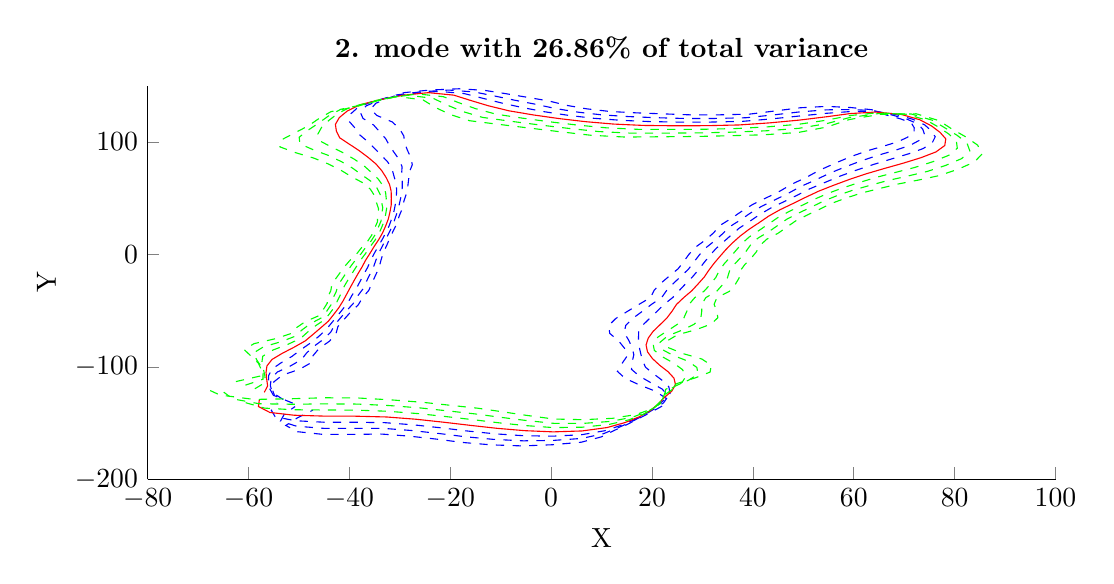
\begin{tikzpicture}

\begin{axis}[%
width=0.95092\figurewidth,
height=\figureheight,
at={(0\figurewidth,0\figureheight)},
scale only axis,
xmin=-80,
xmax=100,
xlabel={X},
ymin=-200,
ymax=150,
ylabel={Y},
title style={font=\bfseries},
title={2. mode with 26.86\% of total variance},
axis x line*=bottom,
axis y line*=left
]
\addplot [color=blue,dashed,forget plot]
  table[row sep=crcr]{%
-51.237496428345	-132.306429191379\\
-54.837895302831	-125.746779558981\\
-55.3116818197147	-119.638236139701\\
-54.9984568187473	-113.514007777185\\
-53.2918481777152	-107.476292254213\\
-49.8411444096922	-102.135661520003\\
-47.6259858748635	-96.4744565403381\\
-47.1950135148675	-90.0478566100794\\
-46.0004148884303	-83.6809247870241\\
-43.994267885798	-77.4177415502802\\
-42.681957895772	-70.9882045143104\\
-42.2715776927716	-64.2891583980012\\
-41.0470609884019	-57.8617472884963\\
-39.7796288878385	-51.4601325555301\\
-38.256875156468	-45.0658010482697\\
-37.3865275065577	-38.566825565018\\
-36.1495485340043	-32.0510039493923\\
-35.4956197976796	-25.4448600451726\\
-34.8329009195353	-18.8325032612857\\
-34.1421538554148	-12.2191533191379\\
-33.739720429412	-5.41392648976892\\
-33.2937021632905	1.24627387575211\\
-32.5986729352211	7.85883052726271\\
-31.9692254792386	14.4748922243818\\
-31.2756108181682	21.0201824649829\\
-30.5640222363394	27.4934942025311\\
-30.1275897668968	33.9934803770925\\
-29.522307633521	40.4831749797887\\
-29.2005228327323	46.9778238597622\\
-28.7215280833908	53.4908634438794\\
-28.4276814468144	60.0186869013027\\
-28.2503931047301	66.5610590684098\\
-28.1049437379711	73.0643511640457\\
-27.5315528619608	79.5661186418597\\
-27.7842087676806	85.9179952044755\\
-28.46684144728	92.2216634445774\\
-29.0129754659835	98.6199258619313\\
-29.2043513915178	105.156354784887\\
-30.0281406025594	111.489727698465\\
-31.508362280607	117.6752757445\\
-34.565672863084	123.442650469128\\
-35.7786437995241	129.065967472063\\
-34.7301376861289	134.338060334948\\
-32.1171985829835	139.084668253902\\
-29.1396804303774	143.719680301388\\
-24.0073991754087	146.027983036112\\
-18.2532925455601	147.146680112638\\
-13.186723161313	145.722581423731\\
-8.81978546142422	142.682973885501\\
-4.67931265163977	139.517051420121\\
-0.457806120812636	136.30822911191\\
3.06218815990746	132.415601842222\\
7.09770768439407	129.278938771853\\
11.757325960253	126.917920316784\\
16.8959605189458	125.742970995751\\
22.0001112380872	124.873990588642\\
27.3538273627714	124.007719645345\\
33.1633266327419	123.962149565738\\
39.2887639071291	124.586829562422\\
44.3643226691734	127.405079764588\\
49.3785732317037	130.26078728195\\
54.6393163637694	131.49295587718\\
59.4624410776368	130.444651842387\\
63.5828661861542	128.525188874977\\
66.5651529979239	123.68058896369\\
69.2661100265991	120.40889950213\\
71.4170547330251	116.737500600285\\
71.9863101605216	112.467698001653\\
71.9538226842193	108.099701476526\\
70.5759967012823	103.847897098785\\
68.6579182939331	99.9256479190053\\
66.0972409045662	96.3914593482645\\
62.7400682770787	92.1061355061849\\
59.2308388725044	86.5178280921385\\
56.1252213788145	80.5903172414704\\
53.1412691650042	74.5866859098471\\
50.5816506076375	68.3770730411122\\
47.7265519214741	62.3727027133486\\
45.3609707153151	56.1579760241694\\
42.6310140060618	50.1294262428922\\
39.9019365780968	44.1518568739769\\
37.6926410209359	37.9679949144444\\
35.6559831088956	31.7041921184617\\
33.4320176322701	25.5352459257526\\
32.2179455458339	19.0924641739258\\
30.5998410097536	12.7616420110911\\
28.6692753240574	6.47618769390898\\
27.3252221910563	-0.0175452352409367\\
26.2807138688838	-6.51107612054979\\
25.1736546993935	-12.9137828330392\\
23.4682292749759	-19.1968152787555\\
21.8215430619693	-25.4793207263126\\
20.4288136910112	-31.8818023767245\\
19.7398090448039	-38.3648715928242\\
17.4303530832423	-44.50008437191\\
15.116570125716	-50.7717559059185\\
12.8219464982875	-57.0629422949252\\
11.4144945936684	-63.3512147544528\\
11.6202312426282	-70.2572445861889\\
13.4653161395057	-77.461957443527\\
14.6564847761383	-84.1215076702343\\
15.0475489301832	-90.5259296161967\\
14.0510476182186	-97.1556742155422\\
13.1443611765652	-104.100616901956\\
14.6401691619273	-110.19201781471\\
17.1905836279883	-115.470035834047\\
20.7008103514596	-121.799986100245\\
22.8612970479534	-128.266103022013\\
22.2162549160568	-134.449445508923\\
19.8851330755916	-140.169810020679\\
17.4471398502664	-145.850154908393\\
15.0171455941603	-151.408928517207\\
12.4259563959661	-156.781571007306\\
9.99657249011388	-162.262059896417\\
5.98088962622012	-167.051399241424\\
0.326831235213677	-169.29309854708\\
-5.68491304669547	-170.358227333129\\
-11.8140217825475	-169.433369394829\\
-17.542528707116	-167.281688184281\\
-22.8428755697677	-164.246518071593\\
-28.1523463762454	-161.655377871128\\
-33.5892652629803	-159.813909566846\\
-39.3368392826369	-160.092731767597\\
-45.12818014801	-160.149215728213\\
-50.2494398755192	-157.733723842841\\
-52.6011986496772	-152.198073378327\\
-50.3551293519444	-145.567291300083\\
-47.2247251225459	-138.558468892801\\
};
\addplot [color=blue,dashed,forget plot]
  table[row sep=crcr]{%
-53.1133593045133	-129.112626581688\\
-55.2946068296368	-122.80988165173\\
-55.6717339043866	-116.767005528856\\
-55.506862549575	-110.71459066598\\
-54.3097601357933	-104.729193949679\\
-51.6722645426943	-99.2453409738078\\
-49.5081964540977	-93.6380313863019\\
-48.4463812001147	-87.5529003188173\\
-46.9220872873901	-81.4647109373501\\
-45.0625060034552	-75.3398390585387\\
-43.6777507943307	-69.0978415132779\\
-42.9022362986456	-62.6775047569636\\
-41.734107077537	-56.4010960418589\\
-40.5493822538157	-50.1389575850925\\
-39.2576626249477	-43.8729159763821\\
-38.4363300929309	-37.5310887641589\\
-37.3703089237345	-31.1760179992554\\
-36.6865932078409	-24.7562369362139\\
-35.9876127154231	-18.3338240285548\\
-35.2598153384679	-11.9107327348054\\
-34.7489907966739	-5.33616570568553\\
-34.1674102853159	1.11244835774417\\
-33.4303856351995	7.53428936483158\\
-32.7117585257418	13.9535445143848\\
-31.9914930184592	20.3477744546448\\
-31.3123494796247	26.7149801016665\\
-30.8466087497434	33.1036818149413\\
-30.333757331838	39.4896537974447\\
-30.0366780425468	45.8786886688431\\
-29.7096734474715	52.2815290528892\\
-29.523271879053	58.6918261803711\\
-29.5146364848998	65.1104715906796\\
-29.6425306133913	71.4793976923019\\
-29.5482210900882	77.8244313691499\\
-30.101913674623	84.0589125657488\\
-31.0811422131821	90.2295956181506\\
-32.0219117878081	96.4407295648669\\
-32.7917200045799	102.702422834526\\
-33.9851718106302	108.82639630436\\
-35.196581196308	114.952274283768\\
-37.3008002250824	120.800381125334\\
-37.8511716211508	126.554798975981\\
-36.6217031007124	132.034372209499\\
-34.0376990953585	137.043385432382\\
-30.7042209833003	141.655406083784\\
-25.7766319169793	144.500765517146\\
-20.2847582399071	145.99762623383\\
-15.2209538259214	144.30749863877\\
-11.1915218961796	140.699779163064\\
-7.25109133048655	137.003146759154\\
-3.08266764155439	133.384506547542\\
0.863262331712077	129.576149424704\\
5.23843242288529	126.411117509337\\
10.1110715328114	123.911784444414\\
15.4071804346174	122.415919974544\\
20.7703868767075	121.435014169632\\
26.4017593443024	120.753804746706\\
32.415602612339	120.756005114719\\
38.6096473256767	121.386054063227\\
44.0207958266901	123.882631613834\\
49.3182103870072	126.603666305061\\
54.6367518623162	128.425383060373\\
59.3971858531379	128.66084078398\\
63.8462668335406	127.837973744381\\
67.5361325481649	123.885470505881\\
70.5375075667934	120.150307376536\\
72.7462520677617	115.873686291477\\
73.6896307936308	111.122719746405\\
74.051955724852	106.265864783528\\
73.0636202693491	101.455383649353\\
71.201575990482	96.9458157990076\\
68.4998676982357	92.8768646733384\\
65.0975658631046	88.4066365570553\\
61.5147690283481	83.1140660573683\\
58.2340650038567	77.5714114454855\\
55.1336075184908	71.8984588761308\\
52.3891111167616	66.0373004902523\\
49.4963489126733	60.2835878501589\\
47.0587720054877	54.3246801533141\\
44.4106583365433	48.4756301484306\\
41.7305099255881	42.6496706748609\\
39.5009382573248	36.6164595874477\\
37.5092171724186	30.4838404141069\\
35.3694640791236	24.4280993346163\\
33.9788281377773	18.1650025272796\\
32.4021632972448	11.9516827477912\\
30.6720071788417	5.75538627068639\\
29.3818105324757	-0.583492395621573\\
28.3001762372381	-6.9484544212951\\
27.2137386277061	-13.2775259231893\\
25.7662183545122	-19.5292293407036\\
24.2607182878978	-25.7641497084661\\
22.9123717002923	-32.0686276447509\\
21.9275911024866	-38.3871597260267\\
19.9113463358468	-44.4963222042737\\
18.0662837894076	-50.724986489217\\
16.1946589923784	-56.9466133534481\\
14.8020532318617	-63.1252193029999\\
14.4817043638947	-69.7034194123816\\
15.3949491504568	-76.4805445369654\\
16.0442530554243	-82.9402807497084\\
16.4003705904925	-89.2487893070613\\
16.0618162519589	-95.6670811720035\\
15.9338024598572	-102.26816933769\\
17.4897283039964	-108.268742416431\\
19.5785404775811	-113.67630532247\\
22.0195574447673	-119.804290732915\\
23.2233952470946	-126.016790725787\\
22.2944405877263	-132.066732353733\\
20.3319558733169	-137.821709132031\\
18.1915693109994	-143.535767894251\\
15.8348929050805	-149.101506224316\\
13.1646974951423	-154.390889867501\\
10.355158439614	-159.52262261033\\
6.02910789943184	-163.716510598031\\
0.355782725135977	-165.484258807475\\
-5.54521399951774	-165.835081925932\\
-11.4654294361474	-164.521919725133\\
-17.0499706559999	-162.203740827165\\
-22.3231356624524	-159.264889901849\\
-27.6864276410716	-156.653070953567\\
-33.2709816421112	-154.750455789635\\
-39.1561610006979	-154.703337727645\\
-45.0930555787003	-154.714393999008\\
-50.4743653859081	-152.849121864466\\
-53.6551064379545	-148.33488618172\\
-52.9122721179246	-142.151149776634\\
-50.7619713002787	-135.354143373777\\
};
\addplot [color=blue,dashed,forget plot]
  table[row sep=crcr]{%
-54.9892221806816	-125.918823971996\\
-55.7513183564426	-119.872983744479\\
-56.0317859890585	-113.89577491801\\
-56.0152682804027	-107.915173554774\\
-55.3276720938715	-101.982095645145\\
-53.5033846756963	-96.3550204276126\\
-51.390407033332	-90.8016062322658\\
-49.6977488853618	-85.0579440275553\\
-47.8437596863499	-79.2484970876762\\
-46.1307441211124	-73.2619365667973\\
-44.6735436928894	-67.2074785122455\\
-43.5328949045195	-61.065851115926\\
-42.421153166672	-54.9404447952214\\
-41.3191356197929	-48.8177826146549\\
-40.2584500934274	-42.6800309044944\\
-39.4861326793041	-36.4953519632998\\
-38.5910693134646	-30.3010320491185\\
-37.8775666180021	-24.0676138272553\\
-37.1423245113109	-17.8351447958238\\
-36.377476821521	-11.6023121504728\\
-35.7582611639358	-5.25840492160214\\
-35.0411184073413	0.978622839736235\\
-34.2620983351779	7.20974820240044\\
-33.454291572245	13.4321968043878\\
-32.7073752187502	19.6753664443068\\
-32.06067672291	25.9364660008018\\
-31.56562773259	32.2138832527901\\
-31.145207030155	38.4961326151007\\
-30.8728332523612	44.7795534779239\\
-30.6978188115523	51.0721946618991\\
-30.6188623112916	57.3649654594395\\
-30.7788798650695	63.6598841129493\\
-31.1801174888115	69.894444220558\\
-31.5648893182157	76.0827440964402\\
-32.4196185815655	82.199829927022\\
-33.6954429790843	88.2375277917239\\
-35.0308481096328	94.2615332678024\\
-36.3790886176421	100.248490884164\\
-37.942203018701	106.163064910254\\
-38.884800112009	112.229272823036\\
-40.0359275870808	118.158111781539\\
-39.9236994427776	124.043630479899\\
-38.5132685152958	129.73068408405\\
-35.9581996077335	135.002102610862\\
-32.2687615362233	139.591131866181\\
-27.5458646585498	142.973547998179\\
-22.3162239342541	144.848572355022\\
-17.2551844905299	142.892415853809\\
-13.563258330935	138.716584440628\\
-9.82287000933333	134.489242098188\\
-5.70752916229614	130.460783983174\\
-1.33566349648331	126.736697007187\\
3.37915716137652	123.543296246821\\
8.46481710536991	120.905648572043\\
13.918400350289	119.088868953336\\
19.5406625153278	117.996037750622\\
25.4496913258333	117.499889848067\\
31.6678785919361	117.5498606637\\
37.9305307442244	118.185278564032\\
43.6772689842069	120.36018346308\\
49.2578475423108	122.946545328172\\
54.634187360863	125.357810243565\\
59.3319306286389	126.877029725573\\
64.1096674809269	127.150758613785\\
68.5071120984058	124.090352048071\\
71.8089051069877	119.891715250942\\
74.0754494024983	115.00987198267\\
75.3929514267401	109.777741491157\\
76.1500887654847	104.432028090529\\
75.5512438374159	99.0628701999205\\
73.7452336870309	93.9659836790099\\
70.9024944919053	89.3622699984124\\
67.4550634491304	84.7071376079256\\
63.7986991841918	79.7103040225981\\
60.3429086288989	74.5525056495006\\
57.1259458719773	69.2102318424146\\
54.1965716258857	63.6975279393923\\
51.2661459038726	58.1944729869691\\
48.7565732956603	52.4913842824589\\
46.1903026670248	46.8218340539691\\
43.5590832730793	41.1474844757448\\
41.3092354937137	35.264924260451\\
39.3624512359416	29.2634887097521\\
37.3069105259771	23.32095274348\\
35.7397107297206	17.2375408806333\\
34.204485584736	11.1417234844913\\
32.674739033626	5.03458484746379\\
31.4383988738951	-1.14943955600221\\
30.3196386055924	-7.38583272204042\\
29.2538225560188	-13.6412690133394\\
28.0642074340484	-19.8616434026516\\
26.6998935138263	-26.0489786906196\\
25.3959297095735	-32.2554529127772\\
24.1153731601692	-38.4094478592291\\
22.3923395884513	-44.4925600366374\\
21.0159974530992	-50.6782170725155\\
19.5673714864694	-56.830284411971\\
18.1896118700551	-62.899223851547\\
17.3431774851613	-69.1495942385743\\
17.3245821614078	-75.4991316304037\\
17.4320213347103	-81.7590538291824\\
17.7531922508017	-87.9716489979259\\
18.0725848856993	-94.1784881284648\\
18.7232437431493	-100.435721773425\\
20.3392874460656	-106.345467018152\\
21.9664973271738	-111.882574810893\\
23.3383045380749	-117.808595365586\\
23.5854934462358	-123.767478429561\\
22.3726262593957	-129.684019198543\\
20.7787786710421	-135.473608243384\\
18.9359987717324	-141.221380880109\\
16.6526402160007	-146.794083931424\\
13.9034385943184	-152.000208727696\\
10.7137443891142	-156.783185324243\\
6.07732617264356	-160.381621954638\\
0.384734215058277	-161.67541906787\\
-5.40551495234	-161.311936518735\\
-11.1168370897473	-159.610470055438\\
-16.5574126048837	-157.125793470049\\
-21.8033957551372	-154.283261732105\\
-27.2205089058978	-151.650764036005\\
-32.9526980212422	-149.687002012424\\
-38.9754827187589	-149.313943687692\\
-45.0579310093906	-149.279572269802\\
-50.6992908962971	-147.96451988609\\
-54.7090142262317	-144.471698985112\\
-55.4694148839048	-138.735008253185\\
-54.2992174780115	-132.149817854753\\
};
\addplot [color=red,solid,forget plot]
  table[row sep=crcr]{%
-56.8650850568499	-122.725021362305\\
-56.2080298832485	-116.936085837228\\
-56.3918380737305	-111.024544307164\\
-56.5236740112305	-105.115756443569\\
-56.3455840519496	-99.234997340611\\
-55.3345048086984	-93.4646998814174\\
-53.2726176125663	-87.9651810782296\\
-50.949116570609	-82.5629877362933\\
-48.7654320853097	-77.0322832380022\\
-47.1989822387695	-71.1840340750558\\
-45.6693365914481	-65.317115511213\\
-44.1635535103934	-59.4541974748884\\
-43.1081992558071	-53.479793548584\\
-42.0888889857701	-47.4966076442174\\
-41.2592375619071	-41.4871458326067\\
-40.5359352656773	-35.4596151624407\\
-39.8118297031948	-29.4260460989816\\
-39.0685400281634	-23.3789907182966\\
-38.2970363071987	-17.3364655630929\\
-37.4951383045741	-11.2938915661403\\
-36.7675315311977	-5.18064413751875\\
-35.9148265293666	0.844797321728298\\
-35.0938110351563	6.88520703996931\\
-34.1968246187483	12.9108490943909\\
-33.4232574190412	19.0029584339687\\
-32.8090039661952	25.1579518999372\\
-32.2846467154367	31.324084690639\\
-31.956656728472	37.5026114327567\\
-31.7089884621756	43.6804182870047\\
-31.685964175633	49.8628602709089\\
-31.7144527435303	56.038104738508\\
-32.0431232452393	62.209296635219\\
-32.7177043642317	68.3094907488142\\
-33.5815575463431	74.3410568237305\\
-34.737323488508	80.3407472882952\\
-36.3097437449864	86.2454599652972\\
-38.0397844314575	92.082336970738\\
-39.9664572307042	97.794558933803\\
-41.8992342267718	103.499733516148\\
-42.57301902771	109.506271362305\\
-42.7710549490792	115.515842437744\\
-41.9962272644043	121.532461983817\\
-40.4048339298793	127.426995958601\\
-37.8787001201085	132.960819789342\\
-33.8333020891462	137.526857648577\\
-29.3150974001203	141.446330479213\\
-24.3476896286011	143.699518476214\\
-19.2894151551383	141.477333068848\\
-15.9349947656904	136.733389718192\\
-12.3946486881801	131.975337437221\\
-8.33239068303789	127.537061418806\\
-3.53458932467869	123.897244589669\\
1.51988189986774	120.675474984305\\
6.81856267792838	117.899512699672\\
12.4296202659607	115.761817932129\\
18.3109381539481	114.557061331613\\
24.4976233073643	114.245974949428\\
30.9201545715332	114.343716212681\\
37.251414162772	114.984503064837\\
43.3337421417236	116.837735312326\\
49.1974846976144	119.289424351283\\
54.6316228594099	122.290237426758\\
59.2666754041399	125.093218667167\\
64.3730681283133	126.463543483189\\
69.4780916486468	124.295233590262\\
73.0803026471819	119.633123125349\\
75.4046467372349	114.146057673863\\
77.0962720598493	108.43276323591\\
78.2482218061175	102.598191397531\\
78.0388674054827	96.6703567504883\\
76.2888913835798	90.9861515590123\\
73.3051212855748	85.8476753234863\\
69.8125610351563	81.007638658796\\
66.0826293400356	76.3065419878278\\
62.4517522539411	71.5335998535156\\
59.1182842254639	66.5220048086984\\
56.0040321350098	61.3577553885324\\
53.0359428950718	56.1053581237793\\
50.4543745858329	50.6580884116037\\
47.9699469975063	45.1680379595075\\
45.3876566205706	39.6452982766288\\
43.1175327301025	33.9133889334542\\
41.2156852994646	28.0431370053973\\
39.2443569728306	22.2138061523438\\
37.500593321664	16.310079233987\\
36.0068078722273	10.3317642211914\\
34.6774708884103	4.3137834242412\\
33.4949872153146	-1.71538671638284\\
32.3391009739467	-7.82321102278573\\
31.2939064843314	-14.0050121034895\\
30.3621965135847	-20.1940574645996\\
29.1390687397548	-26.3338076727731\\
27.8794877188546	-32.4422781808036\\
26.3031552178519	-38.4317359924316\\
24.8733328410557	-44.4887978690011\\
23.9657111167908	-50.631447655814\\
22.9400839805603	-56.7139554704939\\
21.5771705082485	-62.6732284000942\\
20.2046506064279	-68.595769064767\\
19.2542151723589	-74.5177187238421\\
18.8197896139962	-80.5778269086565\\
19.106013911111	-86.6945086887905\\
20.0833535194397	-92.6898950849261\\
21.5126850264413	-98.6032742091588\\
23.1888465881348	-104.422191619873\\
24.3544541767665	-110.088844299316\\
24.6570516313825	-115.812899998256\\
23.947591645377	-121.518166133336\\
22.4508119310652	-127.301306043352\\
21.2256014687674	-133.125507354736\\
19.6804282324655	-138.906993865967\\
17.4703875269209	-144.486661638532\\
14.6421796934945	-149.609527587891\\
11.0723303386143	-154.043748038156\\
6.12554444585528	-157.046733311244\\
0.413685704980578	-157.866579328265\\
-5.26581590516227	-156.788791111537\\
-10.7682447433472	-154.699020385742\\
-16.0648545537676	-152.047846112932\\
-21.2836558478219	-149.30163356236\\
-26.7545901707241	-146.648457118443\\
-32.6344144003732	-144.623548235212\\
-38.7948044368199	-143.92454964774\\
-45.0228064400809	-143.844750540597\\
-50.924216406686	-143.079917907715\\
-55.7629220145089	-140.608511788504\\
-58.0265576498849	-135.318866729736\\
-57.8364636557443	-128.945492335728\\
};
\addplot [color=green,dashed,forget plot]
  table[row sep=crcr]{%
-58.7409479330182	-119.531218752613\\
-56.6647414100543	-113.999187929977\\
-56.7518901584024	-108.153313696318\\
-57.0320797420582	-102.316339332363\\
-57.3634960100278	-96.4878990360772\\
-57.1656249417004	-90.5743793352222\\
-55.1548281918005	-85.1287559241935\\
-52.2004842558561	-80.0680314450312\\
-49.6871044842695	-74.8160693883283\\
-48.2672203564267	-69.1061315833144\\
-46.6651294900068	-63.4267525101806\\
-44.7942121162673	-57.8425438338508\\
-43.7952453449421	-52.0191423019465\\
-42.8586423517473	-46.1754326737798\\
-42.2600250303868	-40.2942607607191\\
-41.5857378520505	-34.4238783615816\\
-41.0325900929249	-28.5510601488447\\
-40.2595134383246	-22.6903676093379\\
-39.4517481030864	-16.837786330362\\
-38.6127997876273	-10.9854709818078\\
-37.7768018984596	-5.10288335343536\\
-36.788534651392	0.71097180372036\\
-35.9255237351346	6.56066587753817\\
-34.9393576652515	12.3895013843939\\
-34.1391396193323	18.3305504236306\\
-33.5573312094805	24.3794377990726\\
-33.0036656982833	30.4342861284878\\
-32.768106426789	36.5090902504127\\
-32.5451436719901	42.5812830960856\\
-32.6741095397138	48.6535258799187\\
-32.8100431757689	54.7112440175764\\
-33.307366625409	60.7587091574888\\
-34.2552912396519	66.7245372770703\\
-35.5982257744706	72.5993695510207\\
-37.0550283954504	78.4816646495684\\
-38.9240445108885	84.2533921388704\\
-41.0487207532822	89.9031406736736\\
-43.5538258437663	95.3406269834416\\
-45.8562654348425	100.836402122042\\
-46.261237943411	106.783269901573\\
-45.5061823110777	112.873573093949\\
-44.068755086031	119.021293487735\\
-42.2963993444628	125.123307833152\\
-39.7992006324834	130.919536967821\\
-35.3978426420692	135.462583430973\\
-31.0843301416909	139.919112960247\\
-26.3791553229481	142.550464597406\\
-21.3236458197467	140.062250283886\\
-18.3067312004458	134.750194995756\\
-14.9664273670269	129.461432776254\\
-10.9572522037796	124.613338854438\\
-5.73351515287408	121.057792172152\\
-0.339393361641038	117.807653721789\\
5.17230825048685	114.893376827301\\
10.9408401816323	112.434766910921\\
17.0812137925684	111.118084912603\\
23.5455552888953	110.992060050789\\
30.1724305511303	111.137571761663\\
36.5722975813197	111.783727565642\\
42.9902152992404	113.315287161571\\
49.137121852918	115.632303374395\\
54.6290583579567	119.22266460995\\
59.201420179641	123.30940760876\\
64.6364687756997	125.776328352593\\
70.4490711988877	124.500115132453\\
74.3517001873762	119.374530999755\\
76.7338440719715	113.282243365056\\
78.7995926929586	107.087784980662\\
80.3463548467502	100.764354704532\\
80.5264909735495	94.2778433010561\\
78.8325490801287	88.0063194390146\\
75.7077480792443	82.3330806485603\\
72.1700586211821	77.3081397096664\\
68.3665594958793	72.9027799530576\\
64.5605958789833	68.5146940575307\\
61.1106225789504	63.8337777749822\\
57.8114926441339	59.0179828376724\\
54.8057398862711	54.0162432605895\\
52.1521758760055	48.8247925407484\\
49.7495913279878	43.514241865046\\
47.2162299680618	38.1431120775127\\
44.9258299664914	32.5618536064575\\
43.0689193629876	26.8227853010425\\
41.1818034196842	21.1066595612075\\
39.2614759136073	15.3826175873407\\
37.8091301597185	9.52180495789151\\
36.6802027431946	3.59298200101861\\
35.551575556734	-2.28133387676348\\
34.358563342301	-8.26058932353105\\
33.333990412644	-14.3687551936396\\
32.6601855931209	-20.5264715265476\\
31.5782439656833	-26.6186366549266\\
30.3630457281358	-32.6291034488299\\
28.4909372755346	-38.4540241256341\\
27.3543260936602	-44.4850357013648\\
26.9154247804823	-50.5846782391125\\
26.3127964746512	-56.5976265290167\\
24.9647291464418	-62.4472329486413\\
23.0661237276944	-68.0419438909597\\
21.18384818331	-73.5363058172805\\
20.2075578932822	-79.3965999881306\\
20.4588355714203	-85.4173683796551\\
22.0941221531801	-91.2013020413874\\
24.3021263097334	-96.7708266448929\\
26.0384057302039	-102.498916221594\\
26.7424110263593	-108.295113787739\\
25.9757987246902	-113.817204630927\\
24.3096898445182	-119.26885383711\\
22.5289976027346	-124.918592888162\\
21.6724242664927	-130.777406466089\\
20.4248576931985	-136.592606851825\\
18.2881348378411	-142.179239345641\\
15.3809207926707	-147.218846448086\\
11.4309162881145	-151.304310752069\\
6.173762719067	-153.711844667851\\
0.442637194902878	-154.057739588659\\
-5.12611685798453	-152.26564570434\\
-10.4196523969471	-149.787570716047\\
-15.5722965026515	-146.969898755816\\
-20.7639159405067	-144.320005392616\\
-26.2886714355503	-141.646150200881\\
-32.3161307795042	-139.560094458001\\
-38.6141261548809	-138.535155607788\\
-44.9876818707712	-138.409928811392\\
-51.1491419170749	-138.195315929339\\
-56.8168298027862	-136.745324591897\\
-60.5837004158651	-131.902725206288\\
-61.3737098334771	-125.741166816704\\
};
\addplot [color=green,dashed,forget plot]
  table[row sep=crcr]{%
-60.6168108091864	-116.337416142922\\
-57.1214529368601	-111.062290022726\\
-57.1119422430743	-105.282083085472\\
-57.5404854728859	-99.5169222211574\\
-58.381407968106	-93.7408007315433\\
-58.9967450747025	-87.684058789027\\
-57.0370387710348	-82.2923307701573\\
-53.4518519411033	-77.5730751537692\\
-50.6087768832293	-72.5998555386544\\
-49.3354584740839	-67.0282290915729\\
-47.6609223885655	-61.5363895091481\\
-45.4248707221413	-56.2308901928132\\
-44.4822914340772	-50.5584910553091\\
-43.6283957177245	-44.8542577033422\\
-43.2608124988665	-39.1013756888314\\
-42.6355404384237	-33.3881415607225\\
-42.253350482655	-27.6760741987078\\
-41.4504868484859	-22.0017445003793\\
-40.6064598989742	-16.3391070976311\\
-39.7304612706804	-10.6770503974753\\
-38.7860722657214	-5.02512256935196\\
-37.6622427734174	0.577146285712423\\
-36.7572364351131	6.23612471510704\\
-35.6818907117547	11.8681536743969\\
-34.8550218196233	17.6581424132925\\
-34.3056584527658	23.600923698208\\
-33.7226846811299	29.5444875663366\\
-33.579556125106	35.5155690680687\\
-33.3812988818045	41.4821479051664\\
-33.6622549037945	47.4441914889286\\
-33.9056336080075	53.3843832966448\\
-34.5716100055787	59.3081216797585\\
-35.7928781150721	65.1395838053265\\
-37.614894002598	70.857682278311\\
-39.3727333023929	76.6225820108417\\
-41.5383452767907	82.2613243124437\\
-44.0576570751069	87.7239443766091\\
-47.1411944568284	92.8866950330802\\
-49.8132966429133	98.1730707279368\\
-49.9494568591119	104.060268440841\\
-48.2413096730761	110.231303750155\\
-46.1412829076578	116.510124991653\\
-44.1879647590463	122.819619707702\\
-41.7197011448584	128.878254146301\\
-36.9623831949921	133.39830921337\\
-32.8535628832614	138.391895441281\\
-28.4106210172951	141.401410718598\\
-23.3578764843552	138.647167498925\\
-20.6784676352012	132.76700027332\\
-17.5382060458737	126.947528115288\\
-13.5821137245214	121.689616290069\\
-7.93244098106946	118.218339754635\\
-2.19866862314981	114.939832459274\\
3.52605382304532	111.887240954931\\
9.45206009730398	109.107715889714\\
15.8514894311887	107.679108493593\\
22.5934872704263	107.73814515215\\
29.4247065307274	107.931427310644\\
35.8931809998673	108.582952066447\\
42.6466884567572	109.792839010817\\
49.0767590082216	111.975182397506\\
54.6264938565036	116.155091793143\\
59.136164955142	121.525596550353\\
64.8998694230861	125.089113221997\\
71.4200507491286	124.704996674644\\
75.6230977275705	119.115938874162\\
78.0630414067081	112.418429056249\\
80.5029133260678	105.742806725414\\
82.4444878873829	98.9305180115337\\
83.0141145416163	91.8853298516239\\
81.3762067766776	85.0264873190169\\
78.1103748729138	78.8184859736342\\
74.5275562072079	73.6086407605368\\
70.650489651723	69.4990179182874\\
66.6694395040255	65.4957882615458\\
63.102960932437	61.1455507412659\\
59.6189531532579	56.6782102868125\\
56.5755368774704	51.9271283973997\\
53.8499771661781	46.9914966698932\\
51.5292356584692	41.8604457705845\\
49.0448033155531	36.6409258783967\\
46.7341272028803	31.2103182794608\\
44.9221534265106	25.6024335966877\\
43.1192498665377	19.9995129700712\\
41.0223585055507	14.4551559406944\\
39.6114524472097	8.71184569459161\\
38.6829345979789	2.87218057779602\\
37.6081638981535	-2.84728103714412\\
36.3780257106553	-8.69796762427636\\
35.3740743409567	-14.7324982837896\\
34.9581746726572	-20.8588855884957\\
34.0174191916118	-26.9034656370801\\
32.8466037374169	-32.8159287168563\\
30.6787193332173	-38.4763122588366\\
29.8353193462647	-44.4812735337286\\
29.8651384441739	-50.537908822411\\
29.6855089687422	-56.4812975875396\\
28.3522877846352	-62.2212374971884\\
25.927596848961	-67.4881187171525\\
23.1134811942611	-72.5548929107188\\
21.5953261725682	-78.2153730676047\\
21.8116572317296	-84.1402280705196\\
24.1048907869205	-89.7127089978486\\
27.0915675930254	-94.938379080627\\
28.8879648722731	-100.575640823315\\
29.130367875952	-106.501383276162\\
27.2945458179978	-111.821509263597\\
24.6717880436594	-117.019541540884\\
22.607183274404	-122.535879732972\\
22.119247064218	-128.429305577441\\
21.1692871539315	-134.278219837683\\
19.1058821487613	-139.871817052749\\
16.1196618918468	-144.82816530828\\
11.7895022376146	-148.564873465982\\
6.22198099227871	-150.376956024458\\
0.471588684825178	-150.248899849054\\
-4.98641781080679	-147.742500297143\\
-10.071060050547	-144.876121046351\\
-15.0797384515354	-141.8919513987\\
-20.2441760331914	-139.338377222872\\
-25.8227527003765	-136.64384328332\\
-31.9978471586351	-134.496640680789\\
-38.4334478729419	-133.145761567835\\
-44.9525573014616	-132.975107082187\\
-51.3740674274638	-133.310713950964\\
-57.8707375910634	-132.882137395289\\
-63.1408431818452	-128.486583682839\\
-64.9109560112099	-122.536841297679\\
};
\addplot [color=green,dashed,forget plot]
  table[row sep=crcr]{%
-62.4926736853547	-113.14361353323\\
-57.5781644636659	-108.125392115475\\
-57.4719943277463	-102.410852474626\\
-58.0488912037137	-96.7175051099518\\
-59.3993199261841	-90.9937024270095\\
-60.8278652077045	-84.7937382428318\\
-58.919249350269	-79.4559056161212\\
-54.7032196263504	-75.0781188625071\\
-51.5304492821891	-70.3836416889804\\
-50.4036965917411	-64.9503265998314\\
-48.6567152871242	-59.6460265081157\\
-46.0555293280152	-54.6192365517755\\
-45.1693375232122	-49.0978398086717\\
-44.3981490837017	-43.5330827329046\\
-44.2615999673462	-37.9084906169437\\
-43.6853430247969	-32.3524047598634\\
-43.4741108723852	-26.8010882485709\\
-42.6414602586471	-21.3131213914206\\
-41.761171694862	-15.8404278649001\\
-40.8481227537335	-10.3686298131427\\
-39.7953426329833	-4.94736178526857\\
-38.5359508954428	0.443320767704485\\
-37.5889491350914	5.91158355267591\\
-36.4244237582579	11.3468059644\\
-35.5709040199143	16.9857344029544\\
-35.0539856960511	22.8224095973434\\
-34.4417036639766	28.6546890041854\\
-34.391005823423	34.5220478857247\\
-34.217454091619	40.3830127142473\\
-34.6504002678753	46.2348570979384\\
-35.0012240402462	52.0575225757132\\
-35.8358533857484	57.8575342020282\\
-37.3304649904923	63.5546303335826\\
-39.6315622307255	69.1159950056012\\
-41.6904382093353	74.7634993721149\\
-44.1526460426928	80.269256486017\\
-47.0665933969316	85.5447480795447\\
-50.7285630698905	90.4327630827189\\
-53.7703278509841	95.5097393338311\\
-53.6376757748129	101.33726698011\\
-50.9764370350745	107.58903440636\\
-48.2138107292845	113.998956495571\\
-46.0795301736298	120.515931582253\\
-43.6402016572334	126.836971324781\\
-38.5269237479151	131.334034995766\\
-34.6227956248319	136.864677922314\\
-30.4420867116421	140.25235683979\\
-25.3921071489636	137.232084713964\\
-23.0502040699566	130.783805550883\\
-20.1099847247204	124.433623454321\\
-16.2069752452632	118.765893725701\\
-10.1313668092649	115.378887337117\\
-4.05794388465859	112.072011196758\\
1.87979939560379	108.88110508256\\
7.96328001297562	105.780664868507\\
14.621765069809	104.240132074584\\
21.6414192519573	104.484230253511\\
28.6769825103246	104.725282859625\\
35.214064418415	105.382176567252\\
42.3031616142739	106.270390860063\\
49.0163961635251	108.318061420617\\
54.6239293550504	113.087518976335\\
59.070909730643	119.741785491946\\
65.1632700704725	124.401898091401\\
72.3910302993696	124.909878216835\\
76.8944952677647	118.857346748568\\
79.3922387414447	111.554614747441\\
82.2062339591771	104.397828470166\\
84.5426209280157	97.0966813185352\\
85.5017381096832	89.4928164021917\\
83.9198644732265	82.0466551990193\\
80.5130016665833	75.3038912987082\\
76.8850537932338	69.9091418114072\\
72.9344198075668	66.0952558835172\\
68.7782831290677	62.4768824655608\\
65.0952992859235	58.4573237075497\\
61.426413662382	54.3384377359525\\
58.3453338686696	49.8380135342099\\
55.5477784563506	45.158200799038\\
53.3088799889507	40.2066496761229\\
50.8733766630443	35.1387396792806\\
48.5424244392692	29.8587829524641\\
46.7753874900336	24.3820818923329\\
45.0566963133912	18.8923663789349\\
42.7832410974941	13.5276942940481\\
41.4137747347009	7.90188643129172\\
40.6856664527632	2.15137915457343\\
39.6647522395729	-3.41322819752475\\
38.3974880790096	-9.13534592502167\\
37.4141582692693	-15.0962413739397\\
37.2561637521935	-21.1912996504437\\
36.4565944175403	-27.1882946192336\\
35.3301617466981	-33.0027539848826\\
32.8665013908999	-38.4986003920391\\
32.3163125988692	-44.4775113660923\\
32.8148521078655	-50.4911394057095\\
33.0582214628331	-56.3649686460625\\
31.7398464228285	-61.9952420457355\\
28.7890699702276	-66.9342935433452\\
25.0431142052121	-71.5734800041572\\
22.9830944518541	-77.0341461470788\\
23.1644788920389	-82.8630877613842\\
26.1156594206608	-88.2241159543099\\
29.8810088763174	-93.1059315163612\\
31.7375240143423	-98.6523654250364\\
31.5183247255447	-104.707652764585\\
28.6132929113055	-109.825813896268\\
25.0338862428006	-114.770229244659\\
22.6853689460735	-120.153166577782\\
22.5660698619433	-126.081204688794\\
21.9137166146646	-131.96383282354\\
19.9236294596815	-137.564394759857\\
16.8584029910229	-142.437484168475\\
12.1480881871148	-145.825436179895\\
6.27019926549043	-147.042067381065\\
0.500540174747478	-146.440060109449\\
-4.84671876362906	-143.219354889945\\
-9.72246770414686	-139.964671376655\\
-14.5871804004193	-136.814004041584\\
-19.7244361258762	-134.356749053128\\
-25.3568339652027	-131.641536365758\\
-31.6795635377661	-129.433186903578\\
-38.2527695910029	-127.756367527883\\
-44.9174327321519	-127.540285352981\\
-51.5989929378527	-128.426111972588\\
-58.9246453793406	-129.018950198682\\
-65.6979859478254	-125.07044215939\\
-68.4482021889427	-119.332515778655\\
};
\end{axis}
\end{tikzpicture}%
				\caption{Modus 2}
				\label{fig:mode2}
			\end{subfigure}	
			\\
			\begin{subfigure}{0.45\textwidth}
				\centering
				% This file was created by matlab2tikz.
% Minimal pgfplots version: 1.3
%
%The latest updates can be retrieved from
%  http://www.mathworks.com/matlabcentral/fileexchange/22022-matlab2tikz
%where you can also make suggestions and rate matlab2tikz.
%
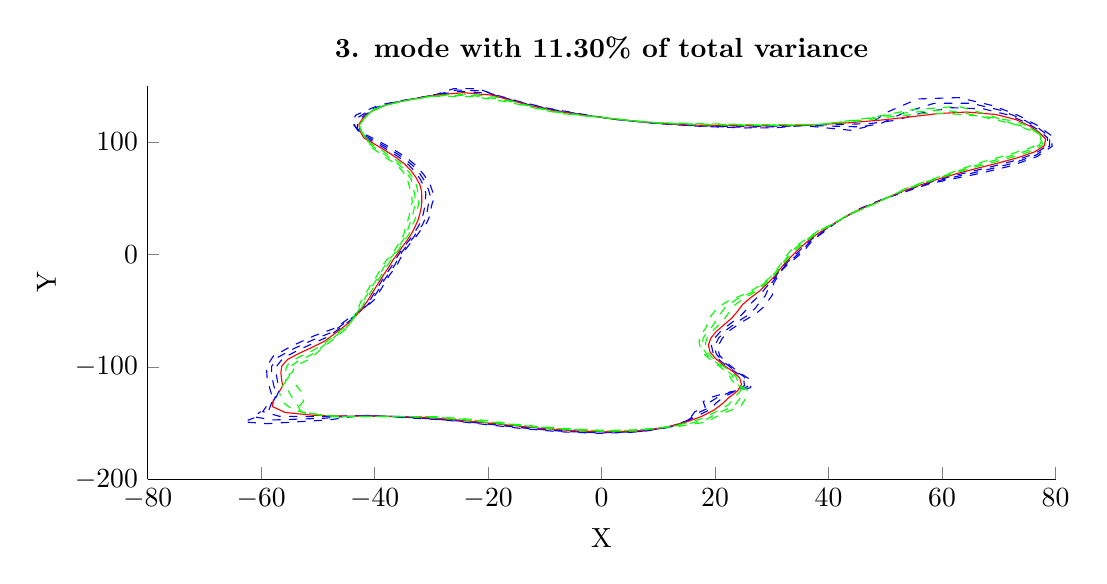
\begin{tikzpicture}

\begin{axis}[%
width=0.95092\figurewidth,
height=\figureheight,
at={(0\figurewidth,0\figureheight)},
scale only axis,
xmin=-80,
xmax=80,
xlabel={X},
ymin=-200,
ymax=150,
ylabel={Y},
title style={font=\bfseries},
title={3. mode with 11.30\% of total variance},
axis x line*=bottom,
axis y line*=left
]
\addplot [color=blue,dashed,forget plot]
  table[row sep=crcr]{%
-58.6193737057297	-138.319078758578\\
-57.9107399384524	-128.915981046782\\
-58.47129624748	-119.25995705236\\
-58.9445132537055	-109.58557369946\\
-59.0644072854577	-99.9520986208768\\
-57.8275555716103	-90.4235679551065\\
-54.5545021779963	-81.4050173407602\\
-50.7047534483931	-72.5850675944657\\
-47.2994914401819	-66.2570407498866\\
-45.9164279719243	-62.0280191429283\\
-44.7594459689413	-57.7258101973952\\
-43.4618252182764	-53.4708480541968\\
-42.2892015303312	-49.1601230274391\\
-41.0734202519053	-44.8494534194394\\
-40.0678885071914	-40.4998763957307\\
-39.5054603811978	-36.0809365066156\\
-38.8058483857283	-30.5650694873807\\
-38.0789943444387	-23.931571465913\\
-37.206335405946	-17.3188296548096\\
-36.1439815487927	-10.7230536207987\\
-35.5735062120769	-4.81802399161592\\
-34.9260031960005	1.82116607438277\\
-33.91973868042	8.42717952880677\\
-32.7923339887583	15.0072460122408\\
-31.9767951506978	20.782099370277\\
-31.0683359765831	25.7009998216671\\
-30.5590953392998	30.6612470805711\\
-30.2065592941022	35.6349331736173\\
-30.0696609889432	40.6080612441351\\
-29.8321435074974	45.5829888148673\\
-29.4697091034657	50.5759257543075\\
-29.769295613972	55.5441589904543\\
-30.2273222828117	62.1035547258962\\
-31.237217298747	70.1961934783935\\
-32.5611760788604	78.2903016673257\\
-34.4701362157951	86.2659614641084\\
-36.938776594295	94.0520708125732\\
-39.6667508257682	101.681392666724\\
-42.8132866191242	109.263273785072\\
-44.0079905951929	117.268959210521\\
-43.3173148868834	123.689457983276\\
-41.3196775124164	128.20656606514\\
-39.2221490393861	132.483484831486\\
-35.770256232064	136.247420813495\\
-32.1070875073399	139.28852693281\\
-28.9746702452029	142.323998393777\\
-26.1161195166823	147.17442574068\\
-21.8419207342336	147.325707910614\\
-18.9742615135125	142.129964388955\\
-14.485711492129	135.761407148373\\
-9.32772002045817	129.706704683994\\
-3.29602544479063	124.462729448822\\
2.91913850964772	119.552128430315\\
9.99356145951604	116.096128106465\\
17.559031144192	113.733409238556\\
25.3374153359863	112.318955725182\\
30.5952581024482	112.460867127059\\
33.2149265698656	113.573950287187\\
35.7148153387525	114.406277090702\\
39.4296488152892	112.445354105976\\
43.9199332753874	110.237167998284\\
46.4052487447671	112.982606736612\\
50.3038870146985	126.299719994194\\
55.6837171649387	138.10499208561\\
62.9467329915804	139.312669978898\\
69.04208585535	132.047551921938\\
73.4205193147727	123.523185454406\\
76.7996474718856	114.548122071115\\
79.3220391125036	105.325714327773\\
79.3824621122058	95.8946497493059\\
76.7344923974787	86.8557973912586\\
72.1499707715308	78.6350533929292\\
67.6496673323047	73.0742588931314\\
64.4038887014276	69.5160651863729\\
60.8851220447805	66.1050774763737\\
57.651882047036	62.4297015282418\\
55.1269996745152	58.3214695732443\\
52.7179278423939	54.133680389182\\
50.1048592529457	50.0000999910639\\
47.9301101606298	45.6930199135887\\
45.5240964964146	40.6015809176769\\
43.3977269499762	34.5206152012492\\
41.3193617073668	28.4038766175905\\
39.8241471975482	22.1125305800058\\
38.0859294087286	15.9338761788856\\
36.7072372456628	9.63629182058911\\
35.6981362958218	3.24666104878743\\
34.2832144990931	-3.03430508793017\\
32.8408998528227	-8.80198616657076\\
31.7881577238662	-14.1244435121467\\
31.0987417582611	-19.4905281277683\\
30.4175853184071	-24.8737353136219\\
30.0659798208083	-30.3505666609387\\
30.118075236294	-36.004922142612\\
29.3732891871812	-41.3412152521103\\
28.6388472951984	-46.5706897418993\\
27.1666980052153	-52.8729169476385\\
24.7533715247263	-60.1479408337809\\
22.6280426361926	-67.4502847877546\\
21.268915853311	-74.7792260494793\\
20.4339829208035	-82.3729991749789\\
20.7830981029974	-90.0072903964182\\
22.3075202487161	-97.4709523183579\\
24.1328579264768	-104.801652045295\\
25.9635162312329	-110.5651558444\\
26.4452884967068	-114.643952773031\\
26.233406074237	-118.624850433438\\
22.2365691993339	-122.851857841518\\
19.4829746229266	-126.855316901561\\
17.9072870400647	-130.994565779567\\
18.2652466272827	-135.846007642292\\
16.4409734614895	-139.91360480974\\
15.4943117519376	-146.409240267565\\
12.6126723458405	-153.36546172822\\
6.82527251907298	-157.900224983461\\
-0.235003798785502	-159.163294345576\\
-7.34978325259612	-157.795468776612\\
-14.1893024296669	-154.807416759301\\
-20.7497955738923	-151.126078097318\\
-27.2777519247073	-147.470709324525\\
-32.5187637363076	-145.847424322409\\
-35.7095070241004	-144.958426428643\\
-38.9145017950503	-143.627779352359\\
-42.2454093108131	-143.164393378526\\
-47.9030463681472	-147.11377810688\\
-58.9935161229781	-150.603712600925\\
-63.0730309109491	-148.95183104368\\
-61.20180981302	-145.373793219611\\
};
\addplot [color=blue,dashed,forget plot]
  table[row sep=crcr]{%
-58.0346108227698	-133.121059626487\\
-57.3431699200511	-124.922682643598\\
-57.7781435228968	-116.514819470628\\
-58.1375668395471	-108.095634614163\\
-58.1581328742883	-99.7130648607882\\
-56.9965386506397	-91.4372785972101\\
-54.127207322853	-83.5917385865834\\
-50.7862078224651	-75.9110409750749\\
-47.7881383218912	-69.8487882459251\\
-46.3439460608727	-65.0800241203041\\
-45.0627428431102	-60.2562453020012\\
-43.6957346489821	-55.465297861094\\
-42.5622007721565	-50.6000132011541\\
-41.4119098298602	-45.731838161032\\
-40.4650048587633	-40.8289662080227\\
-39.8489520093576	-35.8738293918906\\
-39.1411754915505	-30.185395024581\\
-38.4088429056803	-23.7473778833742\\
-37.5699023730302	-17.3247082909041\\
-36.5943671340532	-10.9133329359125\\
-35.9715146517838	-4.93889737358353\\
-35.2556109737892	1.49570982349795\\
-34.3110961319987	7.91318869919428\\
-33.2604975320883	14.3084470396242\\
-32.4589492401456	20.1890523915075\\
-31.6485586397871	25.5199838477571\\
-31.1342791313454	30.8821929505937\\
-30.7899251055588	36.2574925933305\\
-30.6161034800207	41.632180258425\\
-30.4500837302093	47.0096126335478\\
-30.2179569834872	52.3966520823743\\
-30.5272381577278	57.7658715387092\\
-31.057449643285	64.1722000668689\\
-32.0186640479457	71.5778145935058\\
-33.2865585487429	78.9737835409822\\
-35.0833387255255	86.2591276311713\\
-37.3057792066825	93.3954928652948\\
-39.7666529607468	100.385781422417\\
-42.5086024883401	107.342093695431\\
-43.5296667393653	114.681396594449\\
-43.1352282409487	120.964919468099\\
-41.5451940964124	125.981864704699\\
-39.6163773362172	130.797988540524\\
-36.4730708614121	135.151887138777\\
-32.682492367942	138.701303838066\\
-29.0881459635087	142.031442422256\\
-25.5266428873219	146.016123319191\\
-20.9910855412018	145.376249630025\\
-17.9611725975718	140.331106165368\\
-13.7886905574794	134.499383911322\\
-8.99594357465141	128.983490262265\\
-3.37554673808665	124.274234495771\\
2.45271963972106	119.926577281645\\
8.93522853232015	116.6972563042\\
15.8492275181149	114.409545469747\\
22.9952562753069	113.064990927325\\
28.5627131707536	113.055903067849\\
32.4500025704215	113.830538929018\\
36.227014946759	114.59901908208\\
40.731013257434	113.909481174759\\
45.6791170827964	113.254586782617\\
49.147373449648	116.085150299994\\
53.2914831445123	125.897552885185\\
58.5801674860636	134.224509218137\\
65.1238525439358	134.306857849353\\
70.388158119294	127.909408989741\\
74.0818951222601	120.397476194225\\
76.8985223345402	112.509669126046\\
78.9641000103749	104.416540017692\\
78.9345972099647	96.1532187497\\
76.5859587261791	88.2325821138432\\
72.5350209428788	81.0392607031149\\
68.3706318999219	75.7187188150196\\
64.9634689142969	71.7795574535246\\
61.4073321145007	67.914584935421\\
58.1406827731787	63.7938026217273\\
55.4193438280134	59.333564845007\\
52.8239328599532	54.7909063007145\\
50.2213643639081	50.2194294645771\\
47.9433891062553	45.518025928895\\
45.4786165377999	40.2828200373275\\
43.304328876685	34.3182064453176\\
41.2848029047327	28.2836300801927\\
39.630883789309	22.1462891041185\\
37.8908173797071	16.0592771972527\\
36.4737607878509	9.86811595412321\\
35.3579144933513	3.60236850727202\\
34.0204720711669	-2.59466563074773\\
32.673633559864	-8.47572778530909\\
31.623407310688	-14.0846330425943\\
30.8532266767023	-19.7250379067121\\
29.991413125523	-25.3604261000056\\
29.3371491201571	-31.047803834227\\
28.8464352301466	-36.8138600925519\\
27.8733037384727	-42.3904094577406\\
27.0811352357292	-47.9242757132042\\
25.7578266636637	-54.1532631219237\\
23.694637852567	-60.9897033558853\\
21.8202452929377	-67.8321128800921\\
20.5973489596603	-74.6920569409336\\
19.895918485201	-81.7746084195381\\
20.2240700390353	-88.9030298272089\\
21.5661313389573	-95.8772665738806\\
23.2594669597983	-102.735526099916\\
25.0386263502002	-108.517501102891\\
25.7483437233934	-113.125583281793\\
25.7079545932855	-117.687533621711\\
22.8069100146816	-122.407293938791\\
20.4722537256394	-127.003979948825\\
19.0133918496323	-131.704879637956\\
18.7369738290103	-136.866336383517\\
16.7841114833	-141.437957086004\\
15.2102677324566	-147.476002707674\\
12.0992250100984	-153.591557164865\\
6.59202982800041	-157.615727759389\\
-0.0187739641968085	-158.731056006472\\
-6.65512747011817	-157.459909554921\\
-13.0489498675603	-154.771284634781\\
-19.1881485671841	-151.433334102523\\
-25.2797198990788	-148.081017403804\\
-30.5973725477798	-146.114435254421\\
-34.6844761495247	-144.846800364166\\
-38.8746026756402	-143.726702784153\\
-43.1712083539024	-143.391179099216\\
-48.9101030476601	-145.769158040492\\
-57.9166514201551	-147.271978996785\\
-61.390873157261	-144.407509605699\\
-60.0800277605948	-139.897692924984\\
};
\addplot [color=blue,dashed,forget plot]
  table[row sep=crcr]{%
-57.4498479398098	-127.923040494396\\
-56.7755999016498	-120.929384240413\\
-57.0849907983136	-113.769681888896\\
-57.3306204253888	-106.605695528866\\
-57.251858463119	-99.4740311006996\\
-56.165521729669	-92.4509892393138\\
-53.6999124677096	-85.7784598324065\\
-50.867662196537	-79.2370143556841\\
-48.2767852036005	-73.4405357419637\\
-46.7714641498211	-68.13202909768\\
-45.3660397172792	-62.7866804066071\\
-43.9296440796877	-57.4597476679912\\
-42.8352000139818	-52.039903374869\\
-41.7503994078152	-46.6142229026247\\
-40.8621212103352	-41.1580560203147\\
-40.1924436375175	-35.6667222771657\\
-39.4765025973726	-29.8057205617813\\
-38.7386914669218	-23.5631843008354\\
-37.9334693401144	-17.3305869269985\\
-37.0447527193136	-11.1036122510264\\
-36.3695230914907	-5.05977075555114\\
-35.5852187515779	1.17025357261312\\
-34.7024535835775	7.3991978695818\\
-33.7286610754183	13.6096480670075\\
-32.9411033295934	19.5960054127381\\
-32.2287813029912	25.3389678738472\\
-31.709462923391	31.1031388206163\\
-31.3732909170154	36.8800520130436\\
-31.1625459710982	42.6562992727148\\
-31.0680239529212	48.4362364522284\\
-30.9662048635088	54.2173784104411\\
-31.2851807014835	59.9875840869641\\
-31.8875770037583	66.2408454078415\\
-32.8001107971444	72.9594357086181\\
-34.0119410186254	79.6572654146387\\
-35.696541235256	86.2522937982342\\
-37.67278181907	92.7389149180164\\
-39.8665550957255	99.0901701781098\\
-42.2039183575559	105.420913605789\\
-43.0513428835376	112.093833978377\\
-42.953141595014	118.240380952922\\
-41.7707106804083	123.757163344258\\
-40.0106056330483	129.112492249563\\
-37.1758854907603	134.056353464059\\
-33.2578972285441	138.114080743321\\
-29.2016216818145	141.738886450735\\
-24.9371662579615	144.857820897702\\
-20.1402503481701	143.426791349436\\
-16.9480836816311	138.53224794178\\
-13.0916696228298	133.237360674272\\
-8.66416712884465	128.260275840535\\
-3.45506803138267	124.08573954272\\
1.9863007697944	120.301026132975\\
7.87689560512426	117.298384501936\\
14.1394238920378	115.085681700938\\
20.6530972146275	113.811026129469\\
26.530168239059	113.650939008638\\
31.6850785709774	114.08712757085\\
36.7392145547655	114.791761073458\\
42.0323776995788	115.373608243543\\
47.4383008902054	116.27200556695\\
51.889498154529	119.187693863376\\
56.2790792743261	125.495385776176\\
61.4766178071885	130.344026350663\\
67.3009720962913	129.301045719807\\
71.7342303832379	123.771266057545\\
74.7432709297475	117.271766934044\\
76.9973971971948	110.471216180978\\
78.6061609082462	103.507365707611\\
78.4867323077237	96.4117877500942\\
76.4374250548794	89.6093668364277\\
72.9200711142268	83.4434680133006\\
69.0915964675391	78.3631787369078\\
65.5230491271663	74.0430497206762\\
61.9295421842209	69.7240923944683\\
58.6294834993213	65.1579037152129\\
55.7116879815116	60.3456601167697\\
52.9299378775125	55.4481322122469\\
50.3378694748705	50.4387589380904\\
47.9566680518808	45.3430319442013\\
45.4331365791853	39.9640591569782\\
43.2109308033938	34.1157976893859\\
41.2502441020987	28.163383542795\\
39.4376203810698	22.1800476282311\\
37.6957053506855	16.1846782156199\\
36.2402843300391	10.0999400876573\\
35.0176926908808	3.95807596575661\\
33.7577296432408	-2.15502617356529\\
32.5063672669054	-8.14946940404741\\
31.4586568975097	-14.0448225730419\\
30.6077115951435	-19.9595476856558\\
29.5652409326389	-25.8471168863893\\
28.6083184195059	-31.7450410075153\\
27.5747952239993	-37.6227980424918\\
26.3733182897642	-43.4396036633708\\
25.52342317626	-49.2778616845091\\
24.348955322112	-55.4336092962088\\
22.6359041804077	-61.8314658779897\\
21.0124479496828	-68.2139409724295\\
19.9257820660096	-74.6048878323878\\
19.3578540495986	-81.1762176640973\\
19.6650419750732	-87.7987692579997\\
20.8247424291985	-94.2835808294033\\
22.3860759931198	-100.669400154538\\
24.1137364691675	-106.469846361382\\
25.0513989500799	-111.607213790555\\
25.182503112334	-116.750216809984\\
23.3772508300293	-121.962730036063\\
21.4615328283523	-127.152642996089\\
20.1194966591999	-132.415193496346\\
19.2087010307379	-137.886665124742\\
17.1272495051104	-142.962309362268\\
14.9262237129755	-148.542765147782\\
11.5857776743564	-153.81765260151\\
6.35878713692784	-157.331230535317\\
0.197455870391885	-158.298817667368\\
-5.96047168764022	-157.124350333229\\
-11.9085973054538	-154.735152510262\\
-17.6265015604758	-151.740590107728\\
-23.2816878734504	-148.691325483082\\
-28.6759813592519	-146.381446186432\\
-33.6594452749489	-144.735174299689\\
-38.83470355623	-143.825626215946\\
-44.0970073969916	-143.617964819907\\
-49.917159727173	-144.424537974103\\
-56.839786717332	-143.940245392645\\
-59.708715403573	-139.863188167717\\
-58.9582457081695	-134.421592630356\\
};
\addplot [color=red,solid,forget plot]
  table[row sep=crcr]{%
-56.8650850568499	-122.725021362305\\
-56.2080298832485	-116.936085837228\\
-56.3918380737305	-111.024544307164\\
-56.5236740112305	-105.115756443569\\
-56.3455840519496	-99.234997340611\\
-55.3345048086984	-93.4646998814174\\
-53.2726176125663	-87.9651810782296\\
-50.949116570609	-82.5629877362933\\
-48.7654320853097	-77.0322832380022\\
-47.1989822387695	-71.1840340750558\\
-45.6693365914481	-65.317115511213\\
-44.1635535103934	-59.4541974748884\\
-43.1081992558071	-53.479793548584\\
-42.0888889857701	-47.4966076442174\\
-41.2592375619071	-41.4871458326067\\
-40.5359352656773	-35.4596151624407\\
-39.8118297031948	-29.4260460989816\\
-39.0685400281634	-23.3789907182966\\
-38.2970363071987	-17.3364655630929\\
-37.4951383045741	-11.2938915661403\\
-36.7675315311977	-5.18064413751875\\
-35.9148265293666	0.844797321728298\\
-35.0938110351563	6.88520703996931\\
-34.1968246187483	12.9108490943909\\
-33.4232574190412	19.0029584339687\\
-32.8090039661952	25.1579518999372\\
-32.2846467154367	31.324084690639\\
-31.956656728472	37.5026114327567\\
-31.7089884621756	43.6804182870047\\
-31.685964175633	49.8628602709089\\
-31.7144527435303	56.038104738508\\
-32.0431232452393	62.209296635219\\
-32.7177043642317	68.3094907488142\\
-33.5815575463431	74.3410568237305\\
-34.737323488508	80.3407472882952\\
-36.3097437449864	86.2454599652972\\
-38.0397844314575	92.082336970738\\
-39.9664572307042	97.794558933803\\
-41.8992342267718	103.499733516148\\
-42.57301902771	109.506271362305\\
-42.7710549490792	115.515842437744\\
-41.9962272644043	121.532461983817\\
-40.4048339298793	127.426995958601\\
-37.8787001201085	132.960819789342\\
-33.8333020891462	137.526857648577\\
-29.3150974001203	141.446330479213\\
-24.3476896286011	143.699518476214\\
-19.2894151551383	141.477333068848\\
-15.9349947656904	136.733389718192\\
-12.3946486881801	131.975337437221\\
-8.33239068303789	127.537061418806\\
-3.53458932467869	123.897244589669\\
1.51988189986774	120.675474984305\\
6.81856267792838	117.899512699672\\
12.4296202659607	115.761817932129\\
18.3109381539481	114.557061331613\\
24.4976233073643	114.245974949428\\
30.9201545715332	114.343716212681\\
37.251414162772	114.984503064837\\
43.3337421417236	116.837735312326\\
49.1974846976144	119.289424351283\\
54.6316228594099	122.290237426758\\
59.2666754041399	125.093218667167\\
64.3730681283133	126.463543483189\\
69.4780916486468	124.295233590262\\
73.0803026471819	119.633123125349\\
75.4046467372349	114.146057673863\\
77.0962720598493	108.43276323591\\
78.2482218061175	102.598191397531\\
78.0388674054827	96.6703567504883\\
76.2888913835798	90.9861515590123\\
73.3051212855748	85.8476753234863\\
69.8125610351563	81.007638658796\\
66.0826293400356	76.3065419878278\\
62.4517522539411	71.5335998535156\\
59.1182842254639	66.5220048086984\\
56.0040321350098	61.3577553885324\\
53.0359428950718	56.1053581237793\\
50.4543745858329	50.6580884116037\\
47.9699469975063	45.1680379595075\\
45.3876566205706	39.6452982766288\\
43.1175327301025	33.9133889334542\\
41.2156852994646	28.0431370053973\\
39.2443569728306	22.2138061523438\\
37.500593321664	16.310079233987\\
36.0068078722273	10.3317642211914\\
34.6774708884103	4.3137834242412\\
33.4949872153146	-1.71538671638284\\
32.3391009739467	-7.82321102278573\\
31.2939064843314	-14.0050121034895\\
30.3621965135847	-20.1940574645996\\
29.1390687397548	-26.3338076727731\\
27.8794877188546	-32.4422781808036\\
26.3031552178519	-38.4317359924316\\
24.8733328410557	-44.4887978690011\\
23.9657111167908	-50.631447655814\\
22.9400839805603	-56.7139554704939\\
21.5771705082485	-62.6732284000942\\
20.2046506064279	-68.595769064767\\
19.2542151723589	-74.5177187238421\\
18.8197896139962	-80.5778269086565\\
19.106013911111	-86.6945086887905\\
20.0833535194397	-92.6898950849261\\
21.5126850264413	-98.6032742091588\\
23.1888465881348	-104.422191619873\\
24.3544541767665	-110.088844299316\\
24.6570516313825	-115.812899998256\\
23.947591645377	-121.518166133336\\
22.4508119310652	-127.301306043352\\
21.2256014687674	-133.125507354736\\
19.6804282324655	-138.906993865967\\
17.4703875269209	-144.486661638532\\
14.6421796934945	-149.609527587891\\
11.0723303386143	-154.043748038156\\
6.12554444585528	-157.046733311244\\
0.413685704980578	-157.866579328265\\
-5.26581590516227	-156.788791111537\\
-10.7682447433472	-154.699020385742\\
-16.0648545537676	-152.047846112932\\
-21.2836558478219	-149.30163356236\\
-26.7545901707241	-146.648457118443\\
-32.6344144003732	-144.623548235212\\
-38.7948044368199	-143.92454964774\\
-45.0228064400809	-143.844750540597\\
-50.924216406686	-143.079917907715\\
-55.7629220145089	-140.608511788504\\
-58.0265576498849	-135.318866729736\\
-57.8364636557443	-128.945492335728\\
};
\addplot [color=green,dashed,forget plot]
  table[row sep=crcr]{%
-56.28032217389	-117.527002230214\\
-55.6404598648472	-112.942787434043\\
-55.6986853491473	-108.279406725432\\
-55.7167275970721	-103.625817358272\\
-55.4393096407803	-98.9959635805224\\
-54.5034878877278	-94.4784105235211\\
-52.8453227574229	-90.1519023240528\\
-51.0305709446809	-85.8889611169025\\
-49.254078967019	-80.6240307340408\\
-47.6265003277179	-74.2360390524316\\
-45.972633465617	-67.847550615819\\
-44.3974629410991	-61.4486472817856\\
-43.3811984976323	-54.9196837222989\\
-42.427378563725	-48.37899238581\\
-41.656353913479	-41.8162356448987\\
-40.8794268938371	-35.2525080477158\\
-40.1471568090169	-29.0463716361819\\
-39.3983885894049	-23.1947971357578\\
-38.6606032742829	-17.3423441991873\\
-37.9455238898346	-11.4841708812542\\
-37.1655399709046	-5.30151751948636\\
-36.2444343071554	0.519341070843473\\
-35.485168486735	6.37121621035682\\
-34.6649881620782	12.2120501217742\\
-33.905411508489	18.4099114551993\\
-33.3892266293993	24.9769359260273\\
-32.8598305074823	31.5450305606616\\
-32.5400225399287	38.1251708524698\\
-32.2554309532531	44.7045373012946\\
-32.3039043983449	51.2894840895894\\
-32.4627006235518	57.8588310665748\\
-32.801065788995	64.4310091834739\\
-33.547831724705	70.3781360897868\\
-34.3630042955418	75.7226779388428\\
-35.4627059583905	81.0242291619517\\
-36.9229462547168	86.2386261323601\\
-38.406787043845	91.4257590234596\\
-40.0663593656828	96.4989476894962\\
-41.5945500959876	101.578553426507\\
-42.0946951718823	106.918708746233\\
-42.5889683031445	112.791303922567\\
-42.2217438484003	119.307760623376\\
-40.7990622267104	125.741499667639\\
-38.5815147494566	131.865286114624\\
-34.4087069497483	136.939634553833\\
-29.4285731184261	141.153774507692\\
-23.7582129992407	142.541216054725\\
-18.4385799621065	139.527874788259\\
-14.9219058497497	134.934531494604\\
-11.6976277535305	130.71331420017\\
-8.00061423723113	126.813846997076\\
-3.61411061797472	123.708749636619\\
1.05346302994108	121.049923835635\\
5.76022975073249	118.500640897408\\
10.7198166398836	116.43795416332\\
15.9687790932687	115.303096533756\\
22.4650783756697	114.841010890218\\
30.1552305720891	114.600304854513\\
37.7636137707786	115.177245056215\\
44.6351065838684	118.301862381109\\
50.9566685050234	122.306843135617\\
57.3737475642908	125.39278099014\\
62.2542715339537	124.691051558157\\
67.2695184494382	122.583060615715\\
71.6552112010022	119.289421460717\\
74.4263749111259	115.494980193153\\
76.0660225447223	111.020348413682\\
77.1951469225039	106.394310290841\\
77.8902827039888	101.68901708745\\
77.5910025032417	96.9289257508824\\
76.1403577122801	92.3629362815968\\
73.6901714569228	88.251882633672\\
70.5335256027734	83.6520985806842\\
66.6422095529049	78.5700342549795\\
62.9739623236613	73.3431073125629\\
59.6070849516065	67.8861059021839\\
56.296376288508	62.3698506602951\\
53.1419479126312	56.7625840353117\\
50.5708796967952	50.8774178851169\\
47.9832259431318	44.9930439748138\\
45.3421766619559	39.3265373962794\\
43.0241346568113	33.7109801775226\\
41.1811264968306	27.9228904679995\\
39.0510935645915	22.2475646764564\\
37.3054812926425	16.4354802523541\\
35.7733314144154	10.5635883547255\\
34.3372490859398	4.66949088272579\\
33.2322447873884	-1.2757472592004\\
32.1718346809881	-7.49695264152405\\
31.1291560711531	-13.965201633937\\
30.1166814320259	-20.4285672435434\\
28.7128965468707	-26.8204984591568\\
27.1506570182034	-33.1395153540918\\
25.0315152117046	-39.2406739423715\\
23.3733473923472	-45.5379920746314\\
22.4079990573216	-51.985033627119\\
21.5312126390086	-57.994301644779\\
20.5184368360892	-63.5149909221986\\
19.396853263173	-68.9775971571045\\
18.5826482787082	-74.4305496152963\\
18.2817251783938	-79.9794361532157\\
18.5469858471489	-85.5902481195812\\
19.3419646096809	-91.0962093404488\\
20.6392940597628	-96.53714826378\\
22.263956707102	-102.374536878364\\
23.6575094034531	-108.570474808078\\
24.131600150431	-114.875583186529\\
24.5179324607247	-121.073602230608\\
23.440091033778	-127.449969090616\\
22.331706278335	-133.835821213126\\
20.1521554341931	-139.927322607192\\
17.8135255487313	-146.011013914797\\
14.3581356740135	-150.676290027999\\
10.5588830028723	-154.269843474801\\
5.89230175478271	-156.762236087172\\
0.629915539569271	-157.434340989161\\
-4.57116012268432	-156.453231889846\\
-9.62789218124058	-154.662888261223\\
-14.5032075470594	-152.355102118137\\
-19.2856238221935	-149.911941641639\\
-24.8331989821962	-146.915468050454\\
-31.6093835257974	-144.511922170735\\
-38.7549053174098	-144.023473079533\\
-45.9486054831702	-144.071536261288\\
-51.9312730861989	-141.735297841326\\
-54.6860573116859	-137.276778184364\\
-56.3443998961968	-130.774545291755\\
-56.714681603319	-123.469392041101\\
};
\addplot [color=green,dashed,forget plot]
  table[row sep=crcr]{%
-55.69555929093	-112.328983098123\\
-55.0728898464459	-108.949489030858\\
-55.0055326245641	-105.5342691437\\
-54.9097811829138	-102.135878272974\\
-54.5330352296109	-98.7569298204339\\
-53.6724709667571	-95.4921211656247\\
-52.4180279022796	-92.3386235698759\\
-51.1120253187529	-89.2149344975116\\
-49.7427258487282	-84.2157782300793\\
-48.0540184166663	-77.2880440298075\\
-46.275930339786	-70.3779857204249\\
-44.6313723718048	-63.4430970886828\\
-43.6541977394576	-56.3595738960139\\
-42.76586814168	-49.2613771274027\\
-42.0534702650509	-42.1453254571908\\
-41.222918521997	-35.0454009329908\\
-40.482483914839	-28.6666971733822\\
-39.7282371506465	-23.010603553219\\
-39.0241702413671	-17.3482228352818\\
-38.3959094750951	-11.6744501963681\\
-37.5635484106116	-5.42239090145396\\
-36.5740420849441	0.193884819958649\\
-35.8765259383138	5.85722538074433\\
-35.1331517054082	11.5132511491576\\
-34.3875655979368	17.8168644764298\\
-33.9694492926033	24.7959199521173\\
-33.4350142995279	31.7659764306842\\
-33.1233883513853	38.7477302721829\\
-32.8018734443306	45.7286563155845\\
-32.9218446210568	52.71610790827\\
-33.2109485035733	59.6795573946416\\
-33.5590083327507	66.6527217317289\\
-34.3779590851783	72.4467814307595\\
-35.1444510447405	77.1042990539551\\
-36.188088428273	81.7077110356082\\
-37.5361487644473	86.231792299423\\
-38.7737896562325	90.7691810761812\\
-40.1662615006615	95.2033364451894\\
-41.2898659652034	99.6573733368655\\
-41.6163713160547	104.331146130161\\
-42.4068816572098	110.066765407389\\
-42.4472604323962	117.083059262935\\
-41.1932905235415	124.056003376677\\
-39.2843293788048	130.769752439906\\
-34.9841118103504	136.352411459088\\
-29.542048836732	140.86121853617\\
-23.1687363698803	141.382913633236\\
-17.5877447690748	137.57841650767\\
-13.908816933809	133.135673271016\\
-11.0006068188808	129.45129096312\\
-7.66883779142437	126.090632575347\\
-3.69363191127074	123.520254683568\\
0.587044160014416	121.424372686966\\
4.70189682353661	119.101769095144\\
9.01001301380647	117.114090394511\\
13.6266200325893	116.0491317359\\
20.4325334439751	115.436046831007\\
29.3903065726449	114.856893496345\\
38.2758133787851	115.369987047594\\
45.9364710260132	119.765989449892\\
52.7158523124324	125.32426191995\\
60.1158722691717	128.495324553521\\
65.2418676637676	124.288884449148\\
70.1659687705631	118.702577748242\\
73.8323307533577	114.283609331172\\
75.7724471750699	111.356837260956\\
76.7273983522097	107.894639153501\\
77.2940217851585	104.355857345773\\
77.53234360186	100.779842777369\\
77.1431376010007	97.1874947512765\\
75.9918240409805	93.7397210041814\\
74.0752216282708	90.6560899438577\\
71.2544901703906	86.2965585025725\\
67.2017897657742	80.8335265221311\\
63.4961723933816	75.1526147716103\\
60.0958856777491	69.2502069956694\\
56.5887204420061	63.3819459320577\\
53.2479529301905	57.4198099468441\\
50.6873848077576	51.0967473586302\\
47.9965048887573	44.8180499901201\\
45.2966967033412	39.00777651593\\
42.9307365835201	33.5085714215909\\
41.1465676941965	27.8026439306018\\
38.8578301563523	22.281323200569\\
37.1103692636209	16.5608812707213\\
35.5398549566036	10.7954124882596\\
33.9970272834693	5.02519834121039\\
32.9695023594622	-0.836107802017962\\
32.0045683880294	-7.17069426026238\\
30.9644056579749	-13.9253911643846\\
29.8711663504671	-20.6630770224872\\
28.2867243539866	-27.3071892455406\\
26.4218263175522	-33.8367525273801\\
23.7598752055572	-40.0496118923114\\
21.8733619436388	-46.5871862802617\\
20.8502869978524	-53.3386195984239\\
20.122341297457	-59.2746478190641\\
19.4597031639299	-64.356753444303\\
18.589055919918	-69.359425249442\\
17.9110813850575	-74.3433805067506\\
17.7436607427914	-79.381045397775\\
17.9879577831867	-84.485987550372\\
18.6005756999221	-89.5025235959715\\
19.7659030930843	-94.4710223184013\\
21.3390668260693	-100.326882136855\\
22.9605646301397	-107.05210531684\\
23.6061486694796	-113.938266374801\\
25.0882732760724	-120.629038327881\\
24.4293701364909	-127.59863213788\\
23.4378110879026	-134.546135071516\\
20.6238826359207	-140.947651348417\\
18.1566635705418	-147.535366191061\\
14.0740916545325	-151.743052468107\\
10.0454356671302	-154.495938911446\\
5.65905906371014	-156.4777388631\\
0.846145374157964	-157.002102650057\\
-3.87650434020637	-156.117672668154\\
-8.48753961913399	-154.626756136703\\
-12.9415605403512	-152.662358123342\\
-17.287591796565	-150.522249720917\\
-22.9118077936683	-147.182478982466\\
-30.5843526512217	-144.400296106258\\
-38.7150061979996	-144.122396511327\\
-46.8744045262595	-144.298321981978\\
-52.9383297657118	-140.390677774938\\
-53.6091926088628	-133.945044580224\\
-54.6622421425088	-126.230223853774\\
-55.5928995508938	-117.993291746473\\
};
\addplot [color=green,dashed,forget plot]
  table[row sep=crcr]{%
-55.1107964079701	-107.130963966031\\
-54.5053198280446	-104.956190627674\\
-54.3123798999809	-102.789131561967\\
-54.1028347687555	-100.645939187677\\
-53.6267608184416	-98.5178960603453\\
-52.8414540457865	-96.5058318077284\\
-51.9907330471362	-94.525344815699\\
-51.1934796928248	-92.5409078781208\\
-50.2313727304375	-87.8075257261179\\
-48.4815365056147	-80.3400490071833\\
-46.5792272139549	-72.9084208250308\\
-44.8652818025104	-65.43754689558\\
-43.9271969812829	-57.7994640697288\\
-43.1043577196349	-50.1437618689953\\
-42.4505866166228	-42.4744152694828\\
-41.5664101501568	-34.8382938182658\\
-40.8178110206612	-28.2870227105825\\
-40.058085711888	-22.8264099706802\\
-39.3877372084513	-17.3541014713762\\
-38.8462950603556	-11.864729511482\\
-37.9615568503185	-5.54326428342157\\
-36.9036498627328	-0.131571430926176\\
-36.2678833898925	5.34323455113184\\
-35.6013152487382	10.8144521765409\\
-34.8697196873846	17.2238174976604\\
-34.5496719558074	24.6149039782074\\
-34.0101980915735	31.9869223007068\\
-33.7067541628419	39.3702896918961\\
-33.3483159354081	46.7527753298744\\
-33.5397848437686	54.1427317269505\\
-33.9591963835948	61.5002837227084\\
-34.3169508765065	68.8744342799838\\
-35.2080864456516	74.5154267717321\\
-35.9258977939392	78.4859201690675\\
-36.9134708981556	82.3911929092647\\
-38.1493512741777	86.2249584664859\\
-39.14079226862	90.1126031289028\\
-40.2661636356402	93.9077252008825\\
-40.9851818344193	97.7361932472243\\
-41.138047460227	101.743583514089\\
-42.2247950112751	107.342226892212\\
-42.6727770163922	114.858357902494\\
-41.5875188203725	122.370507085715\\
-39.987144008153	129.674218765188\\
-35.5595166709525	135.765188364344\\
-29.6555245550378	140.568662564649\\
-22.5792597405199	140.224611211748\\
-16.736909576043	135.628958227082\\
-12.8957280178683	131.336815047429\\
-10.3035858842312	128.189267726069\\
-7.33706134561762	125.367418153617\\
-3.77315320456676	123.331759730517\\
0.120625290087754	121.798821538296\\
3.64356389634072	119.70289729288\\
7.30020938772935	117.790226625702\\
11.2844609719099	116.795166938044\\
18.3999885122804	116.031082771797\\
28.6253825732008	115.113482138176\\
38.7880129867916	115.562729038972\\
47.237835468158	121.230116518675\\
54.4750361198414	128.341680704283\\
62.8579969740527	131.597868116903\\
68.2294637935814	123.886717340139\\
73.062419091688	114.822094880768\\
76.0094503057132	109.277797201627\\
77.1185194390139	107.21869432876\\
77.3887741596971	104.76892989332\\
77.392896647813	102.317404400704\\
77.1744044997313	99.8706684672888\\
76.6952726987597	97.4460637516706\\
75.8432903696809	95.1165057267659\\
74.4602717996187	93.0602972540434\\
71.9754547380078	88.9410184244607\\
67.7613699786435	83.0970187892827\\
64.0183824631018	76.9621222306576\\
60.5846864038917	70.6143080891549\\
56.8810645955043	64.3940412038204\\
53.3539579477498	58.0770358583765\\
50.80388991872	51.3160768321434\\
48.0097838343828	44.6430560054264\\
45.2512167447266	38.6890156355806\\
42.8373385102289	33.3061626656593\\
41.1120088915625	27.682397393204\\
38.6645667481131	22.3150817246817\\
36.9152572345994	16.6862822890884\\
35.3063784987918	11.0272366217937\\
33.6568054809988	5.38090579969498\\
32.7067599315361	-0.39646834483552\\
31.8373020950707	-6.8444358790007\\
30.7996552447966	-13.8855806948322\\
29.6256512689083	-20.8975868014309\\
27.8605521611025	-27.7938800319243\\
25.692995616901	-34.5339897006684\\
22.4882351994098	-40.8585498422513\\
20.3733764949303	-47.6363804858919\\
19.2925749383832	-54.6922055697288\\
18.7134699559053	-60.5549939933492\\
18.4009694917706	-65.1985159664075\\
17.7812585766631	-69.7412533417795\\
17.2395144914068	-74.2562113982049\\
17.205596307189	-78.7826546423342\\
17.4289297192246	-83.3817269811628\\
17.8591867901633	-87.9088378514942\\
18.8925121264058	-92.4048963730225\\
20.4141769450366	-98.2792273953463\\
22.2636198568263	-105.533735825602\\
23.0806971885281	-113.000949563074\\
25.6586140914201	-120.184474425153\\
25.4186492392037	-127.747295185144\\
24.5439158974701	-135.256448929906\\
21.0956098376482	-141.967980089642\\
18.4998015923522	-149.059718467325\\
13.7900476350515	-152.809814908216\\
9.53198833138817	-154.722034348091\\
5.42581637263758	-156.193241639028\\
1.06237520874666	-156.569864310953\\
-3.18184855772842	-155.782113446462\\
-7.3471870570274	-154.590624012184\\
-11.3799135336429	-152.969614128547\\
-15.2895597709366	-151.132557800196\\
-20.9904166051405	-147.449489914477\\
-29.559321776646	-144.288670041781\\
-38.6751070785895	-144.221319943121\\
-47.8002035693487	-144.525107702668\\
-53.9453864452248	-139.046057708549\\
-52.5323279060397	-130.613310976084\\
-52.9800843888207	-121.685902415793\\
-54.4711174984686	-112.517191451845\\
};
\end{axis}
\end{tikzpicture}%
				\caption{Modus 3}
				\label{fig:mode3}
			\end{subfigure}
			\qquad
			\begin{subfigure}{0.45\textwidth}
				\centering
				% This file was created by matlab2tikz.
% Minimal pgfplots version: 1.3
%
%The latest updates can be retrieved from
%  http://www.mathworks.com/matlabcentral/fileexchange/22022-matlab2tikz
%where you can also make suggestions and rate matlab2tikz.
%
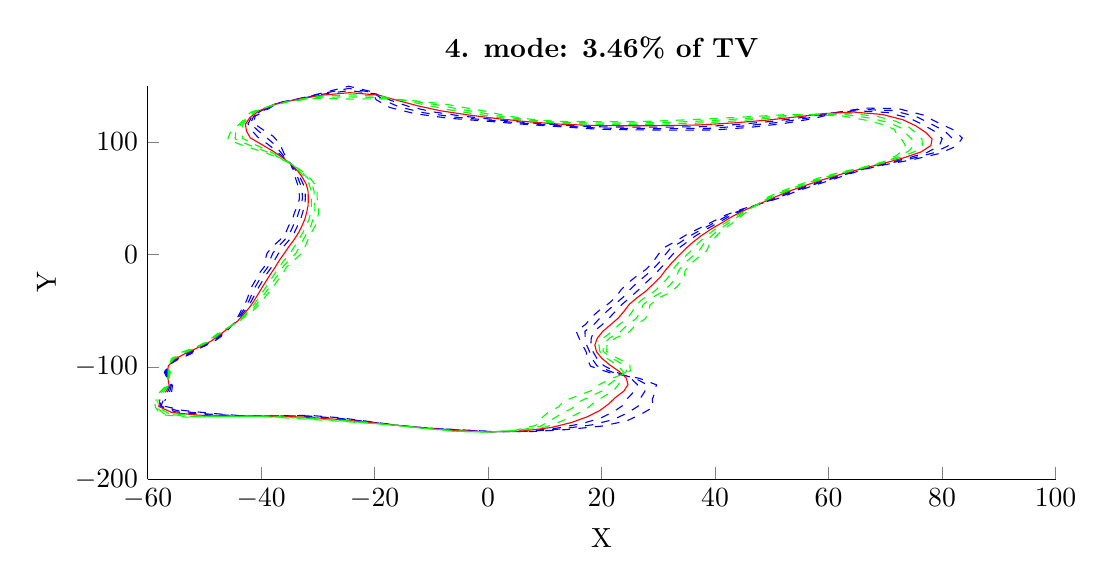
\begin{tikzpicture}

\begin{axis}[%
width=0.95092\figurewidth,
height=\figureheight,
at={(0\figurewidth,0\figureheight)},
scale only axis,
xmin=-60,
xmax=100,
xlabel={X},
ymin=-200,
ymax=150,
ylabel={Y},
title style={font=\bfseries},
title={4. mode: 3.46\% of TV},
axis x line*=bottom,
axis y line*=left
]
\addplot [color=blue,dashed,forget plot]
  table[row sep=crcr]{%
-55.7671478581589	-122.321913351108\\
-55.6278150195823	-116.615739101658\\
-56.4477919720177	-110.880391236616\\
-57.0461645834889	-105.120570922306\\
-56.5853228149416	-99.3743655577022\\
-54.832584111751	-93.9927788599231\\
-52.4661006595763	-88.7443004097182\\
-50.6893162582924	-83.2505413024613\\
-48.3774989466764	-77.7828915707806\\
-46.6931196289506	-71.8441556526405\\
-45.605738901637	-65.7493571159346\\
-44.5354818916976	-59.6601074623189\\
-43.8672509860657	-53.5001806373197\\
-43.2648489721604	-47.3308200598009\\
-42.5648492892032	-41.2009528131994\\
-42.1307802409872	-35.0533160405411\\
-41.6714763935451	-28.9639855906577\\
-40.980538970988	-22.9518346354312\\
-40.3402798419909	-16.9558921546429\\
-39.4219890972119	-10.9811073811457\\
-39.2819784302045	-4.91196512796911\\
-38.9395600952014	1.08454038162261\\
-37.9365998071035	7.05691172428768\\
-36.646628064849	12.9537994820837\\
-35.6667351769732	18.9950998719473\\
-35.1523585702267	25.1825776910809\\
-34.4715296301277	31.3656585935823\\
-34.077809652189	37.5608383136098\\
-33.4825891773774	43.7484428439088\\
-33.2400887883156	49.9550671492517\\
-33.2953518929503	56.1538896409896\\
-33.5874773215985	62.3489179707207\\
-33.9867609383386	68.4827678744262\\
-34.3465211139525	74.5733909849328\\
-34.8444815256729	80.6571135952166\\
-35.69442475793	86.7144585131018\\
-36.2380226855839	92.8536753162924\\
-36.7860815107187	98.979266011445\\
-37.8903248787309	104.998291519216\\
-39.7177414394695	110.894220210656\\
-41.400232477308	116.760175793093\\
-41.0301204912834	122.833635905796\\
-38.9227198826552	128.650621006345\\
-37.0882695894333	134.647879754848\\
-32.7465312707264	139.035493726877\\
-28.6227205799706	144.142270561673\\
-24.5763128446133	149.413540068921\\
-20.5600641895921	144.640390227893\\
-19.7186717492652	137.390274725925\\
-17.3119663734036	130.492807895694\\
-12.8701555370302	124.991711605079\\
-6.99247805181616	120.966213464162\\
-0.253287557602013	118.365342023111\\
6.25106949709879	115.632304960374\\
12.8966178362376	113.378181745622\\
19.6247350728654	111.10268314654\\
26.4556439098168	110.606186861246\\
33.0722310810186	110.407465367564\\
39.7579251615119	110.478221352818\\
46.0636322547803	112.806698412262\\
51.9255388907054	116.132741041483\\
57.2240059074804	120.53627513553\\
61.5481585556242	126.023102010047\\
66.2177425297651	129.996319050366\\
72.2685641761597	129.480880331779\\
76.6358252140077	123.876604021438\\
79.2407256425268	117.080778371209\\
82.1261164019117	110.376468634383\\
83.5710655984914	103.329036926173\\
82.5635426518981	96.1809922449125\\
79.4702666211068	89.5263453126273\\
74.6621940792365	83.9464653644022\\
69.8060481902468	79.5127652387231\\
66.0408405353527	75.2112485894343\\
63.0052265831773	70.3094975229699\\
60.0165446900388	65.3738923162652\\
56.9750163012031	60.4558971017298\\
54.0492631729989	55.4800291103163\\
51.5535202671159	50.300488404952\\
48.3319817462601	45.4526400863397\\
44.9018990922493	40.4252413887496\\
41.863133369803	34.8483239083195\\
39.5452265128931	28.9960778441368\\
37.2518412500286	23.1619167426311\\
34.9386138851473	17.3014807642325\\
32.9686852489067	11.3316103660564\\
30.8078108566926	5.39652786063002\\
29.9051654572101	-0.809483617677981\\
29.0306368620779	-7.05532130958782\\
27.8731819122272	-13.2361148847907\\
26.1913755388832	-19.3170079880804\\
24.6756052757016	-25.4398454243971\\
23.4193606376008	-31.6148170712085\\
22.58388428785	-37.7834613590749\\
21.2308355754016	-43.8551093091569\\
19.5758556107709	-49.9372823095955\\
18.197968506294	-56.0701397471498\\
17.2038782221054	-62.2779790398612\\
15.5120566579522	-68.2614395088515\\
16.0380911482394	-74.5747211749134\\
16.6758422318416	-80.8929236011453\\
17.315572040998	-87.0598721625458\\
17.4828738419463	-93.1945522858675\\
18.0512687213708	-99.4509730122356\\
21.3145854487483	-105.089642641894\\
26.671690847947	-110.286297737295\\
29.6632982105476	-116.013021644582\\
29.4167097570331	-122.40448204076\\
28.9390147167332	-129.07110336665\\
29.0604565628521	-136.005354643069\\
26.9656918188967	-142.132870134174\\
24.4529889219434	-148.070616107286\\
20.049328386216	-152.749896313743\\
13.7712049822315	-155.870958510231\\
7.61740337308566	-157.613497490227\\
1.40485592192719	-157.626739270639\\
-4.71759986924361	-156.075391163665\\
-10.5467903138167	-154.475223796544\\
-16.0431049161759	-151.944169746529\\
-21.070254969413	-148.562964561615\\
-26.119409156266	-145.313694780192\\
-31.506634400997	-143.20017846602\\
-37.4817972173019	-143.70780723422\\
-43.3280281274039	-143.562292868944\\
-48.7917471045956	-141.395492305958\\
-53.7551542947874	-138.800527635889\\
-57.4456246874674	-134.590110465091\\
-56.8258990376135	-128.764521293749\\
};
\addplot [color=blue,dashed,forget plot]
  table[row sep=crcr]{%
-56.1331269243892	-122.456282688173\\
-55.8212199741377	-116.722521346848\\
-56.4291406725886	-110.928442260132\\
-56.8720010594027	-105.11896609606\\
-56.5054098939443	-99.3279094853385\\
-54.9998910107335	-93.8167525337546\\
-52.7349396439063	-88.4845939658886\\
-50.7759163623979	-83.0213567804053\\
-48.5068099928875	-77.5326887931878\\
-46.8617404988902	-71.6241151267789\\
-45.6269381315741	-65.6052765810274\\
-44.4115057645962	-59.5914707998421\\
-43.6142337426461	-53.4933849410745\\
-42.8728623100303	-47.3860825879397\\
-42.1296453801045	-41.2963504863352\\
-41.5991652492173	-35.1887490811743\\
-41.0515941634283	-29.118005760099\\
-40.3432059900465	-23.0942199963864\\
-39.6591986637268	-17.0827499574596\\
-38.779705499666	-11.0853687761439\\
-38.4438294638689	-5.00152479781899\\
-37.9313155732565	1.00462602832451\\
-36.9890035497878	6.99967682951489\\
-35.8300269161488	12.9394826861861\\
-34.9189092576625	18.9977193926211\\
-34.3712403688829	25.174369094033\\
-33.742568658564	31.3518006259345\\
-33.3707586776167	37.5414293533254\\
-32.8913889389768	43.7257679916075\\
-32.7220472507548	49.9243315231374\\
-32.7683855098103	56.1152946734957\\
-33.0726926294788	62.3023775255535\\
-33.563742080303	68.4250088325555\\
-34.0915332580827	74.495946264532\\
-34.8087621799512	80.5516581595761\\
-35.8995310869488	86.5581256638336\\
-36.8386099342084	92.5965625344409\\
-37.8462067507139	98.584363652231\\
-39.2266279947445	104.49877218486\\
-40.6695006355496	110.431570594539\\
-41.8571733012318	116.345398007976\\
-41.3521560823237	122.399911265136\\
-39.4167578983966	128.24274599043\\
-37.3517464329917	134.085526433012\\
-33.1087882101996	138.53261503411\\
-28.8535128533538	143.24362386752\\
-24.5001051059426	147.508866204685\\
-20.1365145114408	143.586037841544\\
-18.4574460880736	137.171313056681\\
-15.6728604783291	130.986984409536\\
-11.3575672523661	125.840161542988\\
-5.83984847610367	121.943223839331\\
0.337768928221238	119.135386343509\\
6.44023389070865	116.388040873473\\
12.7409519794786	114.172727141124\\
19.1868027665596	112.254142541565\\
25.802970375666	111.819449557307\\
32.3548722445234	111.719548982603\\
38.9224214952653	111.980315256824\\
45.1536688837614	114.15037737895\\
51.0161874930084	117.184968811417\\
56.3598782247902	121.120929232606\\
60.7876641717961	125.713140895753\\
65.6028510626145	128.81872719464\\
71.3384066669887	127.75233141794\\
75.4506510250658	122.462110389408\\
77.9620326740962	116.10253813876\\
80.4495016212243	109.728566834892\\
81.7967843343668	103.085421749959\\
81.0553175697596	96.3441137467711\\
78.4098082085978	90.0129473947556\\
74.2098364813492	84.5802020174303\\
69.8082191385499	80.0110563787474\\
66.0547701369136	75.5763463888988\\
62.8207351400986	70.7175316331518\\
59.7171245351805	65.7565964804096\\
56.651354912472	60.756516530664\\
53.7114897470232	55.688472114804\\
51.1871383733549	50.4196884071692\\
48.2113034966755	45.357772710729\\
45.0638182683564	40.165260351376\\
42.2812664899028	34.5366789166978\\
40.1020461084169	28.6784308978903\\
37.9160131576293	22.845879879202\\
35.7926070306529	16.971013587484\\
33.9813927900136	10.998328317768\\
32.0976975339318	5.03561304850041\\
31.1017727099116	-1.11145131724627\\
30.1334582327009	-7.31128454732046\\
29.0134234362619	-13.4924139576903\\
27.581649197117	-19.6093578135868\\
26.163426430386	-25.7378328405225\\
24.9060696646854	-31.8906374410735\\
23.8236412645173	-37.9995529035271\\
22.4450013306196	-44.066338829105\\
21.0391407794442	-50.168670758335\\
19.7786736643828	-56.2847449882645\\
18.6616423174864	-62.4097288266055\\
17.0762546407774	-68.3728826941567\\
17.1101324896126	-74.5557203578896\\
17.3904913592265	-80.7878913703157\\
17.9123859977023	-86.9380843379607\\
18.3497004011108	-93.026333218887\\
19.2050741563943	-99.1684067445433\\
21.9393391618771	-104.867158967887\\
25.8992786242202	-110.220479924635\\
27.9945493508259	-115.94631442914\\
27.5936703864811	-122.109043404952\\
26.7762804548439	-128.481170925551\\
26.4488381981572	-135.045405546958\\
24.5372706234196	-141.057578044772\\
22.1254551236025	-146.875964617701\\
18.2469454886421	-151.703106738459\\
12.8715801010257	-155.261888352872\\
7.12011706400886	-157.424576097233\\
1.07446584961165	-157.706685956514\\
-4.90033854788316	-156.313191146289\\
-10.6206084569935	-154.54982265961\\
-16.0503547953732	-151.97872853533\\
-21.1413885955493	-148.809187561863\\
-26.3311361610854	-145.758615559609\\
-31.8825610674558	-143.674635055751\\
-37.9194662904745	-143.780054705394\\
-43.8929542316296	-143.656445426162\\
-49.5025702052924	-141.956967506543\\
-54.4244102013612	-139.403189020094\\
-57.6392690082732	-134.833029219973\\
-57.1627539103238	-128.824844974409\\
};
\addplot [color=blue,dashed,forget plot]
  table[row sep=crcr]{%
-56.4991059906196	-122.590652025239\\
-56.0146249286931	-116.829303592038\\
-56.4104893731595	-110.976493283648\\
-56.6978375353166	-105.117361269815\\
-56.425496972947	-99.2814534129748\\
-55.1671979097159	-93.640726207586\\
-53.0037786282363	-88.2248875220591\\
-50.8625164665034	-82.7921722583493\\
-48.6361210390986	-77.282486015595\\
-47.0303613688299	-71.4040746009174\\
-45.6481373615111	-65.4611960461202\\
-44.2875296374948	-59.5228341373652\\
-43.3612164992266	-53.4865892448292\\
-42.4808756479002	-47.4413451160785\\
-41.6944414710058	-41.3917481594709\\
-41.0675502574473	-35.3241821218075\\
-40.4317119333116	-29.2720259295403\\
-39.7058730091049	-23.2366053573415\\
-38.9781174854627	-17.2096077602762\\
-38.1374219021201	-11.1896301711421\\
-37.6056804975333	-5.09108446766887\\
-36.9230710513115	0.924711675026402\\
-36.041407292472	6.9424419347421\\
-35.0134257674485	12.9251658902885\\
-34.1710833383519	19.0003389132949\\
-33.5901221675391	25.1661604969851\\
-33.0136076870003	31.3379426582867\\
-32.6637077030443	37.5220203930411\\
-32.3001887005762	43.7030931393061\\
-32.2040057131939	49.8935958970232\\
-32.2414191266703	56.0766997060018\\
-32.557907937359	62.2558370803863\\
-33.1407232222673	68.3672497906848\\
-33.8365454022129	74.4185015441312\\
-34.7730428342296	80.4462027239357\\
-36.1046374159676	86.4017928145654\\
-37.439197182833	92.3394497525895\\
-38.906331990709	98.189461293017\\
-40.5629311107581	103.999252850504\\
-41.6212598316298	109.968920978422\\
-42.3141141251555	115.93062022286\\
-41.674191673364	121.966186624477\\
-39.910795914138	127.834870974516\\
-37.6152232765501	133.523173111177\\
-33.4710451496729	138.029736341344\\
-29.0843051267371	142.344977173366\\
-24.4238973672718	145.60419234045\\
-19.7129648332896	142.531685455196\\
-17.196220426882	136.952351387436\\
-14.0337545832546	131.481160923379\\
-9.84497896770199	126.688611480897\\
-4.68721890039118	122.9202342145\\
0.928825414044488	119.905430663907\\
6.62939828431852	117.143776786573\\
12.5852861227197	114.967272536626\\
18.7488704602539	113.405601936589\\
25.1502968415151	113.032712253367\\
31.6375134080283	113.031632597642\\
38.0869178290187	113.48240916083\\
44.2437055127425	115.494056345638\\
50.1068360953114	118.23719658135\\
55.4957505421001	121.705583329682\\
60.027169787968	125.40317978146\\
64.9879595954639	127.641135338915\\
70.4082491578177	126.023782504101\\
74.2654768361239	121.047616757378\\
76.6833397056656	115.124297906312\\
78.7728868405368	109.080665035401\\
80.0225030702421	102.841806573745\\
79.5470924876212	96.5072352486297\\
77.3493497960888	90.4995494768839\\
73.757478883462	85.2139386704583\\
69.8103900868531	80.5093475187717\\
66.0686997384746	75.9414441883633\\
62.6362436970199	71.1255657433337\\
59.4177043803222	66.139300644554\\
56.3276935237409	61.0571359595982\\
53.3737163210475	55.8969151192916\\
50.8207564795939	50.5388884093865\\
48.0906252470909	45.2629053351183\\
45.2257374444635	39.9052793140024\\
42.6993996100027	34.225033925076\\
40.6588657039408	28.3607839516438\\
38.58018506523	22.5298430157729\\
36.6466001761584	16.6405464107355\\
34.9941003311204	10.6650462694797\\
33.3875842111711	4.67469823637081\\
32.2983799626131	-1.41341901681456\\
31.2362796033238	-7.5672477850531\\
30.1536649602967	-13.7487130305899\\
28.9719228553509	-19.9017076390932\\
27.6512475850704	-26.0358202566478\\
26.39277869177	-32.1664578109385\\
25.0633982411846	-38.2156444479794\\
23.6591670858377	-44.2775683490531\\
22.5024259481175	-50.4000592070745\\
21.3593788224715	-56.4993502293792\\
20.1194064128674	-62.5414786133499\\
18.6404526236026	-68.4843258794618\\
18.1821738309857	-74.5367195408659\\
18.1051404866114	-80.6828591394861\\
18.5091999544067	-86.8162965133756\\
19.2165269602752	-92.8581141519065\\
20.3588795914178	-98.885840476851\\
22.564092875006	-104.64467529388\\
25.1268664004934	-110.154662111976\\
26.3258004911042	-115.879607213698\\
25.7706310159291	-121.813604769144\\
24.6135461929545	-127.891238484452\\
23.8372198334623	-134.085456450847\\
22.1088494279425	-139.982285955369\\
19.7979213252617	-145.681313128117\\
16.4445625910683	-150.656317163175\\
11.97195521982	-154.652818195514\\
6.62283075493207	-157.235654704239\\
0.744075777296116	-157.786632642389\\
-5.08307722652271	-156.550991128913\\
-10.6944266001703	-154.624421522676\\
-16.0576046745704	-152.013287324131\\
-21.2125222216856	-149.055410562112\\
-26.5428631659047	-146.203536339026\\
-32.2584877339145	-144.149091645481\\
-38.3571353636472	-143.852302176567\\
-44.4578803358553	-143.75059798338\\
-50.2133933059892	-142.518442707129\\
-55.0936661079351	-140.005850404299\\
-57.8329133290791	-135.075947974855\\
-57.499608783034	-128.885168655068\\
};
\addplot [color=red,solid,forget plot]
  table[row sep=crcr]{%
-56.8650850568499	-122.725021362305\\
-56.2080298832485	-116.936085837228\\
-56.3918380737305	-111.024544307164\\
-56.5236740112305	-105.115756443569\\
-56.3455840519496	-99.234997340611\\
-55.3345048086984	-93.4646998814174\\
-53.2726176125663	-87.9651810782296\\
-50.949116570609	-82.5629877362933\\
-48.7654320853097	-77.0322832380022\\
-47.1989822387695	-71.1840340750558\\
-45.6693365914481	-65.317115511213\\
-44.1635535103934	-59.4541974748884\\
-43.1081992558071	-53.479793548584\\
-42.0888889857701	-47.4966076442174\\
-41.2592375619071	-41.4871458326067\\
-40.5359352656773	-35.4596151624407\\
-39.8118297031948	-29.4260460989816\\
-39.0685400281634	-23.3789907182966\\
-38.2970363071987	-17.3364655630929\\
-37.4951383045741	-11.2938915661403\\
-36.7675315311977	-5.18064413751875\\
-35.9148265293666	0.844797321728298\\
-35.0938110351563	6.88520703996931\\
-34.1968246187483	12.9108490943909\\
-33.4232574190412	19.0029584339687\\
-32.8090039661952	25.1579518999372\\
-32.2846467154367	31.324084690639\\
-31.956656728472	37.5026114327567\\
-31.7089884621756	43.6804182870047\\
-31.685964175633	49.8628602709089\\
-31.7144527435303	56.038104738508\\
-32.0431232452393	62.209296635219\\
-32.7177043642317	68.3094907488142\\
-33.5815575463431	74.3410568237305\\
-34.737323488508	80.3407472882952\\
-36.3097437449864	86.2454599652972\\
-38.0397844314575	92.082336970738\\
-39.9664572307042	97.794558933803\\
-41.8992342267718	103.499733516148\\
-42.57301902771	109.506271362305\\
-42.7710549490792	115.515842437744\\
-41.9962272644043	121.532461983817\\
-40.4048339298793	127.426995958601\\
-37.8787001201085	132.960819789342\\
-33.8333020891462	137.526857648577\\
-29.3150974001203	141.446330479213\\
-24.3476896286011	143.699518476214\\
-19.2894151551383	141.477333068848\\
-15.9349947656904	136.733389718192\\
-12.3946486881801	131.975337437221\\
-8.33239068303789	127.537061418806\\
-3.53458932467869	123.897244589669\\
1.51988189986774	120.675474984305\\
6.81856267792838	117.899512699672\\
12.4296202659607	115.761817932129\\
18.3109381539481	114.557061331613\\
24.4976233073643	114.245974949428\\
30.9201545715332	114.343716212681\\
37.251414162772	114.984503064837\\
43.3337421417236	116.837735312326\\
49.1974846976144	119.289424351283\\
54.6316228594099	122.290237426758\\
59.2666754041399	125.093218667167\\
64.3730681283133	126.463543483189\\
69.4780916486468	124.295233590262\\
73.0803026471819	119.633123125349\\
75.4046467372349	114.146057673863\\
77.0962720598493	108.43276323591\\
78.2482218061175	102.598191397531\\
78.0388674054827	96.6703567504883\\
76.2888913835798	90.9861515590123\\
73.3051212855748	85.8476753234863\\
69.8125610351563	81.007638658796\\
66.0826293400356	76.3065419878278\\
62.4517522539411	71.5335998535156\\
59.1182842254639	66.5220048086984\\
56.0040321350098	61.3577553885324\\
53.0359428950718	56.1053581237793\\
50.4543745858329	50.6580884116037\\
47.9699469975063	45.1680379595075\\
45.3876566205706	39.6452982766288\\
43.1175327301025	33.9133889334542\\
41.2156852994646	28.0431370053973\\
39.2443569728306	22.2138061523438\\
37.500593321664	16.310079233987\\
36.0068078722273	10.3317642211914\\
34.6774708884103	4.3137834242412\\
33.4949872153146	-1.71538671638284\\
32.3391009739467	-7.82321102278573\\
31.2939064843314	-14.0050121034895\\
30.3621965135847	-20.1940574645996\\
29.1390687397548	-26.3338076727731\\
27.8794877188546	-32.4422781808036\\
26.3031552178519	-38.4317359924316\\
24.8733328410557	-44.4887978690011\\
23.9657111167908	-50.631447655814\\
22.9400839805603	-56.7139554704939\\
21.5771705082485	-62.6732284000942\\
20.2046506064279	-68.595769064767\\
19.2542151723589	-74.5177187238421\\
18.8197896139962	-80.5778269086565\\
19.106013911111	-86.6945086887905\\
20.0833535194397	-92.6898950849261\\
21.5126850264413	-98.6032742091588\\
23.1888465881348	-104.422191619873\\
24.3544541767665	-110.088844299316\\
24.6570516313825	-115.812899998256\\
23.947591645377	-121.518166133336\\
22.4508119310652	-127.301306043352\\
21.2256014687674	-133.125507354736\\
19.6804282324655	-138.906993865967\\
17.4703875269209	-144.486661638532\\
14.6421796934945	-149.609527587891\\
11.0723303386143	-154.043748038156\\
6.12554444585528	-157.046733311244\\
0.413685704980578	-157.866579328265\\
-5.26581590516227	-156.788791111537\\
-10.7682447433472	-154.699020385742\\
-16.0648545537676	-152.047846112932\\
-21.2836558478219	-149.30163356236\\
-26.7545901707241	-146.648457118443\\
-32.6344144003732	-144.623548235212\\
-38.7948044368199	-143.92454964774\\
-45.0228064400809	-143.844750540597\\
-50.924216406686	-143.079917907715\\
-55.7629220145089	-140.608511788504\\
-58.0265576498849	-135.318866729736\\
-57.8364636557443	-128.945492335728\\
};
\addplot [color=green,dashed,forget plot]
  table[row sep=crcr]{%
-57.2310641230802	-122.85939069937\\
-56.4014348378039	-117.042868082418\\
-56.3731867743014	-111.07259533068\\
-56.3495104871443	-105.114151617323\\
-56.2656711309523	-99.1885412682473\\
-55.5018117076809	-93.2886735552488\\
-53.5414565968962	-87.7054746344001\\
-51.0357166747145	-82.3338032142372\\
-48.8947431315208	-76.7820804604095\\
-47.3676031087092	-70.9639935491942\\
-45.6905358213851	-65.1730349763058\\
-44.039577383292	-59.3855608124116\\
-42.8551820123875	-53.4729978523388\\
-41.69690232364	-47.5518701723562\\
-40.8240336528084	-41.5825435057425\\
-40.0043202739073	-35.5950482030739\\
-39.191947473078	-29.5800662684229\\
-38.4312070472218	-23.5213760792517\\
-37.6159551289346	-17.4633233659096\\
-36.8528547070282	-11.3981529611385\\
-35.9293825648621	-5.27020380736862\\
-34.9065820074217	0.764882968430194\\
-34.1462147778405	6.82797214519652\\
-33.380223470048	12.8965322984932\\
-32.6754314997306	19.0055779546425\\
-32.0278857648514	25.1497433028893\\
-31.555685743873	31.3102267229912\\
-31.2496057538997	37.4832024724723\\
-31.117788223775	43.6577434347034\\
-31.1679226380722	49.8321246447946\\
-31.1874863603903	55.9995097710141\\
-31.5283385531195	62.1627561900518\\
-32.294685506196	68.2517317069435\\
-33.3265696904733	74.2636121033297\\
-34.7016041427863	80.2352918526547\\
-36.5148500740052	86.0891271160289\\
-38.6403716800821	91.8252241888865\\
-41.0265824706993	97.399656574589\\
-43.2355373427854	103.000214181792\\
-43.5247782237901	109.043621746188\\
-43.227995773003	115.101064652628\\
-42.3182628554446	121.098737343157\\
-40.8988719456207	127.019120942686\\
-38.1421769636669	132.398466467506\\
-34.1955590286195	137.02397895581\\
-29.5458896735036	140.54768378506\\
-24.2714818899303	141.794844611978\\
-18.865865476987	140.422980682499\\
-14.6737691044988	136.514428048947\\
-10.7555427931056	132.469513951063\\
-6.8198023983738	128.385511356715\\
-2.3819597489662	124.874254964839\\
2.11093838569099	121.445519304703\\
7.00772707153824	118.655248612772\\
12.2739544092017	116.556363327631\\
17.8730058476424	115.708520726637\\
23.8449497732135	115.459237645489\\
30.2027957350381	115.655799827721\\
36.4159104965254	116.486596968843\\
42.4237787707047	118.181414279013\\
48.2881332999174	120.341652121217\\
53.7674951767197	122.874891523834\\
58.5061810203118	124.783257552873\\
63.7581766611628	125.285951627464\\
68.5479341394758	122.566684676423\\
71.89512845824	118.218629493319\\
74.1259537688043	113.167817441414\\
75.4196572791619	107.784861436418\\
76.4739405419928	102.354576221317\\
76.5306423233442	96.8334782523469\\
75.2284329710708	91.4727536411406\\
72.8527636876875	86.4814119765144\\
69.8147319834594	81.5059297988203\\
66.0965589415966	76.6716397872923\\
62.2672608108624	71.9416339636975\\
58.8188640706056	66.9047089728428\\
55.6803707462786	61.6583748174665\\
52.6981694690962	56.313801128267\\
50.0879926920719	50.7772884138209\\
47.8492687479217	45.0731705838968\\
45.5495757966777	39.3853172392551\\
43.5356658502024	33.6017439418325\\
41.7725048949885	27.7254900591507\\
39.9085288804313	21.8977692889146\\
38.3545864671696	15.9796120572385\\
37.0195154133341	9.99848217290309\\
35.9673575656495	3.9528686121116\\
34.6915944680161	-2.01735441595113\\
33.4419223445696	-8.07917426051837\\
32.4341480083661	-14.261311176389\\
31.7524701718185	-20.486407290106\\
30.6268898944392	-26.6317950888984\\
29.3661967459392	-32.7180985506686\\
27.5429121945192	-38.6478275368839\\
26.0874985962738	-44.7000273889492\\
25.4289962854641	-50.8628361045535\\
24.5207891386491	-56.9285607116086\\
23.0349346036295	-62.8049781868385\\
21.7688485892531	-68.7072122500722\\
20.3262565137321	-74.4987179068183\\
19.5344387413811	-80.4727946778269\\
19.7028278678153	-86.5727208642053\\
20.9501800786042	-92.5216760179456\\
22.6664904614648	-98.3207079414665\\
23.8136003012636	-104.199707945866\\
23.5820419530397	-110.023026486657\\
22.9883027716609	-115.746192782814\\
22.124552274825	-121.222727497527\\
20.2880776691758	-126.711373602253\\
18.6139831040725	-132.165558258626\\
17.2520070369884	-137.831701776564\\
15.14285372858	-143.292010148948\\
12.8397967959207	-148.562738012606\\
10.1727054574086	-153.434677880797\\
5.62825813677848	-156.85781191825\\
0.0832956326650399	-157.94652601414\\
-5.44855458380182	-157.026591094162\\
-10.842062886524	-154.773619248808\\
-16.0721044329648	-152.082404901734\\
-21.3547894739582	-149.547856562609\\
-26.9663171755434	-147.09337789786\\
-33.0103410668319	-145.098004824943\\
-39.2324735099926	-143.996797118913\\
-45.5877325443066	-143.938903097815\\
-51.6350395073827	-143.641393108301\\
-56.4321779210828	-141.21117317271\\
-58.2202019706907	-135.561785484618\\
-58.1733185284545	-129.005816016388\\
};
\addplot [color=green,dashed,forget plot]
  table[row sep=crcr]{%
-57.5970431893105	-122.993760036436\\
-56.5948397923593	-117.149650327608\\
-56.3545354748723	-111.120646354195\\
-56.1753469630582	-105.112546791077\\
-56.185758209955	-99.1420851958836\\
-55.6691186066633	-93.1126472290803\\
-53.8102955812262	-87.4457681905706\\
-51.12231677882	-82.1046186921812\\
-49.0240541777319	-76.5318776828167\\
-47.5362239786488	-70.7439530233327\\
-45.7117350513222	-65.0289544413986\\
-43.9156012561906	-59.3169241499347\\
-42.602164768968	-53.4662021560935\\
-41.3049156615099	-47.607132700495\\
-40.3888297437097	-41.6779411788783\\
-39.4727052821374	-35.7304812437071\\
-38.5720652429612	-29.7340864378642\\
-37.7938740662803	-23.6637614402068\\
-36.9348739506705	-17.5901811687262\\
-36.2105711094823	-11.5024143561367\\
-35.0912335985265	-5.3597634772185\\
-33.8983374854768	0.68496861513209\\
-33.1986185205247	6.77073725042373\\
-32.5636223213478	12.8822155025956\\
-31.9276055804199	19.0081974753163\\
-31.2467675635076	25.1415347058415\\
-30.8267247723093	31.2963687553434\\
-30.5425547793274	37.463793512188\\
-30.5265879853745	43.635068582402\\
-30.6498811005113	49.8013890186804\\
-30.6605199772503	55.9609148035202\\
-31.0135538609997	62.1162157448846\\
-31.8716666481603	68.1939726650728\\
-33.0715818346035	74.1861673829289\\
-34.6658847970647	80.1298364170143\\
-36.719956403024	85.9327942667607\\
-39.2409589287066	91.5681114070351\\
-42.0867077106945	97.004754215375\\
-44.571840458799	102.500694847436\\
-44.4765374198703	108.580972130071\\
-43.6849365969267	114.686286867512\\
-42.6402984464849	120.665012702497\\
-41.3929099613621	126.611245926771\\
-38.4056538072253	131.836113145671\\
-34.5578159680928	136.521100263044\\
-29.7766819468868	139.649037090907\\
-24.1952741512596	139.890170747742\\
-18.4423157988358	139.368628296151\\
-13.4125434433072	136.295466379703\\
-9.11643689803112	132.963690464906\\
-5.3072141137097	129.233961294624\\
-1.22933017325371	125.851265340008\\
2.70199487151424	122.215563625102\\
7.19689146514811	119.410984525871\\
12.1182885524427	117.350908723134\\
17.4350735413366	116.859980121661\\
23.1922762390627	116.672500341549\\
29.485436898543	116.96788344276\\
35.5804068302788	117.98869087285\\
41.5138153996859	119.525093245701\\
47.3787819022204	121.39387989115\\
52.9033674940295	123.459545620909\\
57.7456866364837	124.47329643858\\
63.1432851940122	124.108359771738\\
67.6177766303048	120.838135762584\\
70.7099542692981	116.80413586129\\
72.8472608003736	112.189577208966\\
73.7430424984744	107.136959636927\\
74.6996592778682	102.110961045103\\
75.0224172412058	96.9965997542055\\
74.1679745585618	91.9593557232689\\
72.4004060898003	87.1151486295424\\
69.8169029317626	82.0042209388447\\
66.1104885431575	77.0367375867569\\
62.0827693677837	72.3496680738795\\
58.5194439157472	67.2874131369872\\
55.3567093575475	61.9589942464007\\
52.3603960431205	56.5222441327546\\
49.7216107983109	50.8964884160381\\
47.7285904983371	44.9783032082861\\
45.7114949727848	39.1253362018815\\
43.9537989703022	33.2900989502107\\
42.3293244905123	27.4078431129042\\
40.572700788032	21.5817324254855\\
39.2085796126751	15.64914488049\\
38.032222954441	9.66520012461477\\
37.2572442428888	3.59195379998199\\
35.8882017207176	-2.31932211551942\\
34.5447437151925	-8.335137498251\\
33.5743895324009	-14.5176102492886\\
33.1427438300523	-20.7787571156124\\
32.1147110491236	-26.9297825050237\\
30.8529057730238	-32.9939189205336\\
28.7826691711865	-38.8639190813361\\
27.3016643514918	-44.9112569088972\\
26.8922814541374	-51.0942245532931\\
26.1014942967378	-57.1431659527233\\
24.4926986990105	-62.9367279735828\\
23.3330465720783	-68.8186554353774\\
21.3982978551053	-74.4797170897945\\
20.249087868766	-80.3677624469973\\
20.2996418245197	-86.4509330396202\\
21.8170066377686	-92.3534569509651\\
23.8202958964883	-98.0381416737742\\
24.4383540143924	-103.977224271859\\
22.8096297293129	-109.957208673998\\
21.3195539119392	-115.679485567372\\
20.301512904273	-120.927288861719\\
18.1253434072864	-126.121441161154\\
16.0023647393777	-131.205609162515\\
14.8235858415113	-136.756409687162\\
12.8153199302392	-142.097358659363\\
11.0374138983469	-147.515948437322\\
9.27308057620291	-152.825607723439\\
5.13097182770169	-156.668890525256\\
-0.247094439650498	-158.026472700015\\
-5.63129326244137	-157.264391076786\\
-10.9158810297008	-154.848218111874\\
-16.0793543121621	-152.116963690535\\
-21.4259231000946	-149.794079562858\\
-27.1780441803627	-147.538298677277\\
-33.3862677332906	-145.572461414674\\
-39.6701425831653	-144.069044590086\\
-46.1526586485322	-144.033055655032\\
-52.3458626080795	-144.202868308886\\
-57.1014338276566	-141.813834556915\\
-58.4138462914966	-135.8047042395\\
-58.5101734011648	-129.066139697048\\
};
\addplot [color=green,dashed,forget plot]
  table[row sep=crcr]{%
-57.9630222555409	-123.128129373502\\
-56.7882447469147	-117.256432572798\\
-56.3358841754433	-111.168697377711\\
-56.001183438972	-105.110941964831\\
-56.1058452889576	-99.0956291235199\\
-55.8364255056458	-92.9366209029117\\
-54.0791345655562	-87.1860617467411\\
-51.2089168829255	-81.8754341701252\\
-49.153365223943	-76.2816749052239\\
-47.7048448485885	-70.5239124974711\\
-45.7329342812592	-64.8848739064914\\
-43.7916251290892	-59.2482874874579\\
-42.3491475255484	-53.4594064598483\\
-40.9129289993798	-47.6623952286338\\
-39.953625834611	-41.7733388520141\\
-38.9410902903674	-35.8659142843403\\
-37.9521830128444	-29.8881066073055\\
-37.1565410853387	-23.806146801162\\
-36.2537927724064	-17.7170389715429\\
-35.5682875119364	-11.6066757511349\\
-34.2530846321908	-5.44932314706838\\
-32.8900929635319	0.605054261833985\\
-32.251022263209	6.71350235565094\\
-31.7470211726475	12.867898706698\\
-31.1797796611093	19.0108169959901\\
-30.4656493621638	25.1333261087936\\
-30.0977638007456	31.2825107876956\\
-29.8355038047551	37.4443845519036\\
-29.9353877469739	43.6123937301007\\
-30.1318395629504	49.7706533925661\\
-30.1335535941103	55.9223198360263\\
-30.49876916888	62.0696752997173\\
-31.4486477901247	68.1362136232022\\
-32.8165939787337	74.1087226625281\\
-34.630165451343	80.0243809813738\\
-36.9250627320428	85.7764614174925\\
-39.8415461773311	91.3109986251836\\
-43.1468329506896	96.609851856161\\
-45.9081435748126	102.00117551308\\
-45.4282966159505	108.118322513954\\
-44.1418774208505	114.271509082396\\
-42.9623340375252	120.231288061838\\
-41.8869479771034	126.203370910856\\
-38.6691306507837	131.273759823835\\
-34.9200729075661	136.018221570277\\
-30.0074742202701	138.750390396753\\
-24.1190664125888	137.985496883506\\
-18.0187661206845	138.314275909803\\
-12.1513177821156	136.076504710459\\
-7.47733100295663	133.457866978748\\
-3.7946258290456	130.082411232533\\
-0.0767005975412229	126.828275715177\\
3.29305135733749	122.9856079455\\
7.38605585875797	120.16672043897\\
11.9626226956838	118.145454118636\\
16.9971412350308	118.011439516685\\
22.5396027049119	117.88576303761\\
28.7680780620479	118.279967057799\\
34.7449031640322	119.490784776856\\
40.603852028667	120.868772212389\\
46.4694305045234	122.446107661084\\
52.0392398113393	124.044199717985\\
56.9851922526556	124.163335324286\\
62.5283937268616	122.930767916013\\
66.6876191211338	119.109586848746\\
69.5247800803562	115.38964222926\\
71.568567831943	111.211336976517\\
72.0664277177869	106.489057837436\\
72.9253780137435	101.867345868889\\
73.5141921590673	97.1597212560641\\
73.1075161460528	92.4459578053972\\
71.9480484919131	87.7488852825704\\
69.8190738800657	82.502512078869\\
66.1244181447185	77.4018353862214\\
61.8982779247049	72.7577021840614\\
58.2200237608889	67.6701173011316\\
55.0330479688164	62.2596136753349\\
52.0226226171448	56.7306871372423\\
49.3552289045499	51.0156884182553\\
47.6079122487524	44.8834358326754\\
45.8734141488919	38.8653551645079\\
44.3719320904021	32.978453958589\\
42.8861440860362	27.0901961666577\\
41.2368726956326	21.2656955620564\\
40.0625727581807	15.3186777037415\\
39.0449304955478	9.33191807632645\\
38.547130920128	3.23103898785239\\
37.0848089734191	-2.62128981508771\\
35.6475650858155	-8.59110073598364\\
34.7146310564356	-14.7739093221882\\
34.5330174882862	-21.0711069411188\\
33.602532203808	-27.227769921149\\
32.3396148001084	-33.2697392903987\\
30.0224261478538	-39.0800106257884\\
28.5158301067099	-45.1224864288453\\
28.3555666228107	-51.3256130020326\\
27.6821994548266	-57.357771193838\\
25.9504627943915	-63.0684777603271\\
24.8972445549035	-68.9300986206826\\
22.4703391964785	-74.4607162727707\\
20.9637369961509	-80.2627302161677\\
20.896455781224	-86.3291452150351\\
22.6838331969331	-92.1852378839846\\
24.9741013315118	-97.7555754060819\\
25.0631077275212	-103.754740597852\\
22.0372175055861	-109.891390861338\\
19.6508050522175	-115.612778351931\\
18.4784735337209	-120.631850225911\\
15.9626091453971	-125.531508720055\\
13.3907463746828	-130.245660066404\\
12.3951646460342	-135.681117597759\\
10.4877861318984	-140.902707169779\\
9.2350310007731	-146.469158862038\\
8.3734556949972	-152.216537566081\\
4.63368551862489	-156.479969132262\\
-0.577484511966036	-158.10641938589\\
-5.81403194108092	-157.50219105941\\
-10.9896991728777	-154.92281697494\\
-16.0866041913593	-152.151522479336\\
-21.4970567262309	-150.040302563106\\
-27.3897711851821	-147.983219456695\\
-33.7621943997493	-146.046918004404\\
-40.1078116563379	-144.14129206126\\
-46.7175847527579	-144.12720821225\\
-53.0566857087763	-144.764343509472\\
-57.7706897342305	-142.41649594112\\
-58.6074906123024	-136.047622994382\\
-58.8470282738751	-129.126463377708\\
};
\end{axis}
\end{tikzpicture}%
				\caption{Modus 4}
				\label{fig:mode4}
			\end{subfigure}	
			\caption{Die ersten dreizehn Modi}
			\label{fig:modi}
		\end{figure}
		
		\item
		Mit Hilfe eines zufällig generierten b-Vektors wurde eine neue Knochenstruktur berechnet. Die Anzahl der Einträge in b, und damit die Anzahl der verwendeten Eigenvektoren, wurde variiert zwischen eins, drei, sechs, zehn, 20, 100 und allen. In Abbildung XXX %todo Abbildungslink
		sieht man die Unterschiede in der erzeugten Struktur. Wird nur der erste Eigenvektor verwendet, ist die Abweichung vom gesamten Modell am größten. Werden die ersten zehn Eigenvektoren verwendet, sind nur noch geringe Abweichungen erkennbar, wenn man entsprechende Teile der Graphik vergrößert betrachtet. Da die Eigenwerte ab dem 14. gegen Null gehen, ist es nicht überraschend, dass keine Unterschiede zwischen dem Modell mit 20 bzw. 100 Eigenvektoren und dem kompletten Modell mit allen Eigenvektoren erkennbar sind.\\
		In Abbildung XXX %todo Abbildungslink
		ist die Anzahl der verwendeten Eigenvektoren anhand der mindestens abgedeckten Gesamtvarianz bestimmt. Da die ersten beiden Eigenvektoren eine Gesamtvarianz von  ungefähr 75\% abdecken, werden sowohl für 80\% als auch für 90\% drei Eigenvektoren verwendet. Für 95\% sind zwei weitere Eigenvektoren notwendig. Für ein vollständiges Modell werden die ersten 13 Eigenvektoren benötigt, alle weiteren tragen derart geringfügig zur Gesamtvarianz bei, dass sie vernachlässigt werden können. Der Fehler beläuft sich hierbei auf $1.4158\times 10^{-15}$.
	\end{enumerate}
\end{enumerate}

\end{document}          
